\documentclass[11pt]{article}
\usepackage[utf8]{inputenc}	% Para caracteres en español
\usepackage{amsmath,amsthm,amsfonts,amssymb,amscd}
\usepackage{multirow,booktabs}
\usepackage[table]{xcolor}
\usepackage{fullpage}
\usepackage{lastpage}
\usepackage{enumitem}
\usepackage{fancyhdr}
\usepackage{mathrsfs}
\usepackage{wrapfig}
\usepackage{setspace}
\usepackage{calc}
\usepackage{multicol}
\usepackage{cancel}
\usepackage{currency}
\DefineCurrency{GBP}{name={pound},plural={pounds},iso={GBP},kind=iso,symbol={\£}}
\usepackage[retainorgcmds]{IEEEtrantools}
\usepackage[margin=3cm]{geometry}
\usepackage{amsmath}
\newlength{\tabcont}
\setlength{\parindent}{0.0in}
\setlength{\parskip}{0.05in}
\usepackage{empheq}
\usepackage{framed}
\usepackage[most]{tcolorbox}
%\usepackage[demo]{graphicx}
\usepackage{titlesec}
%\usepackage{hyperref}
\usepackage{varwidth}
\usepackage{mdframed}
\usepackage{subcaption}
\usepackage{listings}
\usepackage{soul}
%\usepackage{subfig}
\usepackage{hyperref}

\newcommand\indep{\protect\mathpalette{\protect\independenT}{\perp}}
\def\independenT#1#2{\mathrel{\rlap{$#1#2$}\mkern2mu{#1#2}}}


\titleclass{\subsubsubsection}{straight}[\subsection]

\newtheorem*{theorem}{Theorem}
\newtheorem{lemma}{Lemma}

\newcounter{subsubsubsection}[subsubsection]
\renewcommand\thesubsubsubsection{\thesubsubsection.\arabic{subsubsubsection}}
\renewcommand\theparagraph{\thesubsubsubsection.\arabic{paragraph}} % optional; useful if paragraphs are to be numbered

\titleformat{\subsubsubsection}
  {\normalfont\normalsize\bfseries}{\thesubsubsubsection}{1em}{}
\titlespacing*{\subsubsubsection}
{0pt}{3.25ex plus 1ex minus .2ex}{1.5ex plus .2ex}

\makeatletter
\renewcommand\paragraph{\@startsection{paragraph}{5}{\z@}%
  {3.25ex \@plus1ex \@minus.2ex}%
  {-1em}%
  {\normalfont\normalsize\bfseries}}
  
\renewcommand\subparagraph{\@startsection{subparagraph}{6}{\parindent}%
  {3.25ex \@plus1ex \@minus .2ex}%
  {-1em}%
  {\normalfont\normalsize\bfseries}}
\def\toclevel@subsubsubsection{4}
\def\toclevel@paragraph{5}
\def\toclevel@paragraph{6}
\def\l@subsubsubsection{\@dottedtocline{4}{7em}{4em}}
\def\l@paragraph{\@dottedtocline{5}{10em}{5em}}
\def\l@subparagraph{\@dottedtocline{6}{14em}{6em}}
\makeatother

\setcounter{secnumdepth}{4}
\setcounter{tocdepth}{4}


\colorlet{shadecolor}{orange!15}
\parindent 0in
\parskip 12pt
\geometry{margin=1in, headsep=0.25in}

\newtheoremstyle{mystyle}{}{}{}{}{\sffamily\bfseries}{.}{ }{}
\newtheoremstyle{cstyle}{}{}{}{}{\sffamily\bfseries}{.}{ }{\thmnote{#3}}
\makeatletter
\renewenvironment{proof}[1][\proofname] {\par\pushQED{\qed}{\normalfont\sffamily\bfseries\topsep6\p@\@plus6\p@\relax #1\@addpunct{.} }}{\popQED\endtrivlist\@endpefalse}
\makeatother

\theoremstyle{mystyle}{\newtheorem{definition}{Definition}[section]}
\theoremstyle{mystyle}{\newtheorem*{note}{Note}}
\theoremstyle{mystyle}{\newtheorem*{example}{Example}}
\theoremstyle{mystyle}{\newtheorem*{procedure}{Procedure}}

\tcolorboxenvironment{example}{boxrule=0pt,boxsep=0pt,blanker,borderline west={2pt}{0pt}{black},left=8pt,right=8pt,sharp corners,before skip=10pt,after skip=10pt,breakable}
\tcolorboxenvironment{definition}{boxrule=0pt,boxsep=0pt,colback={red!10},left=8pt,right=8pt,enhanced jigsaw, borderline west={2pt}{0pt}{red},sharp corners,before skip=10pt,after skip=10pt,breakable}
\tcolorboxenvironment{note}{boxrule=0pt,boxsep=0pt,blanker,borderline west={2pt}{0pt}{green},left=8pt,right=8pt,before skip=10pt,after skip=10pt,breakable}
\tcolorboxenvironment{procedure}{boxrule=0pt,boxsep=0pt,colback={blue!10},left=8pt,right=8pt,enhanced jigsaw, borderline west={2pt}{0pt}{blue},sharp corners,before skip=10pt,after skip=10pt,breakable}
\tcolorboxenvironment{proof}{boxrule=0pt,boxsep=0pt,blanker,borderline west={2pt}{0pt}{pink!80!white},left=8pt,right=8pt,sharp corners,before skip=10pt,after skip=10pt,breakable}

\definecolor{contcol1}{rgb}{0.55, 0.71, 0.0}
\definecolor{contcol2}{rgb}{0.0, 0.5, 0.69}

\definecolor{codeblue}{rgb}{0.29296875, 0.51953125, 0.68359375}
\definecolor{codegreen}{rgb}{0.47265625, 0.62890625, 0.40234375}
\definecolor{codegray}{rgb}{0.95703125, 0.95703125, 0.95703125}
\definecolor{codecrimson}{rgb}{0.87109375,0.3984375,0.3984375}

\lstset{frame=tb,
  backgroundcolor=\color{codegray},
  aboveskip=3mm,
  belowskip=3mm,
  showstringspaces=false,
  columns=flexible,
  basicstyle={\ttfamily},
  numbers=left,
  numberstyle=\tiny\color{gray},
  keywordstyle=\color{codeblue},
  commentstyle=\color{codegreen},
  stringstyle=\color{codecrimson},
  breaklines=true,
  breakatwhitespace=true,
  tabsize=4,
  frame=tlbr,framesep=4pt,framerule=0pt,
  escapeinside = ''
}



% language definition
\lstdefinelanguage{Stata}{
    % System commands
    morekeywords=[1]{regress, reg, summarize, sum, display, di, generate, gen, bysort, use, import, delimited, predict, quietly, probit, margins, test, ivregress, 2sls, xtset, xtreg, nl},
    % Reserved words
    morekeywords=[2]{aggregate, array, boolean, break, byte, case, catch, class, colvector, complex, const, continue, default, delegate, delete, do, double, else, eltypedef, end, enum, explicit, export, external, float, for, friend, function, global, goto, if, inline, int, local, long, mata, matrix, namespace, new, numeric, NULL, operator, orgtypedef, pointer, polymorphic, pragma, private, protected, public, quad, real, return, rowvector, scalar, short, signed, static, strL, string, struct, super, switch, template, this, throw, transmorphic, try, typedef, typename, union, unsigned, using, vector, version, virtual, void, volatile, while,},
    % Keywords
    morekeywords=[3]{forvalues, foreach, set},
    % Date and time functions
    morekeywords=[4]{bofd, Cdhms, Chms, Clock, clock, Cmdyhms, Cofc, cofC, Cofd, cofd, daily, date, day, dhms, dofb, dofC, dofc, dofh, dofm, dofq, dofw, dofy, dow, doy, halfyear, halfyearly, hh, hhC, hms, hofd, hours, mdy, mdyhms, minutes, mm, mmC, mofd, month, monthly, msofhours, msofminutes, msofseconds, qofd, quarter, quarterly, seconds, ss, ssC, tC, tc, td, th, tm, tq, tw, week, weekly, wofd, year, yearly, yh, ym, yofd, yq, yw,},
    % Mathematical functions
    morekeywords=[5]{abs, ceil, cloglog, comb, digamma, exp, expm1, floor, int, invcloglog, invlogit, ln, ln1m, ln, ln1p, ln, lnfactorial, lngamma, log, log10, log1m, log1p, logit, max, min, mod, reldif, round, sign, sqrt, sum, trigamma, trunc,},
    % Matrix functions
    morekeywords=[6]{cholesky, coleqnumb, colnfreeparms, colnumb, colsof, corr, det, diag, diag0cnt, el, get, hadamard, I, inv, invsym, issymmetric, J, matmissing, matuniform, mreldif, nullmat, roweqnumb, rownfreeparms, rownumb, rowsof, sweep, trace, vec, vecdiag, },
    % Programming functions
    morekeywords=[7]{autocode, byteorder, c, _caller, chop, abs, clip, cond, e, fileexists, fileread, filereaderror, filewrite, float, fmtwidth, has_eprop, inlist, inrange, irecode, matrix, maxbyte, maxdouble, maxfloat, maxint, maxlong, mi, minbyte, mindouble, minfloat, minint, minlong, missing, r, recode, replay, return, s, scalar, smallestdouble,},
    % Random-number functions
    morekeywords=[8]{rbeta, rbinomial, rcauchy, rchi2, rexponential, rgamma, rhypergeometric, rigaussian, rlaplace, rlogistic, rnbinomial, rnormal, rpoisson, rt, runiform, runiformint, rweibull, rweibullph,},
    % Selecting time-span functions
    morekeywords=[9]{tin, twithin,},
    % Statistical functions
    morekeywords=[10]{betaden, binomial, binomialp, binomialtail, binormal, cauchy, cauchyden, cauchytail, chi2, chi2den, chi2tail, dgammapda, dgammapdada, dgammapdadx, dgammapdx, dgammapdxdx, dunnettprob, exponential, exponentialden, exponentialtail, F, Fden, Ftail, gammaden, gammap, gammaptail, hypergeometric, hypergeometricp, ibeta, ibetatail, igaussian, igaussianden, igaussiantail, invbinomial, invbinomialtail, invcauchy, invcauchytail, invchi2, invchi2tail, invdunnettprob, invexponential, invexponentialtail, invF, invFtail, invgammap, invgammaptail, invibeta, invibetatail, invigaussian, invigaussiantail, invlaplace, invlaplacetail, invlogistic, invlogistictail, invnbinomial, invnbinomialtail, invnchi2, invnF, invnFtail, invnibeta, invnormal, invnt, invnttail, invpoisson, invpoissontail, invt, invttail, invtukeyprob, invweibull, invweibullph, invweibullphtail, invweibulltail, laplace, laplaceden, laplacetail, lncauchyden, lnigammaden, lnigaussianden, lniwishartden, lnlaplaceden, lnmvnormalden, lnnormal, lnnormalden, lnwishartden, logistic, logisticden, logistictail, nbetaden, nbinomial, nbinomialp, nbinomialtail, nchi2, nchi2den, nchi2tail, nF, nFden, nFtail, nibeta, normal, normalden, npnchi2, npnF, npnt, nt, ntden, nttail, poisson, poissonp, poissontail, t, tden, ttail, tukeyprob, weibull, weibullden, weibullph, weibullphden, weibullphtail, weibulltail,},
    % String functions 
    morekeywords=[11]{abbrev, char, collatorlocale, collatorversion, indexnot, plural, plural, real, regexm, regexr, regexs, soundex, soundex_nara, strcat, strdup, string, strofreal, string, strofreal, stritrim, strlen, strlower, strltrim, strmatch, strofreal, strofreal, strpos, strproper, strreverse, strrpos, strrtrim, strtoname, strtrim, strupper, subinstr, subinword, substr, tobytes, uchar, udstrlen, udsubstr, uisdigit, uisletter, ustrcompare, ustrcompareex, ustrfix, ustrfrom, ustrinvalidcnt, ustrleft, ustrlen, ustrlower, ustrltrim, ustrnormalize, ustrpos, ustrregexm, ustrregexra, ustrregexrf, ustrregexs, ustrreverse, ustrright, ustrrpos, ustrrtrim, ustrsortkey, ustrsortkeyex, ustrtitle, ustrto, ustrtohex, ustrtoname, ustrtrim, ustrunescape, ustrupper, ustrword, ustrwordcount, usubinstr, usubstr, word, wordbreaklocale, worcount, lincom, g, newey, robust},
    % Trig functions
    morekeywords=[12]{acos, acosh, asin, asinh, atan, atanh, cos, cosh, sin, sinh, tan, tanh,},
    morecomment=[l]{//},
    % morecomment=[l]{*},  // `*` maybe used as multiply operator. So use `//` as line comment.
    morecomment=[s]{/*}{*/},
    % The following is used by macros, like `lags'.
    morestring=[b]{`}{'},
    % morestring=[d]{'},
    morestring=[b]",
    morestring=[d]",
    % morestring=[d]{\\`},
    % morestring=[b]{'},
    sensitive=true,
}

\renewcommand{\lstlistingname}{STATA Code}
\lstset{language = Stata, numbers = none}


\newcommand\reallywidehat[1]{%
\savestack{\tmpbox}{\stretchto{%
  \scaleto{%
    \scalerel*[\widthof{\ensuremath{#1}}]{\kern-.6pt\bigwedge\kern-.6pt}%
    {\rule[-\textheight/2]{1ex}{\textheight}}%WIDTH-LIMITED BIG WEDGE
  }{\textheight}% 
}{0.5ex}}%
\stackon[1pt]{#1}{\tmpbox}%
}
%%%%%%%%%%%%%%%%%%%%%%%%%%%%%%%%%%%%%%%%%%%%%%%%%%%%%%%%%%%%%
\begin{document}
\title{AE Notes}

\thispagestyle{empty}

\begin{center}
{\LARGE \bf Applications of Econometrics}\\
{\large Archie Cannon}\\
\today
\end{center}
% use \begin{shaded} and \begin{note}
\setcounter{tocdepth}{2}
{
\begin{tcolorbox}[title=Contents, fonttitle=\huge\sffamily\bfseries\selectfont,interior style={left color=codegray,right color=contcol2!40!white},frame style={left color=codegray,right color=contcol2!80!white},coltitle=black,top=2mm,bottom=2mm,left=2mm,right=2mm,drop fuzzy shadow,enhanced,breakable]
\makeatletter
\@starttoc{toc}
\makeatother
\end{tcolorbox}}

\newpage

\section{Time Series Regressions}
\subsection{Difference between Cross-sectional and Time Series Data}

Obvious differences:
\begin{itemize}
    \item Temporal ordering
    \item Nonrandom Sampling - we cannot think of time series data as a random sample of units, therefore we cannot realistically impose random sampling.
    \item Autocorrelation - Time Series (TS) data is almost always strongly correlated across time. This means that the usual OLS inference may not be reliable.
    \item Many TS data sets exhibit trends.
    \item Seasonality
\end{itemize}

\subsection{Types of TS Models}

\subsubsection*{Static Model}

Static models relate the outcome on a dependent variable at time $t$, $y_t$, to one or more explanatory variables at the same time. With just one explanatory variable $z_t$, we have:
\[y_y = \beta_0 + \beta_1 z_t u_t\]

Generally used for contemporaneous relationships (a relationship at the same period). They do not capture lagged effects. This means that static models are not good for forecasting, as we would need to know/forecast a value $z_{t+1}$.

\subsubsection*{Finite Distributed Lag (FDL) Models}
If we think that a change in a variable $z$, today can affect $y$ up to $q$ periods in the future, we would use a finite distributed lag model with $q$ lags (with the contemporaneous variable. For example with two lags:
\[y_t = \alpha_0 + \delta_0 z_t + \delta_1 z_{t-1} + \delta_2 z_{t-2} + u_t\]

With $q$ lags:
\[ y_t = \alpha_0 + \delta_0 z_t + \delta_1 z_{t-1} + \delta_2 z_{t-2} + \ldots + \delta_q z_{t-q} + u_t\]

We often choose $q$ based on the frequency of our data. Annual data we may only use 2-3 lags, but daily data we could use up to 30-40. Depends on the expected length of the effect and the data available.

We are interested in the shape of the \textbf{lag distribution}, the values of $\delta_j$. This will help us estimate $\delta$ later.

\subsubsubsection*{Impact Propensity}

The coefficient of the contemporaneous $z, \delta_0$ is the \textbf{Impact Propensity (IP)}. It tells us the immediate change in $y$ when $z$ increases by one unit.

The \textbf{Long Run Propensity} is the sum of all lag coefficients:
\[\text{Long Run Propensity} = \delta_0 +\delta_1 + \delta_2 + \ldots + \delta_q = \sum_{t=0}^q \delta_t\]

The LRP tells us the effect of a \textit{permanent} increase in $z$ on $y$.

\subsubsection*{FDL with multiple Explanatory Variables}

Example:
A model to estimate the Federal Fund Rate based on Inflation and GDP gap:
\[ffrate_t = \alpha_0 + \delta_0 inf_t + \delta_1 inf_{t-1} + \delta_2 inf_{t-2} + \gamma_0 gdpgap_t + \gamma_1 gdpgap_{t-1} + \gamma_2 gdpgap_{t-2} + u_t\]

\subsubsection*{Autoregressive Models}
The simplest Autogressive model is of order 1, AR(1):
\[y_t = \beta_0 + \beta_1 y_{t-1} + u_t\]

It is a model that uses the dependent variables past values as explanatory variables. We can also introduce additional explanatory variables:
\[y_t = \beta_0 + \beta_1 y_{t-1} + \beta_2 Z_{t-1} + u_t\]
where $\beta_2$ measures the effect of changing $z_t$ on $y_t$, \textbf{holdiong constant} $y_{t-1}.$ By controlling for $y_{t-1}$ while estimating the effect of $z_t$ we are able to estimate causal effects of $z_t$ on $y_t$. It does this my realising that $z_t$ may be correlated with $y_{t-1}$

\subsubsection{Inference on Models with Lagged Dependent Variables}

The OLS estimators are no longer unbiased under any assumptions, so large-sample analysis is very important. Large-sample analysis is much harder with TS data as there us correlation across time.

\subsection{Finite Sample Analysis if OLS for TS data}


\begin{shaded}
\subsubsection{Time Series Assumptions}

\begin{enumerate}
    \item [TS.1] \textbf{Linear in Parameters}: For a time series process $\{(y_t, x_{t1}, \ldots, x_{tk}): t = 1, \ldots, n\}$:
    \[y_t = \beta_0 + \beta_1 x_{t1} + \beta_2 x_{t2} + \ldots + \beta_k x_{tk}\]
    \begin{note}
    The slopes $\beta_j$ are the distributed lag parameters
    \end{note}
    \item [TS.2] \textbf{No Perfect Collinearity}: Each $X_{tj}$ varies some what over time, and no explanatory variable is an exact linear function of the others. % from random sampling

    The consequences of high correlation are the same as in the CS case: it is not a violation of assumptions, but causes difficulty in precisely estimating parameters. This is usually the case in TS data. In a model such as:
    \[y_t = \alpha_0 \delta_0 z_t + \delta_1 z_{t-1} + \delta_2 z_{t-2} + u_t\]

    If $z_t$ is slowly moving over time, then $z_t, z_{t-1}, z_{t-2}$ can be highly correlated, making it difficult to estimate $\delta_j$

    \begin{note}
        In the CS case we assume that the unobserved error is uncorrelated with the explanatory variables. We use a similar thing here, but for unbiasedness. Because we haven't assumed independent observations, we must explicitly rule out correlation between $u_t$ and $x_{sj}$ even when time periods $s$ and $t$ do NOT match up.
    \end{note}

    \item [TS.3] \textbf{Zero Conditional Mean:} for each $t,$
    \[E(u_t|\boldsymbol{x_1, x_2, \ldots, x_t, \ldots, x_n}) = 0\]
    where $\boldsymbol{x_t} = (x_{t1}, \ldots, x_{tk})$ is the collection of explanatory variables at time $t$.

    We usually just check whether $u_t$ is uncorrelated with each $x_{sj}$ for all $t, s$. and all variables $j = 1, \ldots, k$. This is often called  \textbf{Strict Exogeneity} of $\{\boldsymbol{x_t} : t = 1, \ldots, n \}$

    \begin{note}
        Strict exogeneity rules out some practically important situations: It can never be true when a lagged dependent variable $y_{t-1}$ is included among the $x_{tj}$. From the model in the Perfect Collinearity assumption, Also requires that $u_t$ is uncorrelated with all past AND future outcomes of $z$. That means that we need to include enough lags in the FDL model to take them out of the error. However, we have no way of ensuring that the error term will be uncorrelated with future results.
    \end{note}

    A weaker assumption is \textbf{Contemporaneous Exogeneity}:
    \[E(u_t|\boldsymbol{x_t}) = 0\]
    which implies uncorrelatedness within each period, but does not restrick correlations between the error and explanatory variables across different time periods. - This is not enough to ensure unbiasedness of OLS.

    \item [TS.4] Homoskedastciity: for all $t$:
    \[Var(u_t|\boldsymbol{X}) = \sigma^2\]

    Variance of $u_t$ cannot depend on $\boldsymbol{x_t, x_s}, $ or change over time for reasons we do not know.

    \item [TS.5] No Serial Correlation: for all $t \neq s$, % random sampling in CS
    \[Corr(u_t, u_s | \boldsymbol{X}) = 0\]

    \item [TS.6] Normality: $u_t$ is independent of \textbf{X} and is independent and identically distributed (i.i.d) as $Normal(0,\sigma^2):$
    \[u_t \sim Normal(o, \sigma^2), t= 1, 2, \ldots, n\]
\end{enumerate}

The full set of CLM assumptions is often unrealistic for TS applications.
\end{shaded}

\paragraph{Unbiasedness (TS.1 - TS.3)} \mbox{} \\
Under assumptions 1 to 3, the OLS estimators are unbiased:
\[E(\hat{\beta_j}) = \beta_j, j = 0, \ldots, k\]

We are able to get unbiasedness without restricting the correlation across time in the explanatory variables i.e. $x_{tj}$ are allowed to be correlated across time. Also the errors, $u_t$, are allowed to be correlated across time

\paragraph{Gauss Markov Theorem (TS.1 - TS.5) } \mbox{} \\
With the additional assumptions of Homoskedasticity (TS.4) and No Serial Correlation (TS.5) we obtain the familiar expressions of the variances of the OLS estimators.


\begin{theorem}
Under assumptions TS.1 to TS.5, the usual OLS variance formulas are valid. For the slope coefficients,
\[Var(\hat{\beta_j}) = \dfrac{\sigma^2}{SST_j (1-R^2_j)}\]
for $j = 1,2, \ldots, k$, where $SST_j = \sum_{t=1}^n (x_{ij}- \Bar{x_j})^2$ is the total variation in $x_j$, and $R_j^2$ is the R-squared from regression $x_j$ on all other independent variables

\[\hat{\sigma}^2 = (n-k-1)^{-1} \sum_{t=1}^n \hat{u_t}^2\]
is the unbiased estimator of $\sigma^2 = Var(u_t)$

\[se(\hat{\beta_j}) = \dfrac{\sigma^2}{\left[ SST_j(1-R_j^2)\right]^{1/2}}\]

With these 5 assumptions, the OLS estimators are BLUE: best, linear, unbiased estimators
\end{theorem}
\paragraph{Statistical Inference for TS} \mbox{} \\

\begin{theorem}
    Under TS1.-6, all of the statistical inference procedures for the cross sectional case carry over to time series. Namely, $t$ statistics have exact $t_{n-k-1}$ distributions (under the null), the usual confidence intervals follow the pre-specified confidence levels, and $F$ statistics have exact $F$ distributions.
\end{theorem}



\paragraph{Correlation} \mbox{} \\

There are a few different types of correlation that we encounter. Some are fine some are bad.

\begin{shaded}
\begin{itemize}
    \item Correlation in $\boldsymbol{x_{tj}}$ i.e. correlation between the explanatory variables, is allowed. This is often the case in time series data. We have only ruled out \textit{perfect positive correlation}.

    \item Correlation between $\boldsymbol{x_{sj}}$ and $\boldsymbol{u_t}$. If there is correlation between the errors and any of the regressors, TS.3 is violated and the OLS is biased. This is obviosuly BAD.

    \item Correlation in $\boldsymbol{u_t}$, i.e. the errors, is allowed. The error terms may be correlated over time also known as serial correlation. The problem of serial correlation does not make our estimators biased, we only needed TS.1-3, not 5.
\end{itemize}

\begin{equation}
\underset{\text{allowed}}{\text{1. correlation in }}x_t\left(\begin{array}{c}
x_1 \\
x_2 \\
\vdots \\
x_t \\
\vdots \\
x_n
\end{array}\right) \longleftarrow \underset{\text{not allowed}}{\text { 2. correlation in } u_t}, x_s \rightarrow\left(\begin{array}{c}
u_t \\
u_2 \\
\vdots \\
u_t \\
\vdots \\
u_n
\end{array}\right) \underset{\text{allowed}}{\text { 3. correlation in } u_t} 
\end{equation}
\end{shaded}

\subsection{Time Trends}

It is very common to see time trends in time series data. Care needs to be taken as it can lead to finding spurious relations among trending variables that have nothing to do with each other.

\subsubsection{Linear Time Trends}

A linear time trend can be simply represented as
\[y_t = \alpha_0 + \alpha_1 t + e_t\]
where $E(e_t) = 0$ for all t. So the average vale of $y_t$ is a linear function of time:
\[E(y_t) = \alpha_0 + \alpha_1 t\]
and $e_t$ is the small deviations about the trend.

\paragraph{De-trending the data}
To de-trend the data we take first differences. Let's define the change in $y_t$ from period t-1 as:
\[\Delta y_t = y_t - y_{t-1}\]

then under the linear representation we have:
\begin{align*}
    \Delta y_t &= y_t - y_{t-1} \\
                &= (\alpha_0 + \alpha_1 t + e_t) - (\alpha_0 + \alpha_1 (t-1) + e_{t-1}) \\
                &= \alpha_1 + \Delta e_t
\end{align*}

How do we interpret $\alpha_1$? Because $E(\Delta e_t) = E(e_t - e_{t-1}) = 0$, $\boldsymbol{\alpha_1 = E(\Delta y_t)}$ for all t. $\alpha_1$ is the average change in $y_t$ over each period.

\subsubsection{Exponential trends}

Other series are better approximated by exponential time trends e.g. population, imports. For stricly positive variables we can capture this exponential time trend as:
\[y_t = \exp (\beta_0 + \beta_1 t + e_t)\]
more easily read as:
\[\log (y_t) = \beta_0 + \beta_1 t + e_t\]
where in both cases $E(e_t) = 0$.

In a very similar fashion to the linear case we can de-trend this model as $\Delta \log (y_t) = \log (y_t) - \log (y_{t-1})$. Because $E(\Delta e_t) = E(e_t - e_{t-1}) = 0$ we have 
\[\Delta \log (y_t) = \beta_1\]

$\beta_1$ approximates the percentage change i.e. the growth rate in $y_t$. 
\[\beta_1 \approx \dfrac{y_t - y_{t-1}}{y_{t-1}}\]

\subsubsection{Adding trends in a regression}

In order to capture the true relationship between $y_t$ and the explanatory variable when at least one is linearly trending we can add a linear time trend to the regression as follows:
\[y_t = \beta_0 + \beta_1 x_{t1} + \beta_2 x_{t2} + \beta_3 t + u_t, \quad t = 1,2,\ldots, n\]

This equation allows us to control for a linear trend that affects $y_t$ and may also be related to trends in $x_{t1}$ and $x_{t2}$.

\subsubsection{Inference with and without the trend}

If the equation with the trend satisfies TS.1-3, then leaving out $t$ will cause (severe) bias in estimating $\beta_1, \beta_2$

Under all 6 TS assumptions, we can use the usual statistics, and confidence intervals in the usual way. Including testing the coefficient on the trend $\beta_3$.

\subsubsection{Goodness of fit with a time trend}

When $y_t$ is trending we must be cautious in interpreting goodness of fit. The usual adjusted R-Squareds do not properly remove the trend from $y_t$. The trend tends to increase the R-Squared. Including the time trend basically represents out ignorance about omitted factors causing $y_t$ to trend up or down. We have not explained the reasons for the trend, only that there is one.


\subsection{Seasonality}

Lots of the data we see will include seasonality e.g. usage of energy from air-conditioning, ice creasm sales. Lots of the data we get from the ONS and other statistical bureaus may be seasonally adjusted, or it may not be.

\subsubsection{Accounting for seasonality}

An easy way to account for seasonality is to include \textbf{seasonal dummy variables} in the regression equation. Fro example, using monthly data, we define monthly dummy variables and specify our model as:
\[y_t = \beta_0 + \delta_1 jan_t + \delta_2 feb_t \ldots + \delta_{11} nov_t + \beta_1 x_{t1} + \ldots + \beta_k x_{tk} + u_t\]

We have omitted one of the months to account for perfect collinearity.

\begin{note}
    \begin{enumerate}
        \item We are able to include both trends and seasonal dummies

        \item If the CLM assumptions hold, we can use a joint $F$ test for whether the seasonal dummies are jointly significant.

        \item One can give OLS regression with seasonal dummies an interpretation of deseasonalising the data

        \item R-Squareds can be calculated after $y_t$ has been deseasonalised (and if needed detrended too)
    \end{enumerate}
\end{note}

\subsubsection{interpreting models with seasonal dummies}

We can see the difference in results from looking at de-seasonalised and non de-seasnlised data here:

we use the following code:

\begin{lstlisting}[language = Stata, numbers = none, caption = De-trending and de-seasonalising data]

// creating log of total accidents and a time trend variable
g ltotacc = log(totacc)
g t = _n

// using eststo to store the regression tables to output with esttab in LaTeX.

eststo clear
eststo: reg ltotacc spdlaw beltlaw unem t i.month

qui reg ltotacc t i.month // detrending and deseasonalising
predict ltotacc_dtds, resid

eststo: reg ltotacc_dtds spdlaw beltlaw unem t i.month

esttab using table1.tex, replace b(%15.3fc) se(%15.3fc) staraux star(* 0.10 ** 0.05 *** 0.01) r2 booktabs  label

\end{lstlisting}



{
\def\sym#1{\ifmmode^{#1}\else\(^{#1}\)\fi}
\begin{tabular}{l*{2}{c}}
\toprule
                    &\multicolumn{1}{c}{(1)}&\multicolumn{1}{c}{(2)}\\
                    &\multicolumn{1}{c}{ltotacc}&\multicolumn{1}{c}{ltotacc (detrended and deseasonalised)}\\
\midrule
=1 after 65 mph in effect&      -0.053         &      -0.053         \\
                    &     (0.013)\sym{***}&     (0.013)\sym{***}\\
\addlinespace
=1 after seatbelt law&       0.095         &       0.095         \\
                    &     (0.014)\sym{***}&     (0.014)\sym{***}\\
\addlinespace
state unemployment rate&      -0.021         &      -0.021         \\
                    &     (0.003)\sym{***}&     (0.003)\sym{***}\\
\addlinespace
t                   &       0.001         &      -0.002         \\
                    &     (0.000)\sym{***}&     (0.000)\sym{***}\\
\addlinespace
month=1             &       0.000         &       0.000         \\
                    &         (.)         &         (.)         \\
\addlinespace
month=2             &      -0.039         &       0.003         \\
                    &     (0.017)\sym{**} &     (0.017)         \\
\addlinespace
month=3             &       0.075         &      -0.005         \\
                    &     (0.017)\sym{***}&     (0.017)         \\
\addlinespace
month=4             &       0.008         &      -0.011         \\
                    &     (0.017)         &     (0.017)         \\
\addlinespace
month=5             &       0.023         &      -0.009         \\
                    &     (0.017)         &     (0.017)         \\
\addlinespace
month=6             &       0.019         &      -0.002         \\
                    &     (0.017)         &     (0.017)         \\
\addlinespace
month=7             &       0.049         &       0.012         \\
                    &     (0.017)\sym{***}&     (0.017)         \\
\addlinespace
month=8             &       0.055         &       0.001         \\
                    &     (0.017)\sym{***}&     (0.017)         \\
\addlinespace
month=9             &       0.039         &      -0.003         \\
                    &     (0.017)\sym{**} &     (0.017)         \\
\addlinespace
month=10            &       0.081         &      -0.001         \\
                    &     (0.017)\sym{***}&     (0.017)         \\
\addlinespace
month=11            &       0.074         &       0.003         \\
                    &     (0.017)\sym{***}&     (0.017)         \\
\addlinespace
month=12            &       0.098         &       0.001         \\
                    &     (0.017)\sym{***}&     (0.017)         \\
\addlinespace
Constant            &      10.686         &       0.217         \\
                    &     (0.035)\sym{***}&     (0.035)\sym{***}\\
\midrule
Observations        &         108         &         108         \\
\(R^{2}\)           &       0.909         &       0.554         \\
\bottomrule
\multicolumn{3}{l}{\footnotesize Standard errors in parentheses}\\
\multicolumn{3}{l}{\footnotesize \sym{*} \(p<0.10\), \sym{**} \(p<0.05\), \sym{***} \(p<0.01\)}\\
\end{tabular}
}

\section*{Multiple Linear Regression (MLR) Recap}

\begin{shaded}
\textbf{MLR Assumptions:}
\begin{center}
\begin{varwidth}{\textwidth}
        \begin{enumerate}
        \item [MLR.1] $y$ is linear in parameters: $y = \beta_0 + \beta_1 x_1 + \beta_2 x_2 + \ldots + \beta_k x_k$
        \item [MLR.2] Random Sampling from the population
        \item [MLR.3] No perfect collinearity in the sample
        \item [MLR.4] Exogenous explanatory variables: $E(u|x_1, \ldots, x_k) = E(u) = 0$
        \item [MLR.5] Homoskedasticity: $Var(u|x_1,\ldots, x_k) = Var(u) = \sigma^2$
        \item [MLR.6] The distribution of $u$ given $(x_1, \ldots, x_k)$ is $Normal(0, \sigma^2)$
    \end{enumerate}
\end{varwidth}
\end{center}
\end{shaded}

\subsection{Statistical Properties of MLR estimators}

\paragraph{Under MLR.1-4} we have unbiasedness: $E(\hat{\beta}_j) = \beta_j$. Unbiasedness is called a "finite-sample" or "exact" statistical property because it holds for any $n$. 

Additionally, under these 4 assumptions, $\hat{\beta}_j$ converges in probability to $\beta_j$ as $n\rightarrow \infty$. This holds under \textit{random sampling} and the \textit{exogenous variable} assumption. 

\paragraph{With MLR.5} we can compute $Var(\hat{\beta}_j)$. This is also an exact statistical property. These 5 assumptions are the Gauss-Markov assumptions and the OLS is BLUE (best, linear, unbiased, efficient)

\paragraph{With MLR.6} we can do exact statistical inference, including confidence intervals.

\subsection{Normality}
Normality is restrictive and in many cases, not the distribution of our data. We may have data that is only positive, or asymmetrically distributed.

The implications of non-normality we expect the errors of the model to be non-normal. We are still able to use statistical inference.

\newpage

\begin{shaded}
    \begin{theorem}
        \textbf{Asymptotic Normality of OLS:}

        Under MLR.1-5, the standardised version of $\hat{\beta}_j$ is asymptotically standard normal:
        \begin{equation}
            \label{asymptotic standard normal beta}
            \dfrac{(\hat{\beta}_j-\beta_j)}{se(\hat{\beta}_j)} \overset{a}{\sim} Normal(1,0)
        \end{equation}
    \end{theorem}
\end{shaded}

\paragraph{Implications}

What was exactly true with MLR.6 remains approximately true in "large" samples, even without MLR.6. Because $t_{n-k-1}\rightarrow Normal(0,1)$ as $n\rightarrow\infty$, it is also legitimate to write:
\[\dfrac{(\hat{\beta}_j-\beta_j)}{se(\hat{\beta}_j)} \overset{a}{\sim} t_{n-k-1}\]

\subsubsection{Central Limit Theorem (CLT)}

The CLT underlies the asymptotic normality results. It works on standardised sample averages from a population. Because the OLS estimators can be written as a function of sample averages, we invoke the properties if law of large numbers and the CLM to prove consistency and asymptotic normality.

In reality we do not really know how large $n$ must be. It depends how far the population distribution is from normal.

\section{Time Series Asymptotics}

The usual inference methods, t- and F-statistics, confidence intervals, are much more fragile in the TS application. In the CS case, with a moderate sample size we can entirely dispense of the normality assumption and use t- and F-statistics as approximately valid.

When we drop normality for TS applications, we must impose assumptions on the underlying TS processes for $\{\boldsymbol{x_t}\}$ and $\{u_t\}$. The Law of Large Numbers and CLT do not always hold for the usual statistics.

\subsection{Weakly vs Strongly Dependent Data}

The conditions we impose for TS data to ensure the Law of Large Numbers and CLT hold are often called \textbf{weak dependence} assumptions. This implies that the correlation between observations gets smaller at a sufficiently fast rate, as time between observations grows.

An example:
\begin{mdframed}
Let us assume an AR(1) model:
\[y_t = \rho y_{t-1} + e_t\]
given $|\rho|<1$. If $e_t$ is an independent and identically distributed (iid) sequence with zero mean and finite variance, then:
\[Corr(y_t, y_{t+h}) = |\rho|^h,\]
which goes to zero quickly as $h$ gets large. e.g. $\rho = 0.8$. Then $0.8^5 \approx 0.328, 0.8^{10} \approx 0.107, 0.8^{20} \approx 0.012$. 
\end{mdframed}

\subsubsection{Random Walk}

Lots of TS are not "weakly dependent" over time. As in the previous example with $\rho = 1$, we would have a random walk:
\[y_t = y_{t-1} + e_t, \quad t = 1,2,\ldots\]
By repeated substitution we can write:
\begin{equation}
    \label{random walk repeat sub}
    y_t = y_0 + e_1 + e_2 + e_3 + \ldots + e_t
\end{equation}
(for simplicity we will take $y_0 = 0$)

Now $y_t$ does not have correlations that die out fast enough to be considered "weakly dependent". As we are using the same model as in the example but only changed $\rho$, we still take $e_t$ as iid, zero mean and finite variance.

Then it follows that $E(y_t) = E(y_0) = 0$ and 
\[Var(y_t) = \sum_{t=1}^t Var(e_t) = \sigma_e^2 t\]

It can be shown that for any $t\geq 1, h\geq 0$,
\[Cov(y_t, y_{t+h}) = Var(y_t) = \sigma_e^2 t\]

\clearpage
\begin{mdframed}
\begin{equation}
    \begin{aligned}
y_{t}& =y_{0} +e_{1}+e_{2}+\cdots+e_{t} \\
y_t &= e_{1}+e_{2}+\cdots+e_{t} \\
\operatorname{Cov}\left(y_{t}, y_{t+n}\right) &=\operatorname{Cov}\left(y_{t}, y_{t}+\sum_{t+1}^{t+h} e_{i}\right) \\
&=\operatorname{Cov}\left(y_{t}, y_{t}\right)+\operatorname{cov}\left(y_{t}, \sum_{t+1}^{t+h} e_{i}\right) \\
&=\operatorname{var}\left(y_{t}\right)+\operatorname{cov}\left(\sum_{r = t}^{t}e_r, \sum_{i = t +1}^{t+h}e_i\right) \\
&=\operatorname{var}\left(y_{t}\right) + 0 \\
&= \sigma_e^2t
\end{aligned}
\end{equation}
\end{mdframed}

\subsubsection{Correlation of the Random Walk}

It follows that for any $t\geq 1, h\geq 0$,
\begin{equation}
\begin{aligned}
& \operatorname{Corr}\left(y_t, y_{t+h}\right)=\frac{\operatorname{Cov}\left(y_t, y_{t+h}\right)}{\operatorname{sd}\left(y_t\right) \operatorname{sd}\left(y_{t+h}\right)} \\
& =\frac{\sigma_e^2 t}{\sqrt{\sigma_e^2 t} \sqrt{\sigma_e^2(t+h)}}=\sqrt{\frac{t}{t+h}} .
\end{aligned}
\end{equation}

No matter how large $h$ is (the difference in time period), there is a $t$ large enough s.t. the correlation is as close to unity as you please. Such \textbf{highly persistent/strongly dependent} time series do not satisfy the Law of Large Numbers or CLM.

\subsubsection{Why This is bad}

highly persistent series such as random walks cause potentially serious problems for regression analysis.

Suppose that:
\begin{align*}
    y_t &= y_{t-1} + e_t \\
    x_t &= x_{t-1} + r_t
\end{align*}
are both random walks, and $\{r_t: t = 1,2,\ldots \}$ is also an iid sequence with zero mean and variance $\sigma^2$. Next we make an important assumption: $e_t$ and $r_t$ are independent of each other and therefore $y_t$ is independent of $x_t$.

\paragraph{Two Random Walks in one Regression} \mbox{} \\
Now suppose we think of a simple static regression model relating $y_t$ to $x_t$:
\[y_t = \beta_0 + \beta_1 x_t + u_t\]

Because $y_t$ is independent of $x_t$ and $E(y_t) = 0$, it only makes sense that $\beta_0 = 0, \beta_1 = 0$.

BUT by repeated substitution, the error term $u_t$ is simply:
\[u_t = y_t = e_t + e_{t-1} + \ldots + e_1\]
while $u_t$ has a mean of zero, its variance grows with $t: Var(u_t) = \sigma_e^2 t$. Additionally, because $y_t$ is highly persistent $u_t$ is also.

We find that $\hat{\beta}_1$ does NOT converge in probability to zero - OLS is inconsistent.

In practice, this means that as we get more data $\hat{\beta}_1$ does not get closer to zero (it never converges to a specific number). We would hope that with enough data we would  figure out that $y_t$ and $x_t$ are independent (because by construction they are), but because $\hat{\beta}_1$ never gets closer to zero, we won't prove this. 

This problem arises with random Walks because $x_t$ has too much temporal correlation for the law of large numbers to hold.

\subsection{Consequences of Strongly Dependent data}

\subsubsection{t-test}

The t statistic for $H_0: \beta_1 = 0$ does not have anything close to a t distribution, even in large samples. The null hypothesis is rejected far too often (it gets worse with large samples).

\subsubsection{R-Squared}

Running a regression with two (or more) independent random walks is called a \textbf{spurious regression problem} in TS econometrics. The two series will appear to be strongly related because they both tend to meander, and sometime the random meandering coincides. 

The $R^2$ is often very large in spurious regressions with random walks.

This doesn't happen in CS data, if y and x are independent in the population and we have a random sample, then $\hat{\beta}_1 \xrightarrow{p}0$, and the t statistic will appropriately reject the null only 5\% of the time when we carry out a 5\% level test.

\subsection{Consequences for weakly dependent data}

As we expect we will see $\hat{\beta}_1$ and $R^2$ to converge to zero, \textbf{however} the t-statistic might not be quite right is there is serial correlation, but there are simple fixes.

\subsection{Large-Sample Analysis of OLS for TS Data}

The assumption of \textbf{stationarity}, that all joint distributions of the time series process are constant across time, simplifies statements of the assumptions bit is not crucial.

The crucial assumption is \textbf{Weak Dependence}.

\begin{shaded}
\textbf{Large sample Analysis of OLS for TS data requires slightly different assumptions.}
\begin{center}
\begin{varwidth}{\textwidth}
        \begin{enumerate}
        \item [TS.1'] \textbf{Linearity and Weak Dependence}: $y = \beta_0 + \beta_1 x_1 + \beta_2 x_2 + \ldots + \beta_k x_k$
        where $\{(x_{t1}, \ldots, x_{tk}, y_t)\}$ is a stationary and weakly dependent process. We can apply Law of Large Numbers and CLT.
        \item [TS.2'] \textbf{No perfect collinearity}: each $X_{tj}$ varies somewhat over time, and no explanatory variable is an exact linear function of the others. (Same as TS.2)
        \item [TS3.'] \textbf{Zero Conditional Mean}: The explanatory variables are \textit{contemporaneously exogenous}, that is
        \[E(u_t|x_{t1}, \ldots, x_{tk}) = E(u_t) = 0\]
        \begin{note}
            This is implied by strict exogeneity, but applies to lots of cases that strict exogeneity does not. In particular it allows for lagged dependent variables and explanatory variables that react to \textit{past} changes in $y$.
        \end{note}
        \item [TS.4'] \textbf{Homoskedasticity}: The errors are \textit{contemporaneously homoskedastic}, that is
        \[Var(U_t|x_t) = Var(u_t) = \sigma^2\]

        \begin{note}
            This is more natural than TS.4. Here the variance of the error term cannot depend on whatever explanatory variables are in the equation at time $t$. Analogous to the CS case.
        \end{note}
        \item [TS.5'] \textbf{No Serial Correlation}: for all $t\neq s$,
        \[E(u_tu_s|x_t, x_s)=0\]
        in practice we focus on the covariance without conditioning: $Cov(u_t, u_s) = 0$ for all $t \neq s$. This assumption is much more likely to hold than TS.5 when we include lagged dependent variables. If we have lagged $y$ and possibly other variables, if we have enough lags then there cannot be serial correlation.
    \end{enumerate}
\end{varwidth}
\end{center}
\end{shaded}

Example of TS.3' (zero conditional mean):
\begin{mdframed}
    Consider the static regression model:
    \[y_t = \beta_0 + \beta-1 z_1 + u_t\]
    where $E(u_t|z_t) = 0$. Suppose TS.3' holds, but suppose
    \[z_t = \gamma_0 + \gamma_1 y_{t-1} + v_t\]

    which means that:
    \[z_{t+1} = \gamma_0 + \gamma_1 y_t + v_{t+1} = \gamma_0 + \gamma_1(\beta_0 + \beta_1 z_t + u_t) + v_t\]
    must be correlated with $u_t$ when $\gamma_1 \neq 0$. Therefore, strict exogeneity fails.
\end{mdframed}



\paragraph{Under TS.1'-3'} we have consistency of OLS. The probability limit of $\hat{\beta}_j$ is $\beta_j$ as the sample size grows. 

Similar to the unbiasedness result but with two key points:
\begin{enumerate}
    \item Unbiasedness required strict exogeneity but consistency does NOT
    \item Consistency assumes weak dependence whereas unbiasedness does not (provided strict exogeneity)
\end{enumerate}

If we have a model such as:
\[y_t = \beta_0 + \beta_1 y_{t-1} + \beta_2 z_{t-1} + u_t\]
where all variables are weakly dependent (i.e. $|\beta_1|<1$) AND $E(u_t|y_{t-1}, z_{t-1}) = 0$ then the OLS is consistent.

This result provides justification for estimating models with lagged dependent variables and other non-strictly exogenous variables. While we cannot have unbiased estimators, they are consistent under fairly weak assumptions. This result is less pretty when we know that most TS data is fairly small sampled.

\paragraph{Under TS.1'-5'} we have \textbf{asymptotic Normality of OLS}.
\begin{theorem}
    Under assumptions TS.1' to TS.5' the OLS estimators are approximately normally distributed as $n\rightarrow\infty$. Moreover, the usual$t$ statistics are asymptotically standard notmal and the F statistics are valid in large samples, as are the usual OLS confidence intervals.
\end{theorem}

We have attained asymptotic normality rather than imposing normality (there is no TS.6')

\subsection{Data Transformations: Changes and Growth Rates}

\subsubsection{Tackling spurious regressions}

First task is to determine whether $y_t$ and any of the explanatory variables have very high amounts of correlation over time. We can often detect this problem by looking at the correlation between $y_t$ and $y_{t-1}$ for the $n-1$ observations we have available(similarly for the explanatory variables).

\paragraph{First Order Autocorrelation} is the correlation between $y_t$ and $y_{t-1}$. 

Using the data set from the previous example on car accidents we can test for first order autocorrelation.

\begin{lstlisting}[language = Stata, caption = Finding first order Autocorrelation in Fertility Data, numbers = none]
gen gfr_1 = L.gfr // generating a lagged variable
gen pe_1 = L.pe
corr gfr gfr_1 // 0.9765
corr pe pe_1 // 0.9636
\end{lstlisting}

Very high serial correlation in $x_t$ and $y_t$ does not necessarily mean that an OLS regression of $y_t$ on $x_t$ is "spurious". Studying this framework leads to the notion of \textit{cointegration} between two series.

\subsubsubsection{Unit Root processes}

Many processes can be represented as 
\[y_t = y_{t-1} + e_t\]
where $e_t$ is a weakly dependent process. We say that $y_t$ is a unit root process or follows a random walk.

If we construct the first difference, we get a weakly dependent process and tackle our problem of spurious regressions. Suppose $y_t = y_{t-1} + e_t$ and $x_t = x_{t-1} + t_t$ are independent random walks . Then we have $\Delta y_t = y_t - y_{t-1} = e_t$ and $\Delta x_t = x_t - x_{t-1} = r_t$ with:
\begin{gather*}
    E(\Delta y_t) = 0, E(\Delta x_t) = 0 \\
    Cov(\Delta x_t, \Delta y_t) = Cov(r_t, e_t) = 0
\end{gather*}

Because $\{(r_t, e_t): t=1,2,\ldots\}$ is an iid sequence,
\begin{gather*}
    \dfrac{1}{n}\sum_{t=1}^n (\Delta x_t - \overline{\Delta x})(\Delta y_t - \overline{\Delta y}) \xrightarrow{p}0 \\
    \dfrac{1}{n}\sum_{t=1}^n (\Delta x_t - \overline{\Delta x})^2 \xrightarrow{p} \sigma_r^2
\end{gather*}
by applications of the LLN. The slope coefficient from the regression $\Delta y_t$ on $\Delta x_t$ converges in probability to zero.

\begin{shaded}
    SHOW THE DATA TRANSFORMATIONS ONCE I HAVE THE DATA SETS
\end{shaded}

\subsection{Example Data Transformations}
We saw in the previous section, that within the fertility data set there is first order autocorrelation. So we can estimate the Finite Distributed Lag (FDL) model using the first differences in all variables to obtain the model:
\[\widehat{\Delta gfr} = \beta_0 + \beta_1 \Delta pe_t + \beta_1 \Delta pe_{t-1} + \beta_2 \Delta pe_{t-2}\]
In the code cpe is used to denote change in pe ($\equiv \Delta pe)$
\begin{lstlisting}[caption = Differencing and testing the Statistical Significance]
g cpe = D.pe
g cpe_1 = L.CPE
g cpe_2 = L.CPE_1

reg cgfr cpe cpe_1 cpe_2
test cpe cpe_1 // F(2, 65) = 1.29, Prob > F = 0.28
lincom cpe + cpe_1 + cpe_2 // cpe + cpe_1 + cpe_2 = 0
                            // p-value = 0.14
\end{lstlisting}

\begin{center}
    {
\def\sym#1{\ifmmode^{#1}\else\(^{#1}\)\fi}
\begin{tabular}{l*{1}{c}}
\toprule
                    &\multicolumn{1}{c}{(1)}\\
                    &\multicolumn{1}{c}{change in gfr:  gfr - gfr\_1}\\
\midrule
cpe           &      -0.036         \\
                    &     (0.027)         \\
\addlinespace
cpe[\_n-1]           &      -0.014         \\
                    &     (0.028)         \\
\addlinespace
cpe[\_n-2]           &       0.110         \\
                    &     (0.027)\sym{***}\\
\addlinespace
Constant            &      -0.964         \\
                    &     (0.468)\sym{**} \\
\midrule
Observations        &          69         \\
\(R^{2}\)           &       0.232         \\
Adjusted \(R^{2}\)  &       0.197         \\
\bottomrule
\multicolumn{2}{l}{\footnotesize Standard errors in parentheses}\\
\multicolumn{2}{l}{\footnotesize \sym{*} \(p<0.10\), \sym{**} \(p<0.05\), \sym{***} \(p<0.01\)}\\
\end{tabular}
}
\end{center}

The resulting model is:
\[\widehat{\Delta gfr} = \underset{(0.468)}{-0.964} \underset{(0.027)}{-0.036} \Delta pe_t \underset{(0.028)}{-0.014} \Delta pe_{t-1} \underset{(0.027)}{+0.110} \Delta pe_{t-2}\]
with $n = 69, R^2 = 0.232, \Bar{R}^2=0.197$

We see that the contemporaneous \lstinline{cpe} and the first lag, \lstinline{cpe_1} are individually insignificant while \lstinline{cpe_2} is highly statistically significant.

By doing the joint hypothesis test we can see that both \lstinline{cpe} and \lstinline{cpe_1} are jointly insignificant with p-value = 0.028. When we add the coefficients together and test the null hypothesis that this sum is equal to 0, we get a p-value of 0.14, also insignificant.

\subsubsection{Growth Rates}

We may often be differencing logged variables. We write this as $\Delta \log (y_t) = \log (y_t) - \log (y_{t-1})$. This is approximately the growth rate of $y$ so we write this as $gy_t$.

We can see below that these logged variables do not seem to follow a random walk.
\begin{figure}[h]
\centering
\begin{subfigure}{.5\textwidth}
  \centering
  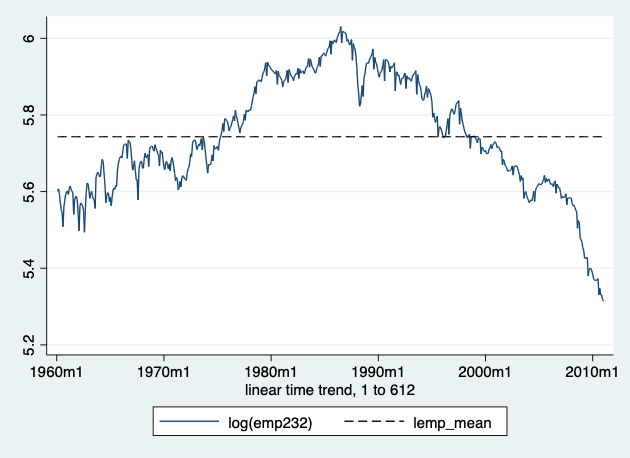
\includegraphics[width=6cm]{photos/lemp.png}
  \caption{Log Employment}
  \label{fig:sub1}
\end{subfigure}%
\begin{subfigure}{.5\textwidth}
  \centering
  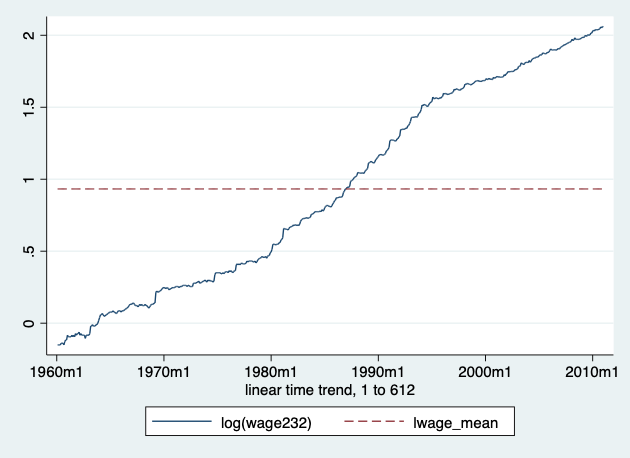
\includegraphics[width=6cm]{photos/lwage.png}
  \caption{Log Wage}
  \label{fig:sub2}
\end{subfigure}
\caption{Two log variables without unit roots}
\label{fig:lemp lwage}
\end{figure}

We can also check for first order autocrrelation by just calculating the correlations. Using this method (that we showed earlier) we get a correlation of 0.992. Even if we were to control for the linear time trend in log wages, we still see a first order sutocorrelation value of 0.995.

By doing the regression with just logged values we get unexpected values. SO we can use growth rates (difference in logarithms) which present no unit root behaviour.

\begin{center}
    {
\def\sym#1{\ifmmode^{#1}\else\(^{#1}\)\fi}
\begin{tabular}{|l*{1}|{c}|}
\toprule
                    &\multicolumn{1}{c}{(1)}\\
                    &\multicolumn{1}{c}{log(emp232)}\\
\midrule
log(minwage)        &       0.364         \\
                    &     (0.030)\sym{***}\\
\addlinespace
log(cpi)            &      -0.616         \\
                    &     (0.028)\sym{***}\\
\addlinespace
linear time trend, 1 to 612&       0.001         \\
                    &     (0.000)\sym{***}\\
\addlinespace
Constant            &       7.747         \\
                    &     (0.080)\sym{***}\\
\midrule
Observations        &         612         \\
\(R^{2}\)           &       0.538         \\
Adjusted \(R^{2}\)  &       0.536         \\
\bottomrule
\multicolumn{2}{l}{\footnotesize Standard errors in parentheses}\\
\multicolumn{2}{l}{\footnotesize \sym{*} \(p<0.10\), \sym{**} \(p<0.05\), \sym{***} \(p<0.01\)}\\
\end{tabular}
}
\end{center}

We are interested in the growth in industry-specific wage and the growth of the overall minimum wage. 
\lstinline{gwage232}$_t = \beta_0 + \beta_1$\lstinline{gmwage}$_t + \beta_2$\lstinline{gcpi}$_t + u_t$, where \lstinline{gcpi} is the approximate monthly rate of inflation.

    {
\def\sym#1{\ifmmode^{#1}\else\(^{#1}\)\fi}
\begin{tabular}{|l*{1}|{c}|}
\toprule
            &\multicolumn{1}{c}{(1)}\\
            &\multicolumn{1}{c}{gwage232}\\
\midrule
gmwage      &       0.151         \\
            &     (0.010)\sym{***}\\
\addlinespace
gcpi        &       0.244         \\
            &     (0.082)\sym{***}\\
\addlinespace
\_cons      &       0.002         \\
            &     (0.000)\sym{***}\\
\midrule
\(N\)       &         611         \\
\(R^{2}\)   &       0.293         \\
adj. \(R^{2}\)&       0.290         \\
\bottomrule
\multicolumn{2}{l}{\footnotesize Standard errors in parentheses}\\
\multicolumn{2}{l}{\footnotesize \sym{*} \(p<0.10\), \sym{**} \(p<0.05\), \sym{***} \(p<0.01\)}\\
\end{tabular}
}
We are able to check if this is an immediate reaction or not:

{
\def\sym#1{\ifmmode^{#1}\else\(^{#1}\)\fi}
\begin{tabular}{|l*{1}|{c}|}
\toprule
            &\multicolumn{1}{c}{(1)}\\
            &\multicolumn{1}{c}{gwage232}\\
\midrule
gmwage      &       0.150         \\
            &     (0.010)\sym{***}\\
\addlinespace
gmwage\_1    &      -0.006         \\
            &     (0.010)         \\
\addlinespace
gmwage\_2    &      -0.001         \\
            &     (0.010)         \\
\addlinespace
gmwage\_3    &      -0.021         \\
            &     (0.010)\sym{**} \\
\addlinespace
gmwage\_4    &      -0.008         \\
            &     (0.010)         \\
\addlinespace
gmwage\_5    &      -0.010         \\
            &     (0.010)         \\
\addlinespace
gmwage\_6    &      -0.001         \\
            &     (0.010)         \\
\addlinespace
gcpi        &       0.291         \\
            &     (0.085)\sym{***}\\
\addlinespace
\_cons      &       0.002         \\
            &     (0.000)\sym{***}\\
\midrule
\(N\)       &         605         \\
\(R^{2}\)   &       0.302         \\
adj. \(R^{2}\)&       0.292         \\
\bottomrule
\multicolumn{2}{l}{\footnotesize Standard errors in parentheses}\\
\multicolumn{2}{l}{\footnotesize \sym{*} \(p<0.10\), \sym{**} \(p<0.05\), \sym{***} \(p<0.01\)}\\
\end{tabular}
}

We can see that the third lag has the highest coefficient and it is significant at the 5\% level.


\section{Serial Correlation in TS Data}

\subsection{Properties of OLS under Serial Correlation}

Our model written in its usual form is:
\[y_t = \beta_0 + \beta_1 x_{t1} + \ldots + \beta_k x_{tk} + u_t\]
Serial correlation implies that the errors $\{u_t: t=1,2,\ldots\}$ are correlated. Luckily our assumptions for unbiasedness and consistency are NOT reliant on no serial correlation. There are some situations where the nature of $x_{tj}$ means that serial correlation in $u_t$ implies that $u_t$ is correlated with $x_{tj}$, but this is rare.

Serially correlated error terms mean that the usual OLS statistical inference is incorrect.

\paragraph{Serial Correlation and goodness of fit}\mbox{} \\

Serial correlation usually does NOT invalidate $R^2, \Bar{R}^2$. It depends on the source of the correlation.

\subsection{Computing Standard Errors Robust to Serial Correlation and Heteroskedasticity}

We treat serial correlation in TS data similarly to how we treated homoskedasticity in CS data. We used to use the optional command: \lstinline{robust}. This would mean the inference will be robust to heteroskedasticity of unknown form. It substitutes constant error variance with heteroskedastic error variance in the formula for standard errors. 

We can compute all inference statistics robust to general forms of serial correlation (approximately). they will be robust to any forms of heteroskedasticity.

For example, we may decide to allow $u_t$ to be correlated with $u_{t-1}, u_{t-2}$ but not errors more than two periods apart. The resulting standard errors are called \textbf{Newey-West Standard Errors}. They are sometimes called \textbf{HAC} (heteroskedasticity and autocorrelation consistent) standard errors.

Just like with heteroskedastic data, applying the \lstinline{newey} command when there is no serial correlation will result in standard errors being too large.

\lstinline{newey y x1 x2 ... xk, lags(q)}, with q=0 this is exactly equivalent to \lstinline{reg y x1 x2 ... xk, robust}.

\subsection{Testing for Serial Correlation}

\begin{shaded}
    In general, we specify:
    \begin{align*}
        H_0:& \text {errors are not serially correlated} \\
        H_1:& \text {errors are serially correlated}
    \end{align*}
    With the AR(1) model,
    \[u_t = \rho u_{t-1} + e_t\]
    where $e_t$ is serially uncorrelated, has zero mean and constant variance. $H_0: \rho = 0$.
\end{shaded}

However, $u_t$ is unobserved. We would have to use residuals and that would depend on an estimated value of $\beta$.

\subsubsection{Testing $\boldsymbol{\rho}$ under Strict Exogeneity}

Provided $x_{tj}$ are strictly exogenous (TS.3) then we can implement the test in three steps.

\begin{mdframed}
    \begin{enumerate}
        \item Estimate the equation:
        
        \[y_t = \beta_0 + \beta x_{t1} + \ldots + \beta_k x_{tk} + u_t, \qquad t=1,2,\ldots,n\]
        
        and save the residuals $\hat{u}_t: t=1,2,\ldots,n$

        \item Run the AR(1) regression: $\hat{u}_t on \hat{u}_{t-1} \forall t$. We do not need to estimate an intercept because the average of $\hat{u}_t$ is almost 0

        \item Compute the usual or heteroskedasticity-robust $t$ statistic for $\hat{\rho}$, and carry out the test $H_0: \rho = 0$.
    \end{enumerate}
\end{mdframed}

    \begin{lstlisting}[caption = Example of Code to do these steps]
        reg y x1 x2 // step 1. regress
        predict uhat, resid // ans save the residual
        g uhat_1 = L.uhat // creating a lag
        reg uhat uhat_1 // step 2. run the AR(1) model

        // step 3. we check the coefficient and p value of this regression to see statistical significance.
    \end{lstlisting}

\subsubsection{Role of Sample Size}

With large $n$ we might reject $\rho = 0$ even if $\hat{\rho}$ is small. With small $n$, we might reject ebem if $\hat{\rho}$ seems quite large.

\subsubsection{Extnesions to the test}

Another test statistic is the Durbin-Watson statistic. Unless the sample size is small, it has little to offer over the simple regression based test. We can add lags to this statistic and use an F test.

\subsubsection{Testing under Contemporaneous Exogeneity}

When strict exogeneity fails, a simple adjustment is needed. All we have to do is add all the explanatory variables along with the lagged residual. We \textbf{must} estimate an intercept because the average is not 0.

So, for the AR(1) test (step 2) we will run, $\hat{u}_)t$ on $\hat{u}_{t-1}, x_{t1}, x_{t2}, \ldots, x_{tk}, t=2,\ldots, n$. We can see that we need to add all the regressors, because $u_{t-1}$ might be correlated with any of the explanatory variables, if the $x_{tj}$ are not strictly exogenous.

One \textbf{must} use this form if one of the explanatory variables, $x_{tj}$ is a lag of $y_t$.

\subsubsection{Why do we test for serial correlation?}

\begin{shaded}
    \begin{enumerate}
        \item \textbf{Lag Choice}: HAC errors require the choice of a lag, and different choices may lead to different standard erros.

        \item \textbf{Efficiency}: Without serial correlation, it is pointless to try to implement estimation methods that improve upon OLS only in the presenceof serial correlation.

        \item \textbf{Misspecification}: We may have specified a model that should not have serial correlation. e.g. an AR(1) model that includes one lag of the dependent variable should not have serial correlation. So we test if we have misspecified.
    \end{enumerate}
\end{shaded}

\subsection{Correcting for Serial Correlation}

If we detect serial correlation, then it must be accounted for. HAC errors as we saw earlier are easy to implement, but these errors may be impractically large.

We can directly model serial correlation and apply \textbf{generalised least squares (GLS)}. For this process though, our regressors \textbf{must be strictly exogenous}.

\subsubsection{GLS with AR(1) Errors}

\begin{shaded}
    Consider the following model with AR(1) errors:
    \begin{gather*}
        y_t = \beta_0 + \beta_1 x_t + u_t \\
        u_t = \rho y_{t-1} + e_t
    \end{gather*}
    For $t\geq 2$, we have
    \begin{equation}
        \label{quasi difference t 2}
        \Tilde{y}_t = (1-\rho) \beta_0 + \beta_1 \Tilde{x}_t + e_t
    \end{equation}
    where 
    \[\Tilde{y}_t = y_t - \rho y_{t-1}, \Tilde{x}_t = x_t - \rho x_{t-1}\]

    For $t=1$, 
    \begin{equation}
        \label{quasi difference t 1}
        \Tilde{y}_1 = \sqrt{1-\rho^2} \beta_0 + \beta_1 \Tilde{x}_1 + \Tilde{u}_1,
    \end{equation}

    where
    \[\Tilde{u}_1 = \sqrt{1-\rho^2} u_1, \Tilde{y}_1 = \sqrt{1-\rho^2}, \Tilde{x}_1 = \sqrt{1-\rho^2}x_1\]

    $\Tilde{x}_t, \Tilde{y}_t$ are called \textit{quasi-differenced} data and they satisfy all Gauss-Markov assumptions.

    \begin{note}
        We are able to add more explanatory variables, we just need to quasi-difference that data as well.
    \end{note}
\end{shaded}

\subsubsection{Are they Feasible Estimators?}

We rarely know the value of $\rho$ and instead must estimate it. Feasible GLS first obtains an estimate for $\rho$ and then uses this to quasi-difference the data.

\begin{mdframed}
    3 steps for FGLS estimation of a model with AR(1) errors:
    \begin{enumerate}
        \item Run the OLS regression of $y_t$ on $x_{t1}, x_{t2}, \ldots, x_{tk}$ and obtain the residual $\hat{u}_t$.

        \item Regress $\hat{u}_t$ on $\hat{u}_{t-1}$ for $t\geq 2$, to obtain an estimate $\hat{\rho}$.

        \item Quasi-differnce the data and run OLS to obtain consistent estimates and asymptotically valid standard errors.
    \end{enumerate}
\end{mdframed}

The easiest way to do this in Stata is to use the \lstinline{prais} command in place of the \lstinline{reg} command.

\subsection{Forecasting}

Forecasting economic time series is very important in some branches of economics. With forecasting we make informed guesses about the future $(t+h)$ given what we know today $(t)$.

\subsubsection{Stationary Univariate Model}

For regression based forecasting, let us begin with a univariate model:
\begin{mdframed}
    \begin{gather*}
        y_t = \delta_0 + \alpha_1 y_{t-1} + \gamma_1 z_{t-1} + \epsilon_t\\
        E(\epsilon_t|I_{t-1}) = 0, Var(\epsilon_t|I_{t-1})=\sigma^2
    \end{gather*}
    where $I_{t-1}$ contains $y$ and $z$ dated at time $t-1$ and earlier. 
\end{mdframed}

Now, the forecast of $y_{t+1}$ at time $t$ is $\delta_0 + \alpha_1 y_t + \gamma_1 z_t$. If we have estimated the parameters, we can plug in the values of $y_t$ and $z_t$ to yield a forecasted result.

The forecast error associated with this 1-step-ahead forecast is:
\[\hat{\epsilon}_{t+1} = y_{t+1} - \hat{y}_{t+1}\]
giving us the forecast interval of:
\[\hat{y}_{t+1} \pm 1.96 \cdot se(\hat{\epsilon}_{t+1}\]

\begin{mdframed}
    \begin{equation}
        \label{se epsilon forecast}
        se(\hat{\epsilon}_{t+1} = \left\{ [se(\hat{y}_{t+1})]^2 + \hat{\sigma}^2\right\}^{\frac{1}{2}}
    \end{equation}

    We know that there are two sources of uncertainty: uncertainty from the forecast ($se(\hat{y}_{t+1})$) and the uncertainty from the regression ($\hat{\sigma}$), given as the standard error of the regression.

    To find $se(\hat{y}_{t+1})$, we regress $y_t$ on $(y_t - y_n)$ and $(z_t - z_n)$ and use the standard error of the intercept.
\end{mdframed}

\subsubsection{Forecast Performance}

To asses the forecast performance m-steps ahead, we use either root mean squared error (RMSE):
\begin{mdframed}
    \begin{equation}
        \label{forecast rmse}
        RMSE = \left[ \dfrac{1}{m}\sum_{h=0}^{m-1} \hat{\epsilon}^2_{t+h+1}\right]^{1/2}
    \end{equation}
\end{mdframed}

or we can use Mean Absolute Error (MAE):
\begin{mdframed}
    \begin{equation}
        \label{mean absolute error mae}
        MAE = \dfrac{1}{m}\sum_{h=0}^{m-1}|\hat{\epsilon}_{t+h+1}|
    \end{equation}
\end{mdframed}
In both cases, we prefer small values.

\section{Advanced Time Series Topics}

\subsection{Stationarity and Non-stationarity}

\begin{figure}[h]
    \centering
    \subfloat[\centering Deterministic Trend]{{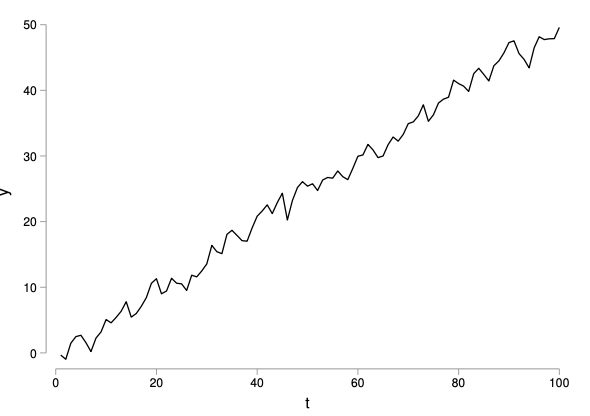
\includegraphics[width=7cm]{photos/deterministic trend.png} }}%
    \qquad
    \subfloat[\centering Stochastic Trend]{{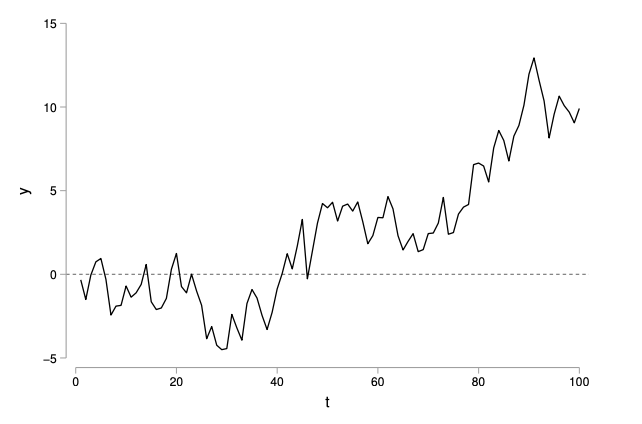
\includegraphics[width=7cm]{photos/unit root.png} }}%
    \caption{Time Trends}%
    \label{fig:trends}%
\end{figure}

A time series can possess a deterministic or stochastic trend. A time series with a \textbf{unit root} is said to have a stochastic trend. It is possible to have both. If a time series has either or both trends, it is said to be non-stationary.

\paragraph{Trend Stationary Processes} are ones that have only a deterministic trend. These kinds fo processes are very easily handled.

\paragraph{Difference stationary or Unit root processes} are time series with stochastic trends.

\paragraph{Order of Integration} is the number of unit roots possessed by a time series.

\begin{figure}[h]
    \centering
    \subfloat[\centering I(0) Process]{{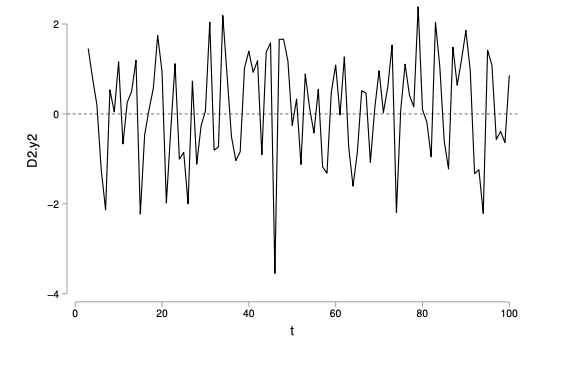
\includegraphics[width=7cm]{photos/i0.png} }}%
    \qquad
    \subfloat[\centering I(2) Process]{{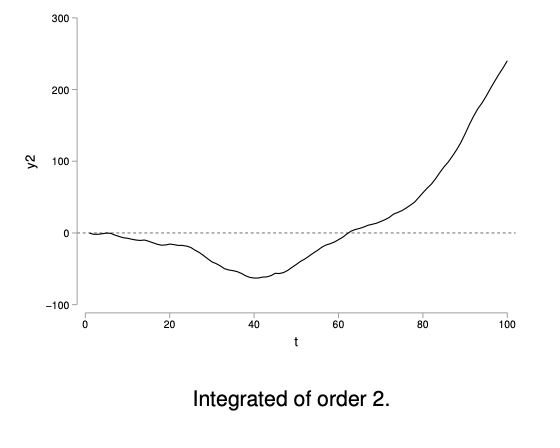
\includegraphics[width=7cm]{photos/i2.png} }}%
    \caption{Ordered of Integration}%
    \label{fig:i0 i2}%
\end{figure}

Our I(0) process in Figure \ref{fig:i0 i2} has no unit root and is said to be integrated of order zero.

We need to make sure we know if our time series is a unit root process. Many economic and financial series appear to have at least one unit root. I(0) and unit root processes have different statistical; properties and consequently behave differently.

Example: hypothesis tests that are valid on I(0) processes may be invalid and very misleading when applied to unit roots. The statistic properties of commonly used estimators may change when they are used to estimate regression equations that contain unit root processes.

\textbf{Asymptotic theory} is invalid when applied to unit root processes. What we are most concerned about is whether our time series is I(0) or not.

\begin{mdframed}
    \paragraph{Independently and Identically Distributed} \mbox{}

    A time series $\{y_t\}$, is i.i.d which is denoted:
    \[y_t \sim i.i.d(0,\sigma^2),\]
    if
    \begin{align*}
        E(y_t) &= 0 \forall t, \\
        Var(y_t) &= \sigma^2 \forall t
    \end{align*}
    and $y_t$ and $y_{t-j}$ are \textbf{independent random variables} $\forall j \neq0$
\end{mdframed}


\begin{mdframed}
    \paragraph{White Noise} \mbox{}

    A time series, $\{y_t\}$, is \textbf{white noise}, which is denoted by
    \[y_t \sim WN(0,\sigma^2),\]
    if
    \begin{align*}
        E(y_t) &= 0 \forall t, \\
        Var(y_t) &= \sigma^2 \forall t \\
        Cov(y_t, y_{t-j}) &= 0 \forall j \neq 0. 
    \end{align*}
\end{mdframed}

A time series is white noise if it has a zero mean, a constant variance and is serially uncorrelated.

\subsection{Covariance Stationary}
\begin{mdframed}
    \paragraph{Covariance Stationary} \mbox{}

    The time series 
    \[\{y_t: t - \ldots -2, -1, 0, 1, 2, \ldots \}\]
    is \textbf{covariance stationary} if
    \begin{enumerate}
        \item $E(y_t) = \mu <\infty, \forall t$
        \item $Var(y_t) = E[(y_t-\mu)^2] = \gamma_0 < \infty, \forall t$
        \item $Cov(y_t, y_{t-j}) = E[(y_t-\mu)(y_{t-j}-\mu)] = \gamma_j <\infty, \forall t,j$
    \end{enumerate}
    That is, the mean is finite and time-invariant, the variance is finite and time-invariant and the covariance between any pair in the time series depends only on the time interval separating them and not on time itself.
\end{mdframed}

\subsubsection{Is AR(1) covariance stationary}

Consider
\[y_t = \varphi y_{t-1} + e_t\]

This equation implies 
\begin{equation}
\begin{aligned}
 y_{t-1}&=\varphi y_{t-2}+e_{t-1} \\
 y_{t-2}&=\varphi y_{t-3}+e_{t-2} \\
&\vdots
\end{aligned}
\end{equation}

Assume that er have an initial value of $y, y_0$ and that $e_t \sim WN(0,\sigma^2)$.

Recursive substitution gives us:
\begin{equation}
\begin{aligned}
& E\left(y_t\right)=\varphi^t y_0 \\
& \operatorname{Var}\left(y_t\right)=\left[1+\varphi^2+\left(\varphi^2\right)^2+\ldots \ldots+\left(\varphi^2\right)^{t-1}\right] \sigma^2 \\
& \operatorname{Cov}\left(y_t, y_{t+j}\right)=\varphi^j \sigma^2\left[1+\varphi^2+\left(\varphi^2\right)^2+\ldots . .+\left(\varphi^2\right)^{t-1+j}\right]
\end{aligned}
\end{equation}

You can see that each of these terms contains $t$ meaning that they are time-variant and therefore not covariance stationary. Luckily we have the following lemma:

\begin{lemma}
If 
\[|\varphi|<1\]
then
\begin{equation}
\operatorname{Lim}_{t \rightarrow \infty}\left[1+\varphi^2+\left(\varphi^2\right)^2+\ldots \ldots+\left(\varphi^2\right)^t\right]=\frac{1}{1-\varphi^2}
\end{equation}
\end{lemma}

Using the lemma it can be shown that:

\begin{equation}
\begin{aligned}
& \operatorname{Lim}_{t \rightarrow \infty} E\left(y_t\right)=\operatorname{Lim}_{t \rightarrow \infty}\left(\varphi^t\right) y_0=y_{t \rightarrow \infty}\left[\operatorname{Lim}\left(\varphi^t\right)\right]=0 . \\
& \operatorname{Lim}_{t \rightarrow \infty} \operatorname{var}\left(y_t\right)=\frac{\sigma^2}{\left(1-\varphi^2\right)} \\
& \operatorname{Lim}_{t \rightarrow \infty} \operatorname{Cov}\left(y_t, y_{t+j}\right)=\frac{\sigma^2 \varphi^j}{\left(1-\varphi^2\right)}
\end{aligned}
\end{equation}

All the mean, variance and covariance are all now time-invariant and the covariance is only a function of $j$ and not $t$. Therefore if we have the AR(1) process:

\[y_t = \varphi y_{t-1} + e_t, |\varphi|<1\]

then the mean, variance and the $j$th autocovariance of $y_t$ are independent of time as $t\rightarrow\infty$, we say that is, $y_t$ is \textbf{asymptotically stationary}.

\begin{mdframed}
    \subsubsection*{Asymptotic Stationarity}

    \begin{theorem}
        If
        \[y_t = \varphi y_{t-1} + e_t\]
        where
        \[e_t \sim WN(0,\sigma^2),\]
        then $y_t$ is \textbf{asymptotically stationary} if
        \[|\varphi| <1\]
    \end{theorem}
\end{mdframed}


\begin{figure}[h]
    \centering
    \subfloat[\centering AR(1) with $\varphi = 0.8$]{{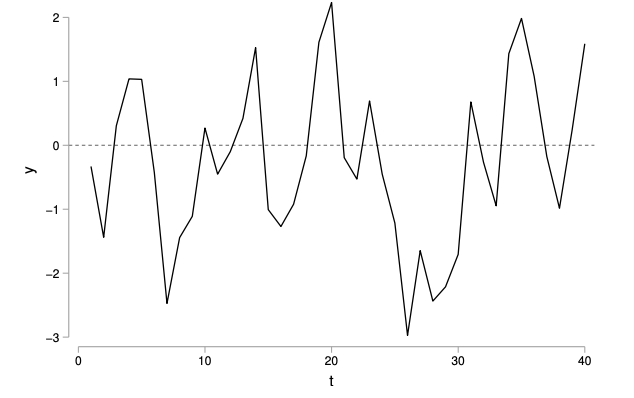
\includegraphics[width=7cm]{photos/varphi 0.8.png} }}%
    \qquad
    \subfloat[\centering AR(1) with $\varphi = 1.1$]{{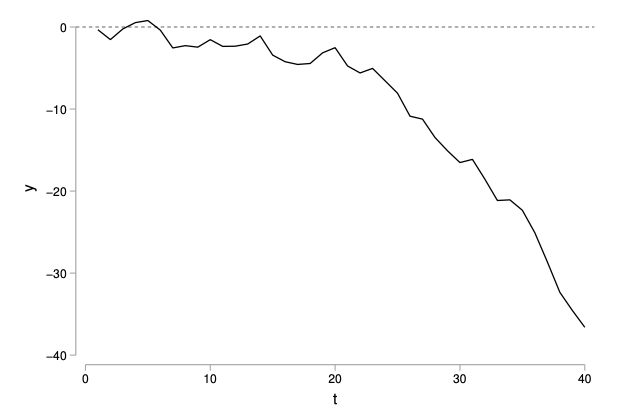
\includegraphics[width=7cm]{photos/varphi 1.1.png} }}%
    \caption{Two AR(1) processes with different values for $\varphi$}%
    \label{fig:asymptotic stationarity}%
\end{figure}

\subsection{Trend Stationary and Difference Stationary Processes}

\subsubsection{Deterministic Trend Example}

A time series that varies systematically with time in a deterministic fashion is said to possess a \textbf{deterministic trend}. For example:
\[y_t = 0.9 + 0.2t + 0.6y_{t-1} + e_t\]
varies in a deterministic way with time due to the presence of the deterministic term $0.2t$.

\subsubsection{Stochastic Trend Example}

A time series which has a unit root is said to possess a \textbf{stochastic trend}. For example:
\[y_t = y_{t-1} + e_t,\]
has a stochastic trend because $\varphi = 1$.

\subsubsection{Both Trends}

A series can have both deterministic and stochastic trends. For example:
\[y_t = 0.2t + y_{t-1} + e_t\]
has \textbf{both} a deterministic trend and a stochastic trend

\begin{figure}[h]
    \centering
    \subfloat[\centering Deterministic Trend]{{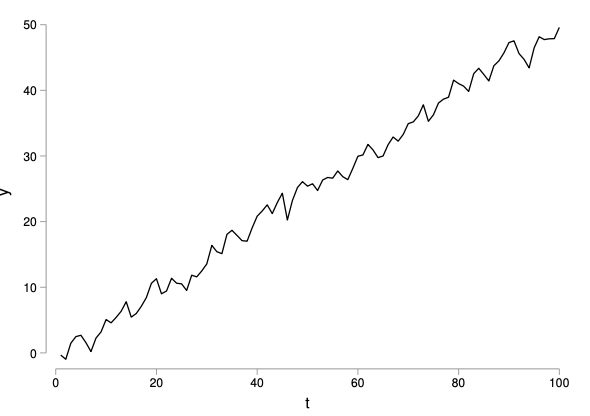
\includegraphics[width=7cm]{photos/deterministic trend.png} }}%
    \qquad
    \subfloat[\centering Stochastic Trend (Unit Root Process)]{{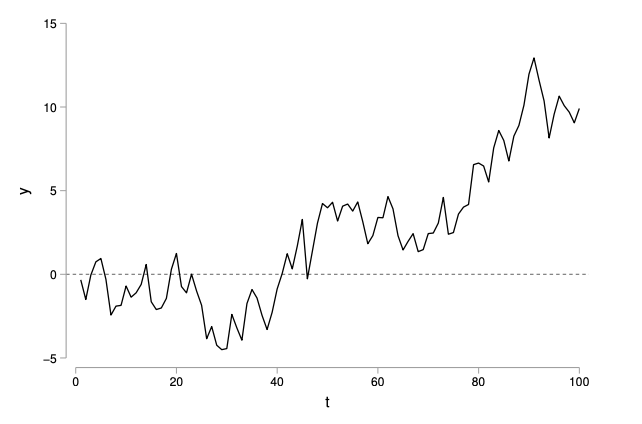
\includegraphics[width=7cm]{photos/unit root.png} }}%
    \qquad
    \subfloat[\centering Both Trends]{{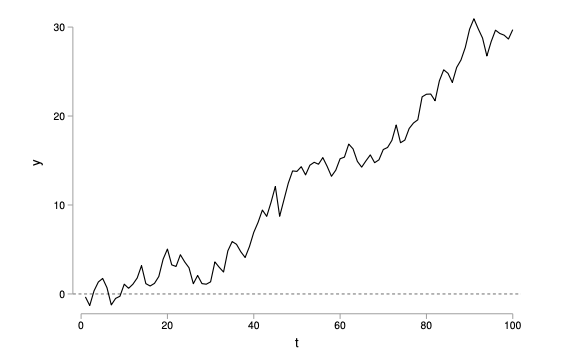
\includegraphics[width=7cm]{photos/both trends.png} }}%
    \caption{The different trends a time series can have}%
    \label{fig:trends2}%
\end{figure}

\subsubsection{Implications}

If a time series possesses a deterministic and/or a stochastic trend, the mean and/or the variance of the time series will be time-dependent and the series will be non-stationary. The trend stationary processes can be easily handled.

\begin{mdframed}
\subsubsection{Trend Stationary Example}
let
\[y_t = a + bt + z_t\]
where $a+bt$ is a deterministic component and $z_t$ is the stochastic or random component.

Assume that $z_t$ is an AR(1) process given by:
\[z_t = \varphi z_{t-1} - e_t\]
where $e_t \sim i.i.d(0, \sigma^2)$.

We can show that $y_t$ is a trend stationary process when $|\varphi|<1$.

Rearranging gives:
\[z_t = y_t - a - bt\]
then we have:
\[\varphi z_{t-1} = \varphi (y_{t-1} - a - b(t-1))\]

if we define $y^*_t = (y_t-a-bt)$ and $y_{t-1}^* = \varphi(y_{t-1}-a-b(t-1))$ we have:
\[y_t^* = \varphi y_{t-1}^* + e_t\]
since $e_t = z_t - \varphi z_{t-1}$.
\end{mdframed}

Because we have been able to convert the original time series $y_t$ into an asymptotically stationary series by simply removing the deterministic trend, $a+bt$, $y_t$ is called a \textbf{trend stationary process (TSP)}.

However $y_t$ is still not stationary, but it is I(0). $y^*_t$ is asymptotically stationary and I(0).


\begin{mdframed}
\subsubsection{Difference Stationary Example}

let
\[y_t = a +bt + z_t\]
where 
\[z_t = z_{t-1} + e_t\]
and $e_t \sim i.i.d(0,\sigma^2)$

\textbf{$z_t$ is now assumed to be a unit root process}. From our first equation we have:
\[y_{t-1} = a+b(t-1) + z_{t-1}\]
Subtracting the second equation from the first we get:
\[y_t = b_t + y_{t-1} + e_t\]
since $e_t = z_t - z_{t-1}$
\end{mdframed}
Because $y_t$ must be differenced once to male it stationary, we call it a \textbf{difference stationary process (DSP)}.


\begin{figure}[h]
    \centering
    \subfloat[\centering I(1) process before differencing]{{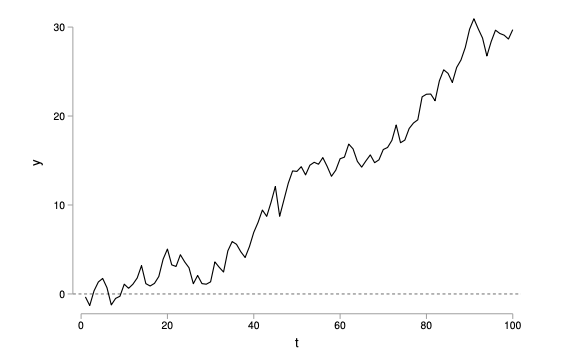
\includegraphics[width=7cm]{photos/both trends.png} }}%
    \qquad
    \subfloat[\centering I(1) process after differencing]{{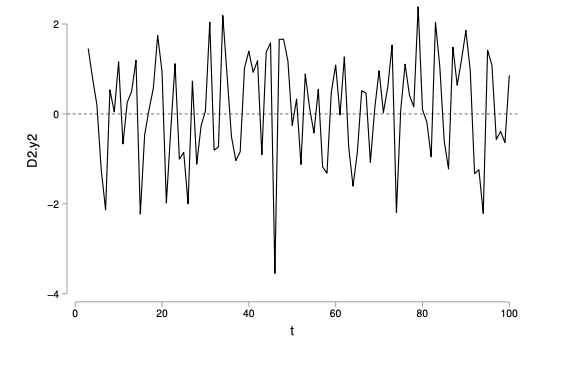
\includegraphics[width=7cm]{photos/i0.png} }}%
    \caption{I(0) pre- and post-differencing}%
    \label{fig:differencing I(1)}%
\end{figure}

\subsubsection{Random Walk with drift}

The process 
\[y_t = b + y_{t-1} + e_t\]

is known as a random walk with drift. The name comes from the fact that
\[E(y_t - y_{t-1}) = b\]
on average the time series changes or "drifts" by the amount $b$ between one time period and the next. When a random walk contains a drift, there is a deterministic and stochastic trend.

In both random walk and random walk with drift, through recursive substitution we have:
\[\text{ Random Walk: } y_t = y_0 + s_t\]
\[\text{ Random Walk with Drift: } y_t =bt + y_0 + s_t\]

In both instances $s_t=\sum_{u=1}^t e_i$. $s_t$ is itself a random walk since $s_t = s_{t-1} + e_t$. The presence of $s_t$ tells us that $y_t$ has a stochastic trend.

\subsubsection{TSP vs. DSP}

Consider
\[y_t = a + bt + \varphi y_{t-1} + e_t\]
where $a$ and $b$ could be 0.
\begin{itemize}
    \item When $|\varphi|<1$ we have a \textbf{trend stationary process}. We can conduct statistical inference using conventional methods like t and F tests.
    \item When $|\varphi|=1$ we have a difference stationary process. The estimated coefficients are a nonstandard distribution, meaning we cannot rely on conventional econometric methods.
\end{itemize}

\textbf{TSP has a short/finite memory}. Take
\[y_t = a + bt + z_t\]
if we update this to period $t+j$ we get:
\[y_{t+j} = a + b(t+j) + z_{t+j}.\]

Through recursive substitution of $z_{t+j}$ we get:
\begin{equation}
z_{t+j}=e_{t+j}+\varphi e_{t+j-1}+\varphi^2 e_{t+j-2}+\cdots+\varphi^j e_t+\ldots
\end{equation}

This implies:
\begin{equation}
\frac{\partial y_{t+j}}{\partial e_t}=\varphi^j
\end{equation}

Because $|\varphi|<1$ the effect of the shock $e_t$ goes to 0 as $j\rightarrow\infty$.

\textbf{A DSP has long/infinite memory}. Take
\[y_t = bt + y_0 + e_t + e_{t-1} + \ldots + e_1\]
and we update this to period $t+j$ we get:

\[y_{t+j} = b(t+j) + y_0 + e_{t+j} + e_{t+j-1} + \ldots + e_t + e_{t-1} + \ldots + e_1\]

This implies that:
\begin{equation}
\frac{\partial y_{t+j}}{\partial e_t}=1 \forall j \geq 0
\end{equation}
The effect of a random shock to the time series in period $t$ never declines and never dies out.

\clearpage
\subsection{Dickey-Fuller test}

\begin{mdframed}
    \paragraph{Unit Root} \mbox{}

    In the case of the following AR(1) processes:
    \begin{align*}
        y_t &= \varphi y_{t-1} + e_t \\
        y_t &= a + \varphi y_{t-1} + e_t \\
        y_t &= a + bt + \varphi y_{t-1} + e_t \\
        e &\sim WN(0,\sigma^2)
    \end{align*}
    $y_t$ is said to have a \textbf{unit root} iff.
    \[|\varphi|=1\]
\end{mdframed}

Because these AR(1) processes have a unit root the order of integration is 1. Differencing an I(1) series once renders it stationary.

\begin{figure}[h]
    \centering
    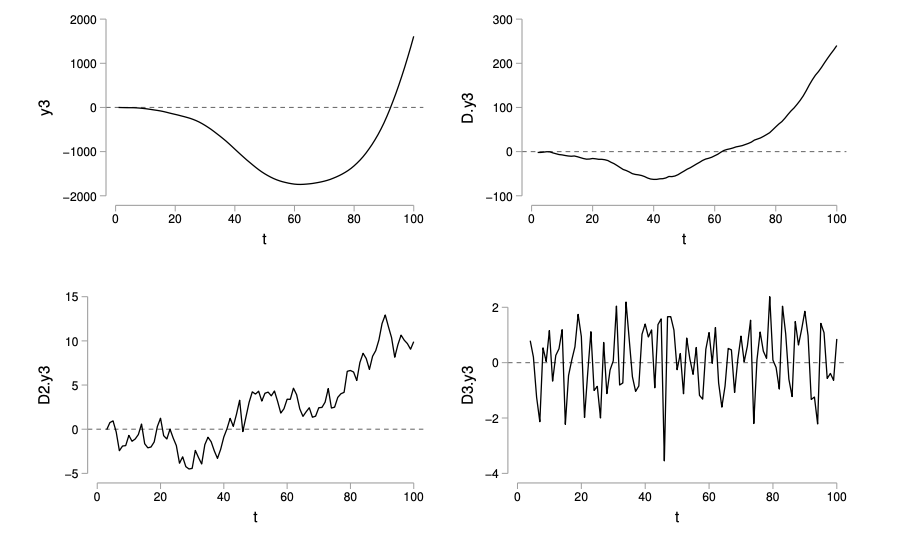
\includegraphics[width=15cm]{photos/i3.png}
    \caption{I(3) process at the different levels of differencing}
    \label{fig:i3 being differenced}
\end{figure}

\subsubsection{Formulating DF test}

In economic and financial time series we tend to have \textbf{positive} autocorrelation ($\varphi=1$) at lag 1. So that is what we test for rather than $\varphi=-1$. It is most convenient to test for a coefficient = 0, therefore we create a new coefficient:
\[\gamma = \varphi - 1\]
From our equations in the unit root definition, we can subtract $y_{t-1}$ from both sides giving us:
\begin{align*}
    y_t - y_{t-1} &= (\varphi-1)y_{t-1} + e_t \\
    dy_t &= \gamma y_{t-1} + e_t \\
    \\
    y_t - y_{t-1} &= a + (\varphi - 1) y_{t-1} + e_t \\
    dy_t &= a + \gamma y_{t-1} + e_t \\
    \\
    y_t - y_{t-1} &= a + bt + (\varphi-1)y_{t-1} + e_t \\
    dy_t &= a + bt + \gamma y_{t-1} + e_t
\end{align*}

Because $\varphi = 1$ iff. $\gamma =0$, to test the null that $y_t$ has a unit root in any of the specified equations, we can test the null that $\gamma=0$.

\begin{shaded}
\subsubsection{The test}

We test :
\begin{align*}
H_0&: \gamma=0 \\
H_1&: \gamma<0
\end{align*}
We compare:
\[t = \dfrac{\hat{\gamma}}{se(\hat{\gamma})}\]
to an appropriately chosen critical value, $t_{crit}$. We reject the null that $y_t$ has a unit root if
\[t_{calc}>t_{crit}\]


\end{shaded}

Dickey and Fuller found that the t-stat has a non-\textbf{standard asymptotic distribution} under the null, so we must use different critical values.

These critical values are larger, and because of this, we may incorrectly reject the null of the unit root if we were to use the values from the standard normal distribution.

\subsection{Augmented Dickey-Fuller Test}

We could have a case were we have AR(1) errors, that is,
\[y = \varphi y_{t-1} + u_t\]
where 
\[u_t = \theta_1 u_{t-1} + e_t, |\theta_1|<1,\]
and $e_t \sim i.i.d(0,\sigma^2)$.

Using
\[y_t=\varphi_1 y_{t-1}+\theta_1 u_{t-1}+e_t\]
and that
\[u_{t-1}=y_{t-1}-\varphi_1 y_{t-2},\]
we have
\begin{align*}
    y_t&=\left(\varphi_1+\theta_1\right) y_{t-1}-\varphi_1 \theta_1 y_{t-2}+e_t \\
&=b_1 y_{t-1}+b_2 y_{t-2}+e_t \\
\end{align*}
where
\[b_1 \equiv\left(\varphi_1+\theta_1\right), b_2 \equiv-\varphi_1 \theta_1, e_t \sim i . i . d\left(0, \sigma^2\right).\]

So we have rewritten our AR(1) process with stationary AR(1) errors as an AR(2) model:
\[y_t =b_1 y_{t-1}+b_2 y_{t-2}+e_t\]

This shows us that by adding an additional lag of the dependent variable as a regressor we have been able to remove the autocorrelation of order 1 in the error term of our regression. 
 
The \textbf{Augmented Dickey-Fuller} test tests for a unit root in $y_t$ when the error term in the model follows an AR(p) process.

\begin{mdframed}
\paragraph{Implementing the test} \mbox{}

If we take Model 1 from the Unit Root definition:
\[y_t = \varphi y_{t-1} + u_t\]
and now say $u_t = \theta_1 u_{t-1} + e_t, |\theta_1|<1$ and $e_t\sim i.i.d(0,]sigm
^2)$. Then from the same work earlier in the section, we get the equation:

\[y_t = b_1 y_{t-1} + b_2 y_{t-2} + e_t\]

we can do the following:
add and subtract $b_2 y_{t-1}$ on the RHS:
\begin{align*}
    y_t &= b_1 y_{t-1} \boldsymbol{+ b_2 y_{t-1}}+ b_2 y_{t-2} \boldsymbol{- b_2 y_{t-1}} + e_t \\
    &= (b_1 + b_2) y_{t-1} - b_2 dy_{t-1} + e_t
\end{align*}
subtracting $y_{t-1}$ from both sides:
\begin{align*}
    y_t - \boldsymbol{y_{t-1}} &= (b_1 + b_2 - \boldsymbol{1})y_{t-1} - b_2 dy_{t-1} + e_t \\
    dy_t &= \gamma y_{t-1} + \alpha_1 dy_{t-1} + e_t
\end{align*}
where $ \gamma \equiv (b_1+b_2-1), \alpha_1 \equiv -b_2$.

We test:
\begin{align*}
    H_0&: \gamma = 0 \\
    H_1&: \gamma < 0
\end{align*}
and we have the t-statistic
\[t = \dfrac{\hat{\gamma}}{se(\hat{\gamma})}\]

This can be done with any of the models we have looked at.
\end{mdframed}

\subsubsection{Generalising the results}

We can look at the case where $y_t$ is an AR(p) process given by one of the following:

\begin{equation}
\begin{aligned}
& y_t=b_1 y_{t-1}+b_2 y_{t-2}+\ldots .+b_p y_{t-p}+e_t \\
& y_t=a+b_1 y_{t-1}+b_2 y_{t-2}+\ldots .+b_p y_{t-p}+e_t \\
& y_t=a+b t+b_1 y_{t-1}+b_2 y_{t-2}+\ldots .+b_p y_{t-p}+e_t
\end{aligned}
\end{equation}

By using the same techniques from earlier we have:

\begin{equation}
\begin{aligned}
& d y_t=\gamma y_{t-1}+\alpha_1 d y_{t-1}+\ldots . .+\alpha_{p-1} d y_{t-(p-1)}+e_t \\
& d y_t=a+\gamma y_{t-1}+\alpha_1 d y_{t-1}+\ldots .+\alpha_{p-1} d y_{t-(p-1)}+e_t, \\
& d y_t=a+b t+\gamma y_{t-1}+\alpha_1 d y_{t-1}+\ldots . .+\alpha_{p-1} d y_{t-(p-1)}+e_t
\end{aligned}
\end{equation}

where $\gamma \equiv (b_1 + b_2 + \ldots + b_p -1)$. We always do the same test and have the same t-statistic formula. \textbf{There are different critical values for each of the different models.}


\subsubsection{Complications}

The critical values that we use are based on the assumption that the underlying process:
\[dy_t = \gamma y_{t-1} + e_t\]
where $e_t \sim i.i.d(0,\sigma^2)$. \textbf{However}, in general, the asymptotic null distribution of 
\[t=\dfrac{\hat{\gamma}}{se(\hat{\gamma})}\]
depends on \textbf{both} the form of the underlying process and the form of the estimated regression equation. There are instances when $t \overset{a}{\sim} SN$. We might conclude that there is a unit root when the series is I(0).


\section{Pooled Cross Sections and Panel Data}


\subsection{Cointegration}

Once we have established $y_t$ and $x_t$ are two I(1) processes, how do we analyse them without encountering the spurious relationship problem?

If there exists one or more linear combinations of $y_t$ and $x_t$ that are I(0) then we say that $y_t$ and $x_t$ are \textbf{cointegrated}. If such a linear relationship exists, they constitute long-run equilibrium relationships between the variables.

If we have $y_t$ and $x_t$ are two cointegrated processes then 
\[y_t - \beta x_t\]
is an I(0) process, meaning it has a constant mean, variance and autocorrelation depend only on the time distance between any two variables in the series, and it is asymptotically uncorrelated. $\beta$ is called the cointegration parameter. For \textit{uniqueness} we fix $y_t$ at unity.

If we do not know the value of $\beta$ we can run the regression:
\[y_t = \alpha + \beta x_t + u_t\]
and get $\hat{u_t}= y_t - \hat{\alpha} -\hat{\beta}x_t$.

When we test for a unit root in $\hat{u_t}$, we update the DF critical values to account for the estimation of $\beta$. This is known as the \textbf{Engle-Granger test}.

\begin{equation}
\begin{aligned}
&\text { Asymptotic critical values for cointegration test: no time trend }\\
&\begin{array}{lllll}
\hline \text { Specification } & 1 \% & 2.5 \% & 5 \% & 10 \% \\
\hline d \hat{u}_t=a+\gamma \hat{u}_{t-1}+e_t & -3.90 & -3.59 & -3.34 & -3.04 \\
\hline
\end{array}
\end{aligned}
\end{equation}
We can add lags of $d\hat{u}_t$ if $d\hat{u}_t$ is serially correlated, and use the \textbf{same} critical values here.

\paragraph{Extension: Random walk with drift} \mbox{}

Cointegration requires that $y_t - \beta x_t$ be an I(0) process \textbf{and trend free}. When $\{y_t\}$ and $\{x_t\}$ contains drift terms, $y_t - \beta x_t$ will generally be a trend-stationary process. We can test for cointegration by running the regression
\[y_t = \alpha + \eta t + \beta x_t + u_t\]
and collecting $\hat{u}_t = y_t - \hat{\alpha} - \hat{\eta} t - \hat{\beta} x_t $. The critical values we use now have to take into account the estimation of $\beta$ and $\eta$.

\begin{equation}
\begin{aligned}
&\text { Asymptotic critical values for cointegration test: linear time trend }\\
&\begin{array}{lllll}
\hline \text { Specification } & 1 \% & 2.5 \% & 5 \% & 10 \% \\
\hline d \hat{u}_t=a+\gamma \hat{u}_{t-1}+e_t & -4.32 & -4.03 & -3.78 & -3.50 \\
\hline
\end{array}
\end{aligned}
\end{equation}

again, we can add lags if $d\hat{u}_t$ is serially correlated and use the same critical values reported here.

\paragraph{Inference on $\beta$} \mbox{}

When $\{y_t\}$ and $\{x_t\}$ are cointegrated in
\[y_t = \alpha + \beta x_t + u_t\]
the t-statistic for $\hat{\beta}$ does not necessarily have an approximate t distribution. Given $\{x_t\}$ is I(1), strict exogeneity requires that $\{u_t\}$ is uncorrelated with $\{dx_s\} \forall t,s$. We are not comparing $u_t$ to $x_t$ because $x_t$ is I(1) while $u_t$ is I(0). There is no point in comparing the two.

The solution to this is we add lags and leads of $\{dx_s\}$ to the cointegrating equation to remove the past, present and future correlation. This is what we call the \textbf{expanded model}.

\begin{equation}
\begin{aligned}
y_t= & \alpha_0+\beta x_t+\phi_0 d x_t+\phi_1 d_{t-1}+\phi_2 d x_{t-2} \\
& +\gamma_1 d x_{t+1}+\gamma_2 d x_{t+2}+e_t
\end{aligned}
\end{equation}

If $r_t$ is serially correlated we can use heteroskedasticity autocorrelation (HAC) robust standard errors.

 Our new error term $e_t$ is uncorrelated with each $dx_s$ \textbf{in the equation}. Because $dx_s$ is I(0), the correlation between further lags/leads if $dx_S$ with the specified lags/leads will approach 0. This implies that the correlation of further lags/leads of $dx_s$ and $e_t$ will approach 0.

 The $\beta$ we estimate here is called the \textbf{leads and lags estimator} of $\beta$. IF we have a regression output we will want to test the $\beta$ coefficient against the value of \textbf{1}.

 \paragraph{What if x and y are not cointegrating} \mbox{}

 To model their relationship we first difference the series to obtain $dy_t$ and $dx_t$ and regress these I(0) series on one another,
 \[dy_t = \alpha_0 + \gamma_0 dx_t + u_t\]
 we can add whatever lag dynamics we would like to the model e.g. $dy_{t-1}, dx_{t-1}$.

 \hl{We cannot interpret the coefficient on the levels, only on the differences}.

 \subsubsection{Error Correction Model}

 When $\{y_t\}$ and $\{x_t\}$ are cointegrated, we learn about their long-run relationship from the cointegration (levels) equation. We can expand the differenced equation to evaluate their short-run relationship:
 \begin{equation}
d y_t=\alpha_0+\gamma_0 d x_t+\delta\left(y_{t-1}-\beta x_{t-1}\right)+u_t
\end{equation}

We can add the $y_{t-1}-\beta x_{t-1}$ component because it is I(0). This component can also be seen as the error in the previous period. This model in the current period adjusts for this deviation using $\delta<0$.

When $y_{t-1}<\beta x_{t-1}$, there was a negative deviation from the mean in the previous period, and $\delta(y_{t-1}-\beta x_{t-1})$ corrects it by pushing it back to the equilibrium.

This allows us to study the short-run dynamics in the relationship between $y$ and $x$.

\subsection{Pooled Cross Section and Difference in Differences}

Data obtained by pooling cross-sections are very useful. We can use a pooled cross-section (PCS) whenever a survey is repeated over time with new random samples obtained each period. This means that the survey does \textbf{not} track the same individuals.

PCSs are at the foundation of difference-in-differences (DID) estimation. We want data before and after the intervention (treatment) and there to be one control group (at least) and one "treatment" group.

Often the treatment is of a yes/no format but other non-binary treatments such as class size can be handled too.

Outcomes are observed for the two groups over two time periods. The treatment group is exposed to the "treatment" in the second period but not the first. The control group is not exposed to the treatment during either.

\subsubsection{DID model}

Let $d2$ be a time period indicator equal to 1 for a unit in the second period.

\begin{equation}
    y = \beta_0 + \beta_1 dB + \delta_0 d2 + \delta_1 d2 \times dB + u
\end{equation}

where $dB$ is the change in the treatment group.

\begin{table}[h]
    \centering
    \begin{tabular}{|l|l|l|l|}
\hline & Before (1) & After (2) & After - Before \\
\hline Control $(\mathrm{A})$ & $\beta_0$ & $\beta_0+\delta_0$ & $\delta_0$ \\
\hline Treatment $(\mathrm{B})$ & $\beta_0+\beta_1$ & $\beta_0+\delta_0+\beta_1+\delta_1$ & $\delta_0+\delta_1$ \\
\hline Treatment - Control & $\beta_1$ & $\beta_1+\delta_1$ & $\delta_1$ \\
\hline
\end{tabular}
    \caption{Effects on Treatment Group vs Control Group}
    \label{tab:diff in diff}
\end{table}

In "after" $d2=1$. For "Treatment (B)" $dB=1$.

$dB$ captures possible differences between the treatment and control groups prior to the policy change. This difference is shown in $\beta_1$.

$d2$ captures aggregate factors that would cause changes in $y$ over time even in the absence of an intervention. $\delta_0$ is the change in the mean of the control group.

The coefficient of interest is $\delta_1$, the difference in the average changes over time for the treatment and control groups. Often called the \textbf{average treatment effect}. If $y$ is a logarithm then $\delta_1$ is a proportionate effect.

\hl{We could just do this all using the averages from each period, but using OLS we can use heteroskedasticity-robust errors, which allows different group/time period variances in the regression framework}.

\begin{shaded}
\paragraph{Intuition} \mbox{}

The difference in averages over time of the treatment group, $\Bar{y}_{B,2} - \Bar{y}_{B,1}$, attributes all change to the intervention.

The difference in treatment and control averages post-treatment, $\Bar{y}_{B,2} - \Bar{y}_{A,2}$, attributes any differences in the groups to the treatment.

\[\hat{\delta}_1=\left(\bar{y}_{B, 2}-\bar{y}_{B, 1}\right)-\left(\bar{y}_{A, 2}-\bar{y}_{A, 1}\right)\]

This shows that we are comparing the change in means for the treatment to the change in mean for the control.
    
\end{shaded}

\begin{mdframed}
    \textbf{Example: Worker's Compensation}

    We study the relationship between the length of injury leave and changes to injury compensation. Suppose a policy increased the cap on weekly earnings that were covered by worker's compensation.

    Low earners would not be affected by this policy as they continue to receive the same compensation after the intervention. 

    High earners would have more incentive to stay on worker's compensation for longer because it had become less costly to be on injury leave (because they are getting more compensation).

    If we run a DID: \lstinline{reg ldurat afchnge highearn afhigh}, where \lstinline{ldurat} is the log of duration of benefits in weeks, \lstinline{afchnge} indicates the period after the intervention, \lstinline{highearn} is an indicator for the treatment group of high earners affected by the intervention, and \lstinline{afhigh} is the interaction term of \lstinline{afchnge} and \lstinline{highearn}. 
\end{mdframed}

    \begin{figure}[h]
        \centering
        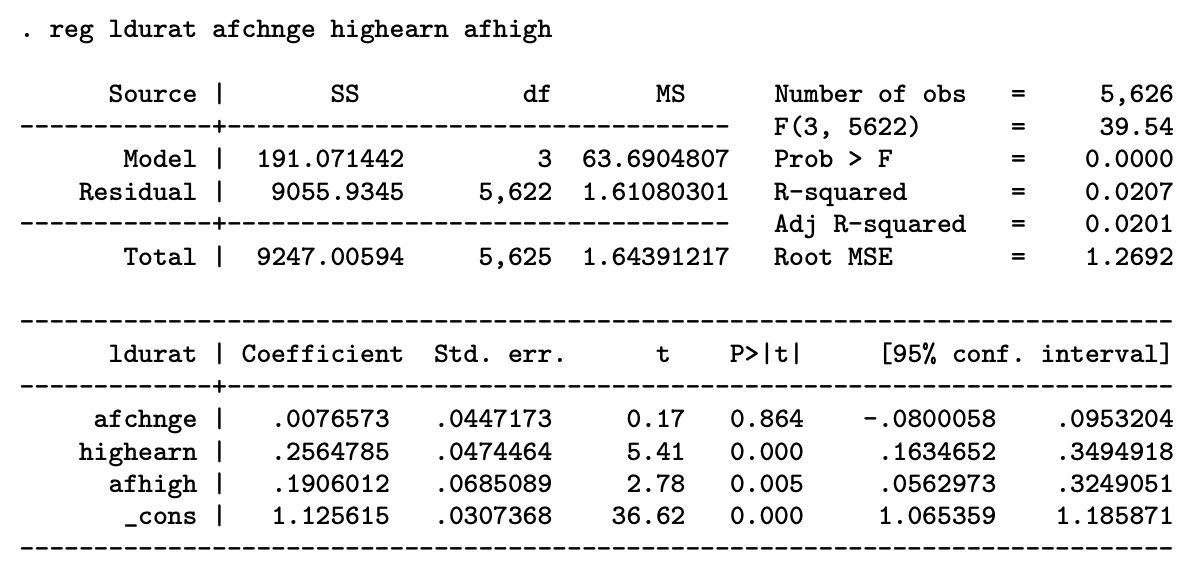
\includegraphics[width=15cm]{photos/did output.png}
        \caption{Output of the Difference in Differences Regression}
        \label{fig:DID output}
    \end{figure}
\begin{mdframed}  
    The \lstinline{afhigh} coefficient shoes that the policy increased high earners' leave duration by 19.1\%.
\end{mdframed}

\paragraph{Controls} can be added to out simple DID specification. Maybe the control and treatment group differ in multiple ways and to control for this we can include control variables.

For example, low-wage earners may experience injuries at a younger age than high-wage earners. As a result, low-wage earners require a shorter recovery period. So we can control for age at injury.

\paragraph{Multiple Groups} can be implemented to control for other issues. Maybe the control and treatment groups are trending at different rates, but nothing to do with the treatment.

In our workers' compensation example what if high earners are taking up more compensation than low earners irrespective of the policy change? \hl{We could use high earners from a different state as a second control group}. The resulting estimator is a triple difference estimator.

\paragraph{The General Approach} to policy analysis is to include multiple control and treatment groups as well as more than two time periods. We control for aggregate time effects to all groups, fixed effects specific to each group, group-specific time trends, and explanatory variables measures at the individual and group levels.

We could have some groups that are never treated, and some groups that are treated at different time periods. We could even see some groups treated, but later in the study, the treatment stops. Because of this, we could introduce a new subscript $i$ for each individual/household/firm, along with $g$: group and $t$: time period.

Our general equation can be written:
\[y_{igt} = \lambda_t + \alpha_g + \beta x_{gt} + \boldsymbol{z}_{igt}\gamma + u_{igt}\]
with $i= 1,\ldots, N_{gt}; g= 1, \ldots, G; t= 1,\ldots, T$.

$\boldsymbol{z}_{igt}$ is shorthand for multiple explanatory variables multiplied by a coefficient. The parameters $\lambda_t$ are the aggregate time effects that capture external factors. $\alpha_g$ is the group effects, systematic differences between states that are constant across time.

This still has a fatal assumption of the parallel trend assumption. One way to relax this is to introduce group-specific linear time trends, if we have at least $T\geq 3$.

\[y_{igt} = \lambda_t + \alpha_g + \psi_g t + \beta x_{gt} + \boldsymbol{z}_{igt}\gamma + u_{igt}\]




\paragraph{Continuous Variables} can be used is the treatment is not binary. For example, if the policy increased compensation proportionally to earnings (a continuous treatment) rather than raising the earnings cap (a binary treatment), we could use a treatment of log earnings and set up the regression as normal. We would still have an interaction term, but it would be a continuous variable, log earnings, and the time indicator, binary.



\subsection{Simple Panel Data Analysis}

Panel data follows the same units (individuals, households, firms etc.) over two or more periods.

\hl{Pooled cross sections have different sampled units in each period}. The main benefit of panel data is with multiple years we can control for unobserved characteristics that do not change over time. This is useful for policy analysis.

\paragraph{Balanced Panels} are panel data sets where we observe the same time periods for each unit. This tends to be much easier for larger units like schools and cities.

\begin{shaded}
    \paragraph{Notation:} \mbox{}

    For each cross-sectional unit $i$ at time $t$ the response variable is $y_{it}$, explanatory variable is $x_{it}$. 

    When we have more than one explanatory variable we have $x_{it1}, x_{it2}, \ldots, x_{itk}$.

    Unobserved effects or \textit{unobserved heterogeneity} $a_i$ which changes between individuals but not time, i.e. innate ability.

    $u_{it}$ are the idiosyncratic errors, sometimes called shocks. Specific to unit $i$ and vary over time, affecting the final outcome $y_{it}$.
\end{shaded}



\paragraph{Long Format Panel Data} is the most common format for storing panel data. It is when the time periods for each unit are adjacent and stored in chronological order. 
\begin{mdframed}
    we would use the command \lstinline{xtset id term}, to declare our data set to be panel data. Where id=$i$ and term=$t$.
\end{mdframed}

\paragraph{Wide Format Panel Data} is sometimes seen with data sets of two years. We will only have $n$ records, rather than $2n$ with two year long format. Variables from different years need different suffixes. This all makes it much harder to work with especially if there are more than two years.
\begin{figure}[h]
    \centering
    \subfloat[\centering Long Format Panel Data]{{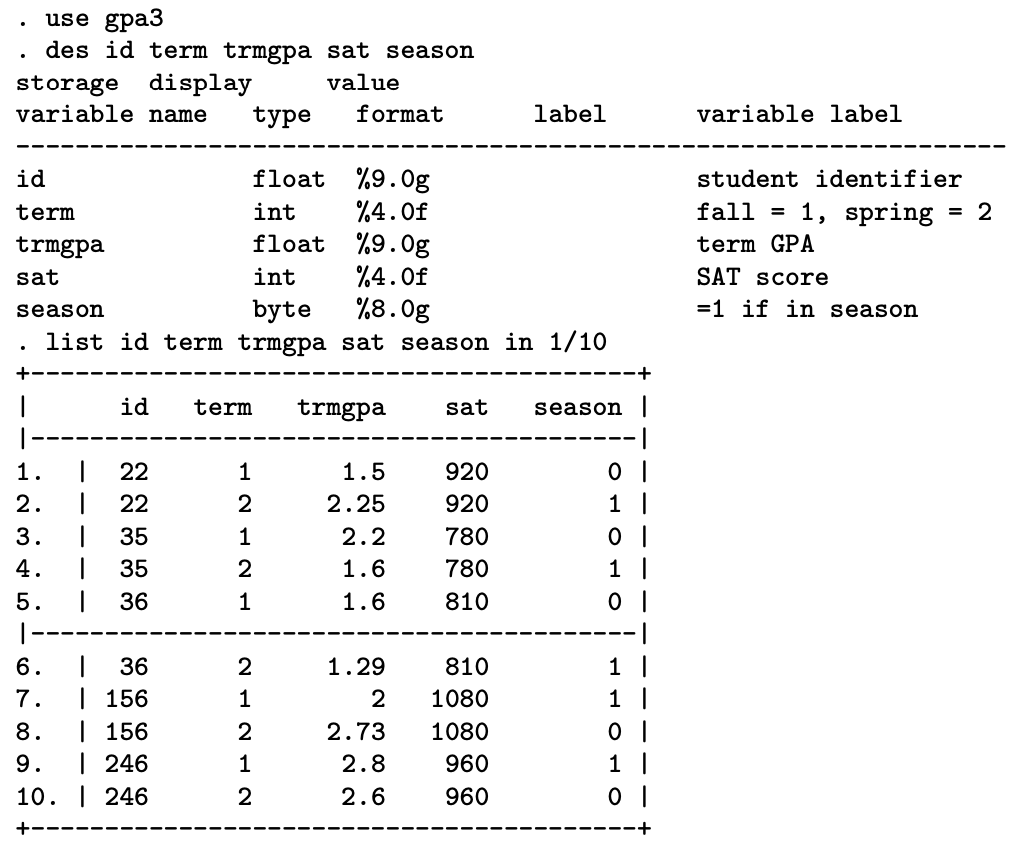
\includegraphics[width=7cm]{photos/long format.png} }}%
    \qquad
    \subfloat[\centering Wide Format Panel Data]{{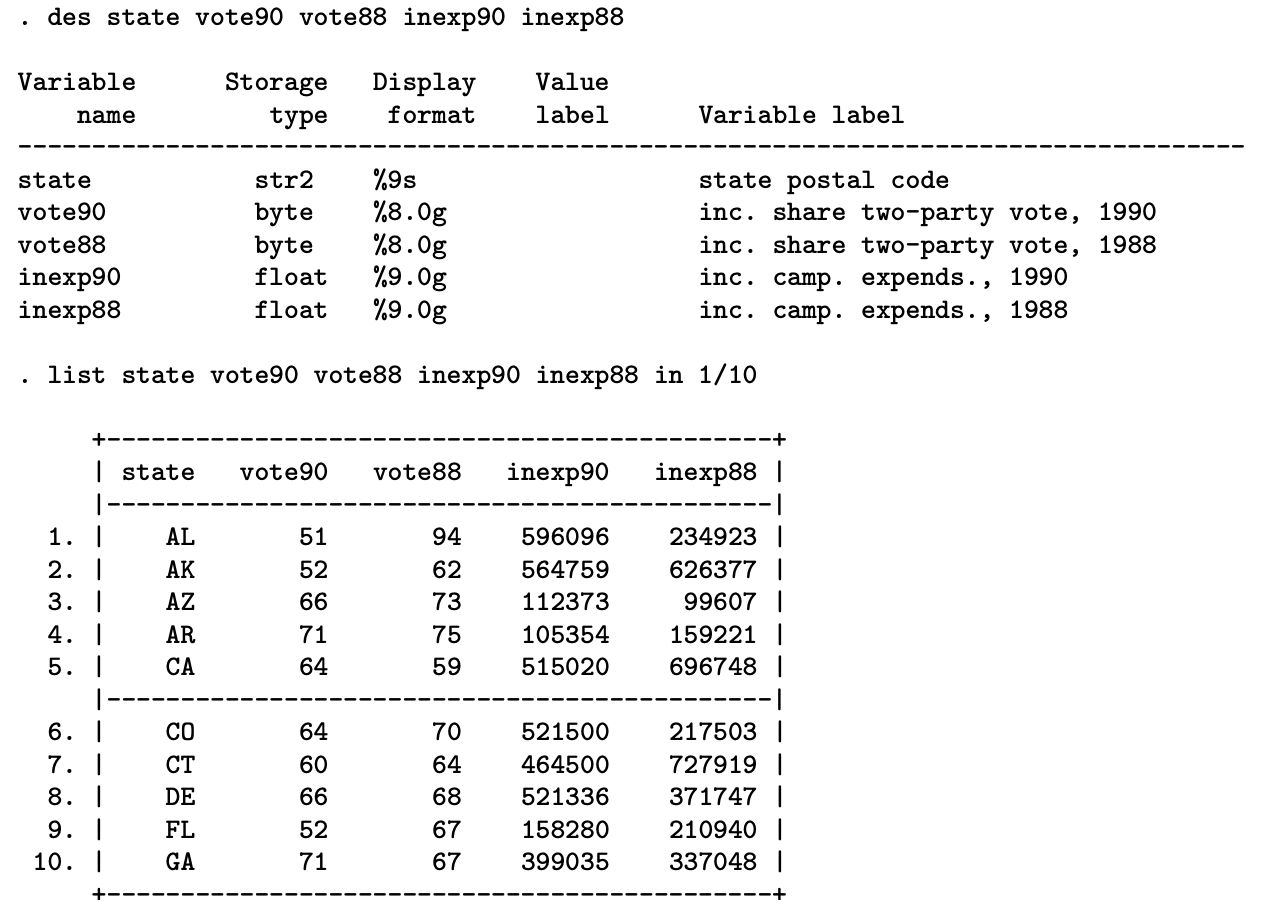
\includegraphics[width=7cm]{photos/wide panel.png} }}%
    \caption{Different Formats of Panel Data}%
    \label{fig:panel format}%
\end{figure}


\subsubsection{2 period model}

The equation is:
\begin{equation}
    \label{panel simple model}
    y_{it} = \beta_0 + \delta_0 d2_t + \beta_1 x_{it} + a_i + u_{it}, \quad t=1,2.
\end{equation}

We observe $x_{it}, y_{it}$ for each of the two time periods. $d2_t$ is an indicator variable for the second time period. As mentioned earlier $a_i$ is the unobserved unit effect and $u_{it}$ is the unobserved idiosyncratic error.

We are interested in estimating $\beta_1$, the partial effect of $x$ in $y$. We are implicitly assuming that this effect is constant over time.

$\beta_0$ is the intercept in the first period and $\beta_0 + \delta_0$ is the intercept in the second period. It is important to allow for changing intercepts to get a good estimate of a causal effect.

One requirement for the consistency of OLS is that $cov(x_{it},a_i) = 0$. When this is violated we have \textbf{heterogeneity bias}. We often see this in pooled OLS. If the explanatory variable changes over time - even just for some units in the population - heterogeneity bias can be solved by differencing away $a_i$.

\subsubsection{Differencing 2 period model}

We have each period's estimation equation:
\begin{align}
 y_{i2} &= (\beta_0 + \delta_0) + \beta_1 x_{i2} + a_i + u_{i2} \\
 y_{i1} &= \beta_0 + \beta_1 x_{i1} + a_i + u_{i1}
\end{align}

By subtracting period 1 from period 2 we get:
\begin{equation}
    y_{i2} - y_{i1} = \delta_0 + \beta_1(x_{i2} - x_{i1}) + (u_{i2} - u_{i1}).
\end{equation}

This can be rewritten as 
\begin{equation}
    \label{differenced two period panel}
    \Delta y_i = \delta_0 + \beta_1 \Delta x_i + \Delta u_i
\end{equation}

This is called the \textbf{First-Difference estimator}, (FD estimator). We still have $\beta_1$, the original coefficient of interest. Now the intercept is just $\delta_0$, the change in the intercept over the two time periods. If $x_{it}$ is constant over time for all $i$, this strategy does not work. We need some within-unit variation for this method to work.

\subsubsection{General FD estimation}

When we have more than 2 periods of panel data, we must be careful for serial correlation in the FD equation. This is because the FD equation \hl{is no longer just a single cross section}. We tend to include a full set of time indicator variables.

\begin{mdframed}
    \paragraph{The Model} \mbox{}

    With $T$ time periods, where now $T\geq2$, we can write

    \begin{equation}
    \label{panel general model equation}
y_{i t}=\delta_1+\delta_2 d 2_t+\ldots+\delta_T d T_t+\beta_1 x_{i t 1}+\beta_2 x_{i t 2}+\ldots+\beta_k x_{i t k}+a_i+u_{i t}
\end{equation}
where $\delta_t$ is the difference between the intercept in period $t$ and period 1. Obviously, this model still contains our unobserved heterogeneity, $a_i$.


The model after differencing:

\begin{equation}
    \Delta y_{it} = \delta_2 \Delta d2_t + \delta_3 \Delta d3_t + \ldots + \delta_T \Delta dT_t + \beta_1 \Delta x_{it1} + \ldots + \beta_k \Delta x_{itk} + \Delta u_{it}
\end{equation}
Interestingly we have \textit{differenced time indicator variables}. These behave in a very strange way. Because $d2_t$ is a dummy variable for when we are in time 2, we can interpret $d2_{t-1}$ as a dummy variable which is equal to 1 when it was period 2 in the last period i.e. period 3. $d2_{t-1} = d3_t$. Our intercept has been differenced away, which is inconvenient for computing $R^2$. Because of these two inconveniences, it can be easier to difference the explanatory variables and $y_{it}$ but leave the time indicators alone. We will lose one of the time indicators simply from differencing. 

We are left with:
\begin{equation}
\label{FD panel general}
\Delta y_{i t}=\alpha_0+\alpha_3 d 3_t+\ldots+\alpha_T d T_t+\beta_1 \Delta x_{i t 1}+\beta_2 \Delta x_{i t 2}+\ldots+\beta_k \Delta x_{i t k}+\Delta u_{i t}
\end{equation}

\end{mdframed}

Our Equation \eqref{FD panel general}, is an \textit{estimation equation} to get rid of $a_i$. \hl{We need to interpret in the context of the original \textbf{levels} equation} \eqref{panel general model equation} . 

\paragraph{Extensions:} \mbox{}

From our starting equation \eqref{panel general model equation}, it is easy to choose explanatory variables for policy evaluation that allow for things like lagged results. We can also include quadratics and interactions. This is all done before differencing.

\subsubsection{Policy Analysis with Panel Data}

We can include a binary indicator to tell us once an intervention/policy has been put in place.

\begin{equation}
y_{i t}=\eta_1+\alpha_2 d 2_t+\ldots+\alpha_T d T_t+\beta \boldsymbol{w_{it}}+ \boldsymbol{x_{it}} \psi+a_i+u_{i t}, t = 1,\ldots, T
\end{equation}

$\boldsymbol{x_{it}}$ is just shorthand for the vector of explanatory variables. And $\boldsymbol{w_{it}}$ is the binary intervention indicator, while $\beta$ estimates the average treatment effect of the policy.

To allow $w_{it}$ to be systematically related to the unobserved heterogeneity $a_i$, we will estimate this using either first differencing (FD) fixed effects (FE). We can also include lags of $w_{it}, w_{it-1}$.


\newpage
\section{Advanced Panel Data Methods}

The advanced panel methods that we look at are fixed effects, random effects, and correlated random effects estimation techniques.

\subsection{Fixed Effects Estimation}
An alternative to first differencing to remove the unobserved effects is to use fixed effects estimation (within transformation).

Our simple model with unobserved effects:
\[y_{it} = \beta_1 x_{it} + a_i + u_{it}, \quad i = 1,\ldots, N, \quad t = 1,\ldots, T\]
 For each $i$ we average our equation over time, we get:
 \[\Bar{y}_i = \beta_1 \bar{x}_i + a_i + \bar{u}_i,\]
 where $\bar{y}_i = \frac{1}{T}\sum_{t=1}^T y_{it}$. Because $a_i$ is fixed over time it appears in both our original equation and our averaged equation. If we subtract our averaged equation from our original equation we get:

 \[y_{it} - \bar{y}_i = \beta_1 (x_{it} - \bar{x}_i) + u_{it} - \bar{u}_i,\]

 which can be rewritten as:
 \begin{equation}
     \label{first difference base equation}
     \Ddot{y}_{it} = \beta_1 \Ddot{x}_{it} + \Ddot{u}_{it}, \quad t=,1,2,\ldots,T
 \end{equation}
 where $\Ddot{y}_{it} = y_{it} - \bar{y}_i$ is the \textbf{time demeaned data}. \hl{This is called the within transformation or the fixed effects transformation.}

 \begin{example}
 If we were to look at the relationship between crime and unemployment with a dataset with many different cities we may find results that do not show to the true relationship between the variables, but rather find the relationship between cities.
 \end{example}
\begin{figure}[ht]
    \centering
    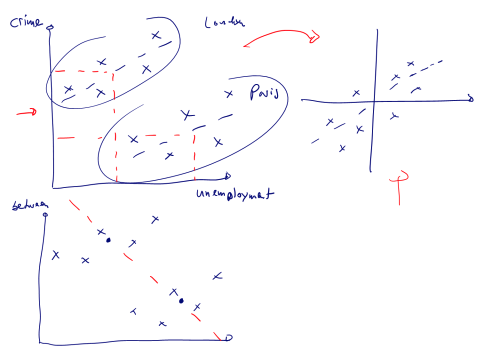
\includegraphics[width=9cm]{photos/fixed effects diagram.png}
    \caption{Process of time demeaning the data}
    \label{fig:fixed effects diagram}
\end{figure}


\begin{example}
    Consider a simple wage equation based on two waves of UK panel data from Understanding Society:
    \[lwage_{it} = \beta_0 + \beta-1 age_{it} + \beta_2 age^2_{it} + \beta_3 maried_{it} + \beta_4 yrschool_{it} + \beta_5 w2_{it} + a_i + u_{it}\]

    We can estimate this by POLS and ignore $a_i$ or use the within transformation to get:
    
    \[\Ddot{lwage}_{it} = \beta_2 \Ddot{age}^2_{it} + \beta_4 \Ddot{married}_{it} + \beta_5 \Ddot{w2}_{it} + \Ddot{u}_{it}\]

    \begin{note}
        this transformation gets rid of $a_i$ but also age and years of schooling because:
        \[\Ddot{age}_{i1} = -0.5, \Ddot{age}_{i2} = 0.5, \Ddot{yrschool}_{i1} = 0, \Ddot{yrschool}_{i2} = 0\]
    \end{note}

\end{example}

\begin{figure}[h]
    \centering
    \subfloat[\centering Initial Data for Estimation]{{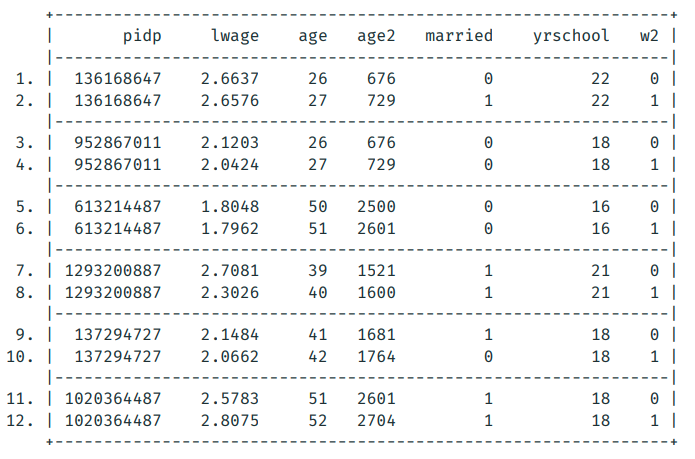
\includegraphics[width=7cm]{photos/fixed effects first table.png} }}%
    \qquad
    \subfloat[\centering After Within Transformation ]{{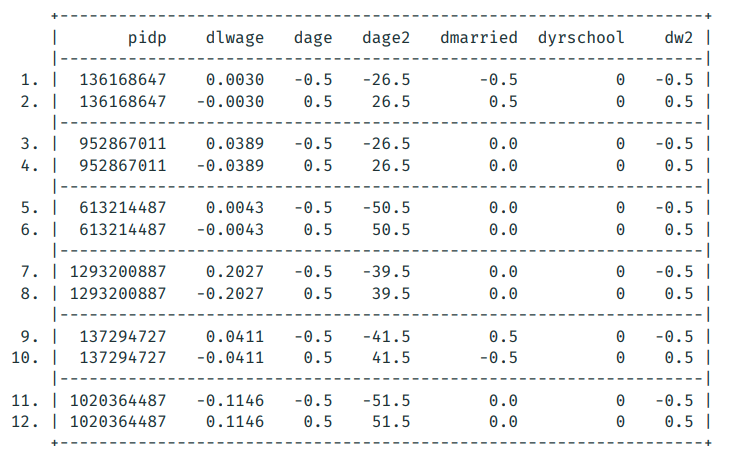
\includegraphics[width=7cm]{photos/fixed effects after transformation table.png} }}%
    \caption{Pre- and Post-Transformation}%
    \label{fig:fe example}%
\end{figure}


\begin{figure}[h]
    \centering
    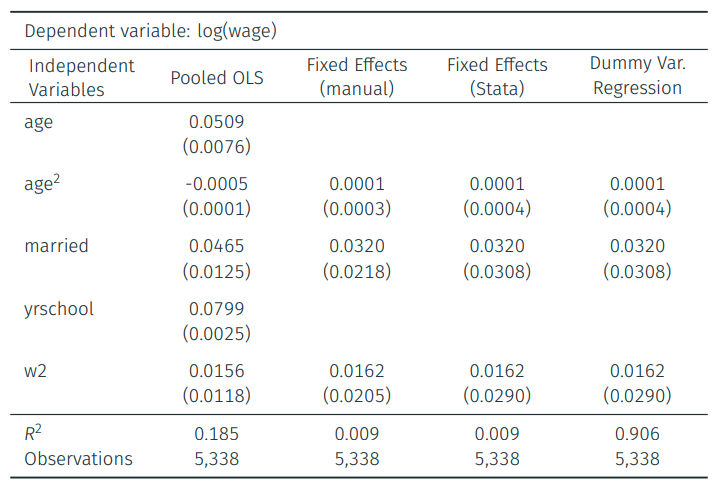
\includegraphics[width=10cm]{photos/fe example results.png}
    \caption{Results from the POLS, FE and manual FE, and Dummy Variable Regression}
    \label{fig:fe example results}
\end{figure}

\subsubsection{Assumptions for FE}

\begin{itemize}
    \item [FE.1] For each $i$ the model is:
    \begin{equation}
y_{i t}=\beta_1 x_{i t 1}+\ldots+\beta_J x_{i t\rfloor}+\delta_2 d 2_t+\ldots+\delta_T d T_t+a_i+u_{i t}
\end{equation}
This means that we have \textbf{linear parameters}
\item [FE.2] We have a \textbf{random sample} from the cross-section
\item [FE.3] Each explanatory variable changes over time, and \textbf{no perfect linear relationships} exist among the explanatory variables.
\item [FE.4] $E(u_{it}|\boldsymbol{X}_i, a_i) = 0 \Rightarrow x$ is uncorrelated with $u$ for all time periods conditional on $a_i$, \textbf{strict exogeneity}. 
\item[FE.5] \textbf{Homoskedasticity} $\Rightarrow Var(u_{it}|\boldsymbol{X}_i,a_i) = \sigma_u^2$
\item [FE.6] \textbf{No serial correlation}: $\Ddot{u}_{it}$ is uncorrelated over time $\Rightarrow Cov(u_{it},u_{is}|\boldsymbol{X}_i, a_i) = 0 ]forall
t\neq s$
\end{itemize}


\begin{note}
    FE.1-FE.4: Fixed effects is \textbf{unbiased} and \textbf{consistent} as $N \rightarrow \infty$ and $T$ is fixed.

    FE.1-FE.6: Fixed effects is \textbf{BLUE}.
\end{note}

FE.4: Strict exogeneity means that current shocks, $u_{it}$, are uncorrelated with independent variables $(x_{it1},\ldots, x_{itj})$ for \textbf{every period}.

This implies that no omitted lagged effects are present, but lagged variables can be included in $x$. Also there is no feedback from $u$ to future $x$. If strict exogeneity fails, the fixed effects estimator is not unbiased nor consistent.

\subsubsection{Fixed Effects vs First Difference}

Fixed Effects is a powerful method to deal with the problem of unobserved heterogeneity if $a_i$ appears in the model for $y_{it}$ and
\[cov(a_{i},x_{itj}) \neq 0, \text{ and } E(u_{it}|\boldsymbol{X}_i,a_i)=0\]

\begin{note}
    FE.1-FE.4 is equivalent to FD.1-FD.4, meaning both are unbiased and consistent as $N\rightarrow\infty$.
\end{note}

For $T=2$ FE and FD are identical. For $T\geq 3$ it is a question of which is more efficient. This can be seen in their final two assumptions, as this is where the estimators differ.

\newpage
\paragraph{Assumptions 5/6:} \mbox{}

\begin{itemize}
    \item [FE.5] $var(u_{it}|\boldsymbol{X}_i, a_i) = \sigma_u^2, \forall t$
    \item [FE.6] $cov(u_{it},u_{is}|\boldsymbol{X}_i,a_i)=0, \forall t \neq s$
    \item [FD.5] $var(\Delta u_{it}|\boldsymbol{X}_i) = \sigma^2$
    \item [FD.6] $cov(\Delta u_{it}, \Delta u_{is} | \boldsymbol{X}_i) = 0, \forall t \neq s$
\end{itemize}

\hl{FE is more efficient when errors are serially uncorrelated}. FE is more efficient when errors are strongly serially correlated (random walk).

Since we never know for sure which assumption is better it is a good idea to estimate both FD and FE and see how different the results are. 

\paragraph{Post Estimation Analysis} \mbox{}

After we have conducted our FD estimation we can test for serial correlation in the differenced errors. First estimate FD, and calculate the residuals. Let:
\[r_{it} = \Delta u_{it}\]
Then we run a Pooled OLS of $\hat{r}_{it} on \hat{r}_{it-1} \Rightarrow \hat{\rho}$.

$\hat{\rho}$ is the estimated correlated coefficient of the estimated residual on its lag. (these are residuals obtained from the FD estimation). If we see no serial correlation in the differenced errors, $r_{it} = \Delta u_{it}$, then we know that there must have been a unit root in our non-differenced error terms. In this case FD is more efficient, due to FD.6: No serial correlation in the difference errors
\[cov(\Delta u_{it}, \Delta u_{is} | \boldsymbol{X}_i) = 0, \forall t \neq s.\]

\begin{note}
With standard data most of the literature has settled on FE with cluster-robust standard errors.    
\end{note}

\subsubsection{Fixed Effects with Unbalanced Data}

If the panel is unbalanced, i.e. we have missing observations for some $i,t \rightarrow \sum_i^N t_i <N\times T$. 

As long as all $T_i$ are large enough, the fixed effects procedure is still valid. But we should be worried about why it's unbalanced, Are observations missing at random or is there selective attrition?

\subsubsection{Application of FE}

    The effect of school quality on student outcomes (Autor et al., 2016)

Interested in the differential effect of school quality on girls and boys. Motivating evidence:
\begin{itemize}
    \item Women have higher eduaction than men in most countries in recent years
    \item e.g. in the US female high school graduation rate is 5\% larger than men's
    \item One potential driver is that girls benefit more from school quality
\end{itemize}

We look at standardised maths and reading scores, absenteeism rates, the incidence of school suspension. School Quality: value added measured by the Florida Department of Education, average between 2002-2013 converted into a rank. Each student hets a cumulative quality of school attended (weighted average of school quality).

\begin{table}[h]
    \centering
    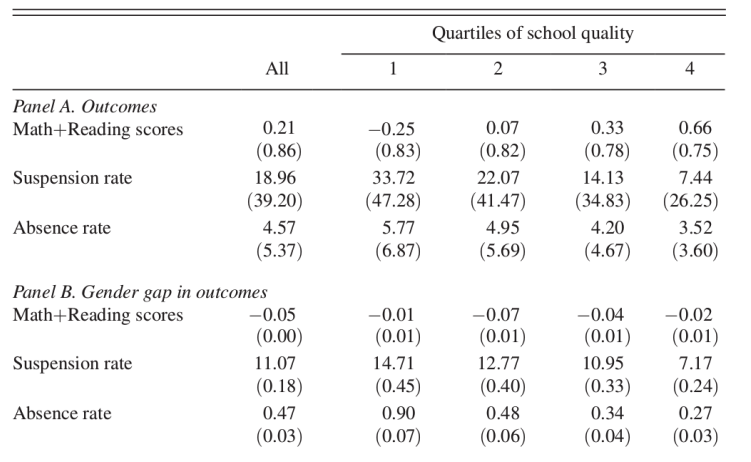
\includegraphics[width=10cm]{photos/fe application sum stats.png}
    \caption{Summary Statistics in Autor et al., 2016}
    \label{tab:fe summary stats}
\end{table}

\begin{figure}[h]
    \centering
    \subfloat[\centering Outcome A: Standardised scores against School Quality]{{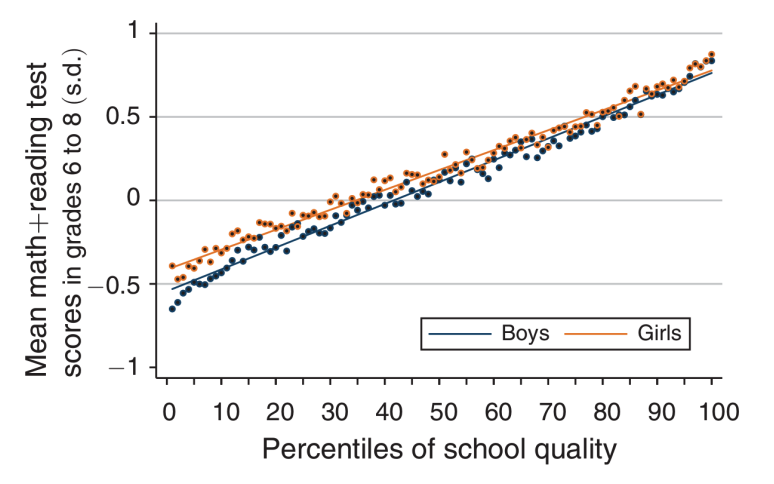
\includegraphics[width=7cm]{photos/fe score vs quality.png} }}%
    \qquad
    \subfloat[\centering Outcome B: Suspension Rate vs School Quality]{{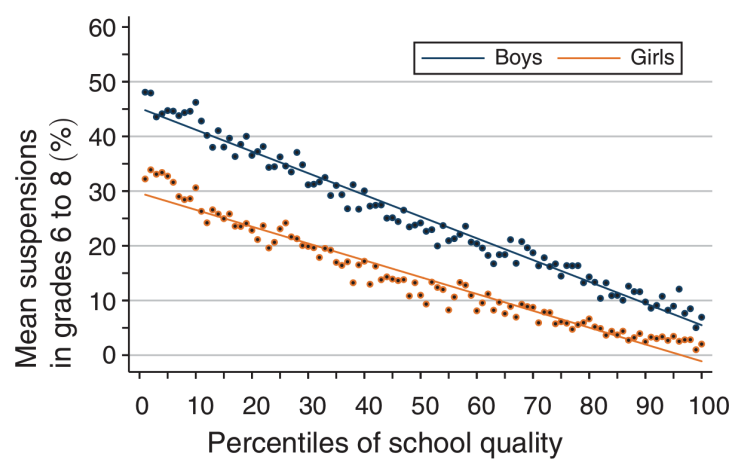
\includegraphics[width=7cm]{photos/fe suspensions vs quality.png} }}%
    \caption{Sample statistics against School Quality}%
    \label{fig:fe application diagrams}%
\end{figure}

The main concern we have here is unobserved heterogeneity. Are bots who attend lower-quality schools already disadvantaged relative to girls OR are boys more sensitive to the academic/disciplinary environment?

We can compare siblings \textbf{within} families. The estimate:
\begin{equation}
y_{i j}=\beta_0+\beta_1 Q_{i j}+\beta_2 B_0 y_i+\beta_3\left(B_0 y_i * Q_{i j}\right)+\boldsymbol{\delta} F_{i j}+\boldsymbol{\mu} X_i+\gamma_j+\varepsilon_{i j}
\end{equation}

where $y_{ij} \equiv$ outcome for child $i$ in family $j$, $Q_{ij} \equiv$ quality of school attended by child $i$ in family $j$, $Boy_i \equiv$ child is a boy, $\boldsymbol{F}_{ij} \equiv$ family/child characteristics (e.g. maternal education at child's birth), $\boldsymbol{X}_i \equiv$ child characteristics (e.g. month and year of birth, birth order), $\gamma_i$ family (mother) \textbf{fixed effect}.

\begin{table}[h]
    \centering
    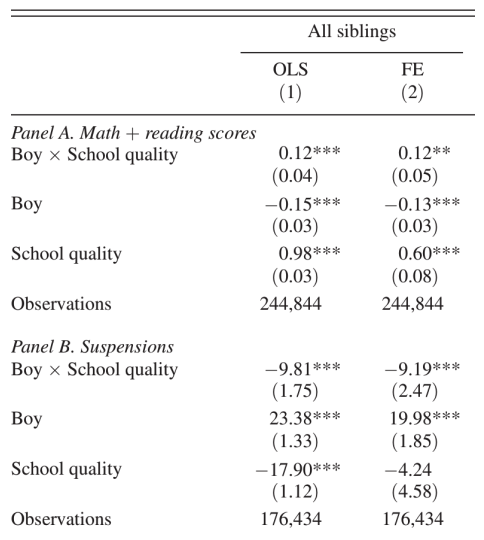
\includegraphics[width=10cm]{photos/fe application results.png}
    \caption{Results of the Study, Comparing POLS and FE}
    \label{tab:fe application results}
\end{table}


\subsection{Random Effects}

The unobserved effect model:
\begin{equation}
y_{i t}=\beta_0+\beta_1 x_{i t 1}+\ldots+\beta_{\jmath} x_{i t)}+a_i+u_{i t}
\end{equation}
Here we assume that $cov(a_i,x_{itj}) = 0 \forall j,t$. $a_i$ is uncorrelated with all explanatory variables for all periods. This means it is inefficient to eliminate $a_i$. Under this assumption, there is a more efficient estimator, \textbf{Random Effects}.

Let the composite error term be $v_{it} = a_i + u_{it}$. This gives us:

\[y_{i t}=\beta_0+\beta_1 x_{i t 1}+\ldots+\beta_{\jmath} x_{i t)}+v_{it}\]

where $v_{it}$ is correlated over time:
\begin{equation}
\operatorname{Corr}\left(v_{i t}, v_{i s}\right)=\frac{\sigma_a^2}{\sigma_a^2+\sigma_u^2}, t \neq s
\end{equation}
where $var(a) = \sigma_a^2$ and $var(u) = \sigma_u^2$. This correlation would not be taken into account in the POLS.

Let $\theta=1-\left(\dfrac{\sigma_u^2}{\sigma_u^2+T\sigma_a^2}\right)^{1/2}$

then we have
\begin{equation}
y_{i t}-\theta \bar{y}_i=\beta_0(1-\theta)+\beta_1\left(x_{i t 1}-\theta \bar{x}_{i 1}\right)+\ldots+\beta_{\jmath}\left(x_{i t t}-\theta \bar{x}_{i j}\right)+\left(v_{i t}-\theta \bar{v}_i\right)
\end{equation}

If $v_{it} - \theta\bar{v}_i$ is uncorrelated over time we use POLS. With this \textbf{quasi-demeaned} data, the Random Effects does not require $x_i$ to change over time.

\begin{note}
    If $\theta\rightarrow0\Rightarrow$ RE converges to POLS. If $\theta\rightarrow1\Rightarrow$ RE converges to FE.
\end{note}

$\theta$ is usually not known in practice. It depends on the error variances $\sigma_{a}^2, \sigma_u^2$. $\hat{\sigma}_{a}^2, \hat{\sigma}_u^2$ can be based on POLS or FE. Using $\hat{\theta}$ we can implement \textbf{feasible GLS}. This FGLS procedure is called the Random Effects estimator.
\begin{definition}
\subsubsection{RE Assumptions}

$\hat{\beta}^{RE}$ is consistent under:
\begin{itemize}
    \item FE.1 FE.2 FE.4
    \item RE.1: There are no perfect linear relationships among the explanatory variables
    \begin{note}
        This differs from FE.3 and FD.3 as we are not assuming that each explanatory variable changes over time.
    \end{note}
    \item RE.2: $E(a_i|\boldsymbol{X}_i)=\beta_0$. This implies that the covariance between the unobserved heterogeneity and our explanatory variables is 0: $cov(a_i, \boldsymbol{X}_i)=0$
\end{itemize}

It is also asymptotically efficient if we add \textbf{homoskedasticity:}
\begin{itemize}
    \item FE.5 $var(u_{it}|\boldsymbol{X}_i,a_i)=\sigma_u^2$
    \item RE.3 $var(a_i|\boldsymbol{X}_i)=\sigma_a^2$
\end{itemize}
\end{definition}



\subsubsection{Random Effects vs Fixed Effects}

FE has an advantage in that correlation between our unobserved heterogeneity, $a_i$, and our explanatory variables, $x_{itj}$, is allowed. RE has an advantage in that we can include variables that do not vary over time e.g. education.

In practice we can apply both RE and FE and test for differences in coefficients on time-varying $x$.

\paragraph{Hausman Test}

The Hausman Test tests whether we should use Fixed Effects or Random Effects:
\begin{itemize}
    \item Use FE if $H_0: corr(z_i,x_{itj}) = 0$ is \textbf{rejected}.
    \item If $H_0$ is not rejected it is probably safe to use RE.
\end{itemize}


\subsection{Correlated Random Effects}
In some applications, it makes sense to think of $a_i$ as a random variable:
\[a_i = \alpha + \gamma \bar{x}_i + r_i.\]

We assume that:
\begin{itemize}
    \item $cov(r_i,x_{it})=0$
    \item $cov(u_{it}, x_{it}) = 0 \rightarrow cov(i_i, \bar{x}_i) = 0$
\end{itemize}

Our equation for $a_i$ can be substituted into our Fixed Effects, our simple model with unobserved effects:
\[y_{it} = \alpha + \beta x_{it} + \gamma \Bar{x}_{it} + r_i + u_{it}\]

 We now have an RE with uncorrelated random effects $r_i$ and time averages, $\Bar{x}_i$ as additional regressors. $\hat{\beta}^{CRE} = \hat{\beta}^{FE}$.

 Why would we use CRE? $\hat{\gamma}$ is used to test RE vs FE. Additionally, it can incorporate time-invariant regressors.

 \subsection{Other Data Structures}

 These methods can be used for a variety of data structures, not only individuals over time.

 \begin{itemize}
     \item Matched pairs samples - twins to control for family background
     \item Cluster samples - cluster is a well-defined group of individuals. Clusters of units are sampled from a population of clusters. Cluster samples are cross-sectional data, but made of well-defined groups. We need variation within clusters. 

    \item Examples - individuals born in a given year, pupils in a given class.
 \end{itemize}


\section{instrumental Variables}

\subsection{The Instrumental Variable Estimator}

The instrumental variable (IV) estimation method helps with the problem of endogenous explanatory variables. OLS is consistent iff. exogeneity holds.
\begin{example}
    The simple one-regressor case:
    \[y_i = \beta_0 + \beta_1 x_i + u_i\]
    Exogeneity implies
    \begin{align*}
        cov(x_i,u_i)&=0 \\
        cov(x_i, y_i - \beta_0 - \beta_1 x_i) &= cov(x_i, y_i) - \beta_1 var(x_i) = 0 \\
        \beta_1 &= \dfrac{cov(x_i,y_i)}{var(x_i)}
    \end{align*}
\end{example}

Our motivation for instrumental variables can be seen in the case of OVB in a simple regression.
\begin{definition}
    Consider
\[y = \beta_0 + \beta_1 x + u\]
assume that there is an instrument $z$ s.t.
\begin{itemize}
    \item \textbf{Instrument Relevance}: $cov(z,x) \neq0$
    \item \textbf{Instrument Exogeneity}: $cov(z,u)=0$
\end{itemize}
These assumptions identify the parameter $\beta_1$:
\begin{equation}
\begin{aligned}
\operatorname{Cov}(z, y) & =\beta_1 \operatorname{Cov}(z, x)+\operatorname{Cov}(z, u) \\
\beta_1 & =\frac{\operatorname{Cov}(z, y)}{\operatorname{Cov}(z, x)}
\end{aligned}
\end{equation}
We can estimate population moments with sample moments
\begin{equation}
\label{IV estimator}
\hat{\beta}^{IV} =\frac{\widehat{\operatorname{Cov}(z, y)}}{\widehat{\operatorname{Cov}(z, x)}}
\end{equation}
\end{definition}


\begin{example}
    We are assessing the effect of education on wages with unobserved ability that is correlated with wages and education
    \[log(wage) = \beta_0 + \beta_1 educ + \beta_2 abil + e\]

    If we ignore ability and run OLS we have the ability in the error term: $u = \beta_2 + e$. This is called a \textbf{composite error}.
    \[log(wage) = \beta_0 + \beta_1 educ + u\]

    From our data we get:
    \[log(wage) = -\underset{(0.185)}{0.185} + \underset{(0.014)}{0.109}educ\]

    OLS is biased and inconsistent:
    \begin{equation}
\begin{aligned}
\operatorname{Cov}(\text { educ }, u) & =\operatorname{Cov}\left(\text { educ }, \beta_2 \text { abil }+e\right) \\
& =\beta_2 \operatorname{Cov}(\text { educ }, \text { abil }) \neq 0
\end{aligned}
\end{equation}

If we use father's education as an instrument, we may use this as a proxy for innate ability. We must assume instrument exogeneity and instrument relevance (it is strongly correlated with educ so this is okay).

\[educ = \underset{(0.28)}{10.24} + \underset{(0.029)}{0.269}fatheduc\]

Now using this estimated value of education we can estimate using IV with the father's education as an instrument:
\[log(wage) = \underset{(0.446)}{0.441} + \underset{(0.035)}{0.059}educ\]

The reason for the change in estimation is because in our first estimation:
\begin{align*}
    \underset{N\rightarrow\infty}{plim} \hat{\beta}_1 &= \beta_1 + \dfrac{cov(educ,u)}{var(educ)} \\
    &= \beta_1 + \dfrac{cov(educ,\beta_2 abil + e)}{var(educ)} \\
    &= \beta_1 + \dfrac{cov(educ,\beta_2 abil)}{var(educ)} + \dfrac{cov(educ,e)}{var(educ)}\\
    &= \beta_1 + \beta_2\dfrac{cov(educ,abil)}{var(educ)}
\end{align*}
We know that there is some correlation between education and ability and therefore there will be some bias to our IV estimator.
\end{example}

\subsection{Statistical Inference with the IV estimator}

Along with our previous assumptions of $u,x,z$, if we also add the homoskedasticity assumption:
\begin{equation}
E\left(u^2 \mid z\right)=\sigma^2=\operatorname{Var}(u)
\end{equation}
Then $\hat{\beta}^{IV}$ is asymptotically normally distributed (CLT)
\begin{equation}
\hat{\beta}^{I V} \stackrel{a}{\sim} N\left(\beta, \frac{\sigma^2}{n \sigma_\chi^2 \rho_{x, z}^2}\right)
\end{equation}
where $var(u) = \sigma^2, var(x) = \sigma_x^2, corr(x,z)=\rho_{x,z}$. This leads to the asymptotic standard error
\begin{equation}
\operatorname{se}\left(\hat{\beta}^{I V}\right) \approx \sqrt{\frac{\hat{\sigma}^2}{S S T_x \cdot R_{x, z}^2}}
\end{equation}
\begin{note}
    In the case where $R^2_{x,z}=1$, that is $x$ and $z$ are perfectly correlated, we get the OLS variance as expected. If they are very uncorrelated and $R^2_{x,z}$ is close to zero, we get extremely large standard errors.
\end{note}

\subsection{Different Forms of IV}

\subsubsection{IV with Additional Controls}

Consider the \textbf{structural equation}:
\begin{equation}
y_1=\beta_0+\beta_1 y_2+\beta_2 z_1+u_1
\end{equation}

Assume $y_2$ is endogenous but we have an instrument $z_2$ that does not appear in the structural equation. We can use the IV estimator to get $\hat{\beta}_1$ under \textit{slightly modified assumptions}.
\begin{shaded}
    \textbf{Modified Assumptions}:

    The first two assumptions are standard:
    \begin{itemize}
        \item $E(u_1) = 0$
        \item $cov(z_1,u_1) = 0$
    \end{itemize}

    We add instrument exogeneity:
    \begin{itemize}
        \item $cov(z_1,u_1)=0$
    \end{itemize}
    due to the presence of $z_1$ we must also add a \textbf{new} instrument relevance condition
    \begin{itemize}
        \item given
        \begin{equation}
y_2=\pi_0+\pi_1 z_1+\pi_2 z_2+v_2
\end{equation}
we must have that $\pi_2 \neq0$. This is a \textbf{reduced form equation} for $y_2$.
    \end{itemize}

    These assumptions give us moment conditions:
    \begin{gather*}
        E(u_1) = 0 \\
        E(z_1 u_1) = 0 \\
        E(z_2 u_1) = 0
    \end{gather*}
\begin{note}
    The IV estimator replaces these moment conditions with sample moments and solves for $\hat{\beta}$. This is why we sometimes refer to the IV estimator as a method-of-moments estimator.
\end{note}
\end{shaded}

\subsubsection{IV with a Binary Instrument}

This case is most simply expressed in the example of Angrist (1990) who is interested in the effect of being a veteran on earnings later in life.

\begin{example}
    Angrist (1990)

    Let $d_i \in \{0,1\}$ denote observed veteran status (treatment), and $y_i$ denote observed civilian earnings at some point in time. We'll ignore any potential controls we could add and write the structural equation as:
    \[y_i = \beta_0 + \beta_1 d_i + u_i\]

    We are worried that $cov(d_i,u_i)\neq0$. In the 1970s a national lottery randomly assigned numbers, by birth date, to young men in the US. Low numbers mean a higher chance of being drafted. Let $z_i \in \{0,1\}$ denote observed draft eligibility status where $z_i=1$ means low number and a high chance of being drafted, and $z_i = 0$ means high number.

    If the exclusion restriction, instrument relevance and exogeneity assumptions hold, then:
    \begin{equation}
\beta_1=\frac{\operatorname{Cov}\left(y_i, z_i\right)}{\operatorname{Cov}\left(d_i, z_i\right)}
\end{equation}
\end{example}

\begin{procedure}
We use the fact that $z_i$ is binary to rewrite $\hat{\beta}_1$ as a simple expression of means.
\begin{align*}
    \hat{\beta}_1&=\frac{\sum_{i=1}^n\left(z_i-\bar{z}\right)\left(y_i-\bar{y}\right)}{\sum_{i=1}^n\left(z_i-\bar{z}\right)\left(d_i-\bar{d}\right)} \\
    \hat{\beta}_1&=\frac{\sum_{i=1}^n z_i\left(y_i-\bar{y}\right)}{\sum_{i=1}^n z_i\left(d_i-\bar{d}\right)}
\end{align*}
We can rewrite the numerator as:
\begin{equation}
\sum_{i=1}^n z_i\left(y_i-\bar{y}\right)=\sum_{i=1}^n z_i y_i-\left(\sum_{i=1}^n z_i\right) \bar{y}=n_1 \bar{y}_1-n_1 \bar{y}
\end{equation}
where $n_1=\sum_{i=1}^n z_i$ is the number of observations with $z_i=1$, and we have used the fact that $\left(\sum_{i=1}^n z_i y_i\right) / n_1=\bar{y}_1$, the average of the $y_i$ over the $i$ with $z_i=1$. So far, we have shown that the numerator in $\hat{\beta}_1$ is $n_1\left(\bar{y}_1-\bar{y}\right)$. Next, write $\bar{y}$ as a weighted average of the averages over the two subgroups:
\begin{align*}
\bar{y}=\frac{n_0}{n} \bar{y}_0+\frac{n_1}{n} \bar{y}_1
\end{align*}
where $n_0 = n-n_1$. Therefore, 
\begin{equation}
\bar{y}_1-\bar{y}=\frac{n-n_1}{n} \bar{y}_1-\frac{n_0}{n} \bar{y}_0=\frac{n_0}{n}\left(\bar{y}_1-\bar{y}_0\right) .
\end{equation}
Therefore, the numerator of $\hat{\beta}_1$ can be written as:
\begin{equation}
\frac{n_0 n_1}{n}\left(\bar{y}_1-\bar{y}_0\right)
\end{equation}
By simply replacing $y$ with $d$, the denominator in $\hat{\beta}_1$ can be expressed as $\frac{n_0n_1}{n}(\bar{d}_1 - \bar{d}_0)$. When we take the ratio of these the terms involving $n_0, n_1, n$ cancel leaving us with:
\[\hat{\beta}_1 = \dfrac{\Bar{y}_1 - \Bar{y}_0}{\Bar{d}_1 - \Bar{d})_0}\]
\end{procedure}


\newpage
\begin{figure}[h]
    \centering
    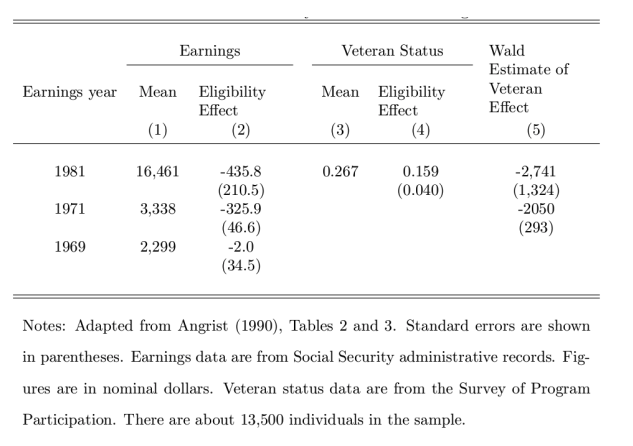
\includegraphics[width=10cm]{photos/angrist results.png}
    \caption{Wald Estimates of the effects of military service on the earnings of white mean born in 1950}
    \label{fig:angrist results}
\end{figure}
\begin{example}
    Interpretation of the Angrist Results:

    \begin{itemize}
        \item Americans with low lottery numbers had lower earnings in 1981.
        \item This suggests that serving in Vietnam had a negative effect on earnings later in life
        \item We have some concerns e.g. university to avoid the draft, which could mean that the effect of veterancy is even higher.
        \item We can test some of these concerns (but never directly the exclusion restriction/instrument exogeneity).
    \end{itemize}
\end{example}

\paragraph{The Reduced Form(s)} \mbox{}

We could of course also write down a reduced form mofrl for $y_i$
\[y_i = \delta_0 + \delta_1 z_i + v_i\]

and for veteran status (first stage):
\[d_i = \gamma_0 + \gamma_1 z_i + \eta_i\]

so:
$\bar{y}_0=\hat{\delta}_0, \quad \bar{y}_1=\hat{\delta}_0+\hat{\delta}_1, \quad \bar{d}_0=\hat{\gamma}_0, \quad \bar{d}_1=\hat{\gamma}_0+\hat{\gamma}_1$.

This illustrates that the Wald estimator "divides the reduced form by the first stage". We also call $\delta_1$ the \textbf{intention-to-treat effect}.

\paragraph{Breaking Down IV Assumptions} \mbox{}

For the intention-to-treat effect to be valid we only need $cov(z_i,v_i) = 0$, we don't need the exclusion restriction. The draft lottery is a good example where $cov(z_i,v_i) =0$ likely holds. Whether the exclusion restriction holds is a different question: people with low numbers might go to university to avoid the draft.

\subsection{Two Stage Least Squares}

Consider the structural model again:
\[y_1 = \beta_0 + \beta_1 y_2 + \beta_2 z_1 + u_1\]

suppose we have \textbf{two instrumental variables} $z_2, z_3$ excluded from out structural equation. A \textit{valid IV setup requires:}

\[E(u_1) = 0, \quad E(z_1u_1) = 0, \quad E(z_2u_1)=0,\quad E(z_3u_1)=0\]

and 
\begin{equation}
y_2=\pi_0+\pi_1 z_1+\pi_2 z_2+\pi_3 z_3+v_2
\end{equation}
where $\pi_2 \neq 0$ and/or $\pi_3 \neq0$ (relevance). \textbf{We must assume the $z_j$ are all exogenous}.

The moment conditions are:
\begin{gather*}
        E(u_1) = 0 \\
        E(z_1 u_1) = 0 \\
        E(z_2 u_1) = 0 \\
        E(z_3 u_1) = 0
    \end{gather*}

    That is 4 equations for 3 unknowns (parameter is overidentified) meaning there are many different ways of estimating $\beta_1$, we could even use the IV estimator with $z_2$ and not use $z_3$, however, this is clearly not efficient.

    What is the best way of combining the moment conditions to get estimates for the $\beta$s. The best way to get a \textit{single} instrument for $y_2$ is given by 

\begin{equation}
y_2^*=\pi_0+\pi_1 z_1+\pi_2 z_2+\pi_3 z_3
\end{equation}
which is just the reduced form for $y_2$. Given out assumptions $y_2^*$ will \textbf{not} be correlated with $u_1$. We can easily get a consistent estimate for $y_2^*$ by regressing $y_2$ on $z_1, z_2, z_3$:

\begin{equation}
\hat{y}_2=\hat{\pi}_0+\hat{\pi}_1 z_1+\hat{\pi}_2 z_2+\hat{\pi}_3 z_3
\end{equation}

This leaves us with the following equations that we solve for $\hat{\beta}_j$:
\begin{equation}
\begin{aligned}
\sum_i \hat{u}_i & =0 \\
\sum_i\left(z_{i 1} \hat{u}_i\right) & =0 \\
\sum_i\left(\hat{y}_{i 2} \hat{u}_i\right) & =0
\end{aligned}
\end{equation}

where $\hat{u}_i=y_{i 1}-\hat{\beta}_0-\hat{\beta}_1 y_{i 2}-\hat{\beta}_2 z_{i 1} .$

This is called \textbf{Two Stage Least Squares}(or TSLS/2SLS) necause of the procedure:
\begin{enumerate}
    \item Regress $y_2$ on the exogenous regressors and instruments to get $\hat{y}_2$
    \item regress $y_1$ on the exogenous regressors and the $\hat{y_2}$.
\end{enumerate}

\begin{note}
Some notes on TSLS:
\begin{itemize}
    \item IF we only have one instrument TSLS is the same as the IV estimator.
    \item If we do TSLS \textbf{manually} the standard errors are wrong because they ignore that $\hat{y}_2$ is estimated
    \item The $R^2$ is not very useful and can be negative
    \item The usual F-test does \textbf{not} work after TSLS.
\end{itemize}
\end{note}

\subsubsection{Error Issues}
We should not do manual 2SLS or rely on $R^2$ or do manual F-tests because there are two error terms floating around. We see this by replacing $y_2$ with the first stage:

\begin{equation}
\begin{aligned}
y_1 & =\beta_0+\beta_1 y_2+\beta_2 z_1+u_1 \\
& =\beta_0+\beta_1\left(\pi_0+\pi_1 z_1+\pi_2 z_2+\pi_3 z_3+v_2\right)+\beta_2 z_1+u_1 \\
& =\beta_0+\beta_1\left(\pi_0+\pi_1 z_1+\pi_2 z_2+\pi_3 z_3\right)+\beta_2 z_1+\underbrace{u_1+\beta_1 v_2}_{\text {composite }}
\end{aligned}
\end{equation}

This is difficult to correct. Most software does this for us.

\subsubsection{2SLS General Case}

We can have multiple endogenous variables, multiple instruments, and multiple exogenous regressors:
\[y_i=\beta_0+\beta_1 x_{i 1}+\ldots+\beta_K x_{i K}+\delta_1 w_{i 1}+\ldots+\delta_R w_{i R}+u_i\]

where
\begin{itemize}
    \item $y_i \equiv$ dependent variable
    \item $x_{ik} \equiv$ endogenous independent variables
    \item $w_{ir} \equiv$ exogenous independent variables
    \item $z_{im} \equiv$ instruments (excluded exogenous variables)
\end{itemize}

\begin{definition}
    Regression coefficients would be:
    \begin{itemize}
        \item \textbf{Exactly identified} if $M=K$
        \item \textbf{overidentified} if $M>K$
        \item \textbf{underidentified} if $M<K$
    \end{itemize}
\end{definition}

\begin{shaded}
    \subsubsection{2SLS Assumptions}

    \begin{itemize}
        \item 2SLS.1: Linear in Parameters
        \item 2SLS.2: We have a random sample on $y, w_r, x_k, z_m$
        \begin{note}
            The "no perfect multicollinearity" condition is tricky in IV in general. We need to state this in terms of a rank condition
        \end{note}
        \item 2SLS.3:
        \begin{enumerate}
            \item [(i)] There are no perfect linear relationships between the instrumental variables and exogenous regressors
            \item [(ii)] the rank condition for identification holds (we are not under-identified and we must have instrument relevance)
        \end{enumerate}
        \item 2SLS.4: The error term $u$ has a zero mean, and each IV/exogenous regressor is uncorrelated with $u$.
    \end{itemize}

    Under 2SLS.1-4 the 2SLS estimator is consistent.
\end{shaded}

\begin{example}
    Returning to the Wage example:

    We will add an additional instrument, the mother's education. 
    
    \begin{procedure}
    \begin{enumerate}
        \item Regress education on the exogenous variables (experience) and parent's education.
        \item Test instrument relevance using an F test on parent's education
        \item We then predict the fitted values of education and use them in the regression for log wages
    \end{enumerate}
    \end{procedure}
\end{example}

\begin{figure}[h]
    \centering
    \subfloat[\centering Regressing education on exogenous variables and parents' education]{{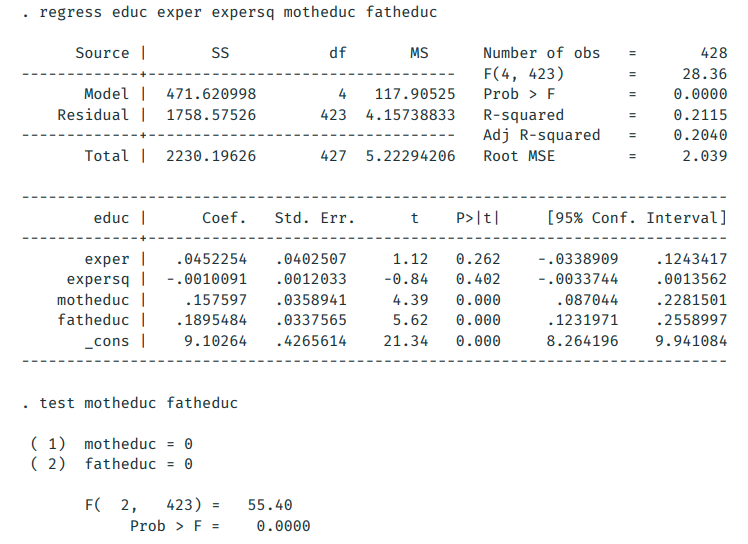
\includegraphics[width=7cm]{photos/2sls example 1.png} }}%
    \qquad
    \subfloat[\centering Predicting values and regressing]{{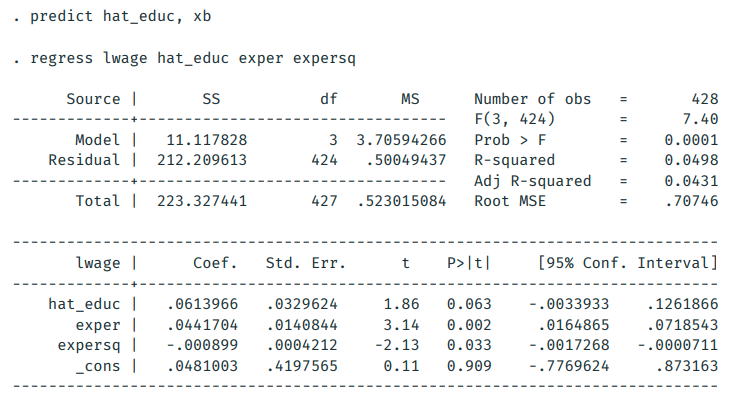
\includegraphics[width=7cm]{photos/2sls 2nd stage.png} }}%
    \caption{Example of 2SLS in STATA}%
    \label{fig:2sls example}%
\end{figure}

\begin{example}
Results:

Instrument relevance clearly holds from the F-test. We get a barely significant coefficient on education. It is slightly more precise than when we use only the father's education (more instruments help with efficiency). It is unclear whether instrument exogeneity holds.  
\end{example}

\subsection{Weak Instruments}

Consider the \textbf{first stage} for endogenous regressor $x$ with instrument $z$:
\[x= \pi_0 + \pi_1 z + v\]

We know from assumption 2SLS.3 $z$ must be relevant, but we really want the instrument to be strongly relevant. In the case of weak instruments \hl{IV can be worse than OLS} (asymptotic bias) and we can have \hl{large standard errors}.
\begin{definition}
    \textbf{Weak Instruments:} $z$ is only \textit{weakly correlated} with $x$.
    In the case with one endogenous regressor $x$, and one instrument $z$:
    \begin{equation}
\hat{\beta}_1^{\text {OLS }}=\frac{\widehat{\operatorname{Cov}}(x, y)}{\widehat{\operatorname{Var}}(x)} \quad \text { and } \quad \hat{\beta}_1^{ IV}=\frac{\widehat{\operatorname{Cov}}(z, y)}{\widehat{\operatorname{Cov}}(z, x)}
\end{equation}
We can find that:
\begin{equation}
\begin{aligned}
\underset{n \rightarrow \infty}{\operatorname{plim}} \hat{\beta}_1^{\text {OLS }} & =\beta_1+\frac{\operatorname{Cov}(x, u)}{\operatorname{Var}(x)} \\
\underset{n \rightarrow \infty}{\operatorname{plim}}  \hat{\beta}_1^{IV} & =\beta_1+\frac{\operatorname{Cov}(z, u)}{\operatorname{Cov}(z, x)}
\end{aligned}
\end{equation}
Meaning IV can be worse than OLS in asymptotic bias if $cov(z,u)\neq0$, even if it is small.
\end{definition}
\subsubsection{Bias}

\begin{example}
    IV Bias: Returns to education with father's education as an instrument.

    We can think of the error term $u$ as a composite error with $e$ being i.i.d:
    \[u = \beta_2 abil + e\]
    Then 
    \begin{align*}
        cov(x,u)&= \beta_2 cov(educ,abil) \\
        cov(z,u) &= \beta_2 cov(fatheduc,abil)
    \end{align*}

    Then from our definition, it allows us to write:
    \begin{equation}
\begin{aligned}
\underset{n \rightarrow \infty}{\operatorname{plim}}
 \hat{\beta}_1^{\text {OLS }} & =\beta_1+\beta_2 \frac{\operatorname{Cov}(\text { educ, abil })}{\operatorname{Var}(\text { educ })} \\
& =\beta_1+\underbrace{\beta_2 \times \frac{\sigma_a}{\sigma_e} \times \operatorname{Corr}(\text { educ, abil })}_{\text {asymptotic bias OLS }}
\end{aligned}
\end{equation}
and:
\begin{equation}
\begin{aligned}
\underset{n \rightarrow \infty}{\operatorname{plim}} \hat{\beta}_1^{I v} & =\beta_1+\beta_2 \frac{\operatorname{Cov}(\text { fatheduc, abil })}{\operatorname{Cov}(\text { fatheduc }, \text { educ })} \\
& =\beta_1+\underbrace{\beta_2 \times \frac{\sigma_a}{\sigma_e} \times \frac{\operatorname{Corr}(\text { fatheduc }, \text { abil })}{\operatorname{Corr}(\text { fatheduc }, \text { educ })}}_{\text {asymptotic bias IV }}
\end{aligned}
\end{equation}
where $\sigma_a = \sqrt{var(abil)}$ and $\sigma_e = \sqrt{var(educ)}$.

We can calculate $corr(fatheduc,abil) \approx 0.4$. This means that any correlation between $fatheduc$ and $abil$ gets multiplied by about 2.5.

In other words, the correlation between $fatheduc$ and $abil$ needs to be 2.5 times \textbf{smaller} than $corr(educ,abil)$ for the IV to have less asymptotic bias than OLS.
\end{example}

\begin{example}
    If we look back to the Angrist (1990) example of the Vietnam draft with a binary instrument, we showed that:
    \[\hat{\beta}_1^{IV} = \hat{\beta}_1^{Wald} = \dfrac{\bar{y}_1 - \Bar{y}_0}{\bar{d}_1 - \Bar{d}_0}\]

    Now if we assume that $u$ is a composite error similar to the last example:
    \[u_i = \beta_2 z_i + e_i\]

    if the exclusion restriction \textbf{doesn't} hold and a low lottery number leads to slightly more education to avoid the draft which increases earnings (positive but small $\beta_2$), the Wald estimator will converge to
    \begin{equation}
\underset{n \rightarrow \infty}{\operatorname{plim}} \hat{\beta}_1^{\text {Wald }}=\beta_1+\frac{\underset{n \rightarrow \infty}{\operatorname{plim}}\left(\bar{u}_1-\bar{u}_0\right)}{\underset{n \rightarrow \infty}{\operatorname{plim}}\left(\bar{d}_1-\bar{d}_0\right)}
\end{equation}

If the exclusion restriction doesn't hold and therefore instrument exogeneity does \textbf{not} hold perfectly, e.g. $\beta_2>0$:

\begin{equation}
\underset{n \rightarrow \infty}{\operatorname{plim}}\hat{\beta}_1^{\text {Wald }}=\beta_1+\frac{\beta_2}{\underset{n \rightarrow \infty}{\operatorname{plim}}\left(\bar{d}_1-\bar{d}_0\right)}
\end{equation}

So any inconsistency from more education \hl{gets inflated by a weak first stage}. If we take the eligibility effect from Angrist's table ($\hat{\gamma}_1 = 0.159$), then $\beta_2$ will get multiplied by about 6.3.
\end{example}

\subsubsection{Standard Errors}

If we are interested in 
\[y = \beta_0 + \beta_1 x + u\]
and we have an instrument $z$ for $x$, (assuming instrument exogeneity holds) we have the first stage:
\[x = \pi_0 + \pi_1 z + v\]

With only one regressor in the first stage the $t$-statistic of $\hat{\pi}_1$ is equal to the square root of $F: |t| = \sqrt{F}$:
\begin{equation}
F=\frac{\left(R_{u r}^2-R_r^2\right) / q}{\left(1-R_{u r}^2\right) /(n-k-1)}=\frac{R_{x, z}^2}{\left(1-R_{x, z}^2\right) /(n-2)}
\end{equation}
so
\begin{equation}
R_{x, z}^2=\frac{F}{F+n-2}=\frac{t^2}{t^2+n-2}
\end{equation}

as $z$ gets more significant in the first stage, $t\uparrow$, the correlation between $x$ and $z$ increases $R_{x,z}^2\uparrow$.

Simply looking at the standard error of $\hat{\beta}_1^{IV}$ again from the second stage:
\begin{equation}
\operatorname{se}\left(\hat{\beta}_1^{I V}\right) \approx \sqrt{\frac{\hat{\sigma}^2}{S S T_x \cdot R_{x, z}^2}}
\end{equation}
we can easily see that the weaker the first stage, and the smaller $R_{x,z}^2$, the bigger the standard error will be.

\paragraph{General Case} \mbox{}

In the general case with additional controls and potentially more instruments then we have a simple structural model of:
\[y_1 = \beta_0 + \beta_1 y_2 + \beta_2 z_1 + u_1\]
with one or more instruments $z_2,z_3, \ldots$, then approximately

\begin{equation}
\operatorname{se}\left(\hat{\beta}_1^{2 S L S}\right) \approx \sqrt{\frac{\hat{\sigma}^2}{S S T_2 \cdot\left(1-R_2^2\right)}}
\end{equation}

where $SST_2$ is the total variation in $\hat{y}_2$ and $R_2^2$ is the R-squared from a regression of $\hat{y}_2$ on all the exogenous variables in the structural equation.

\subsubsection{Testing for Weak Instruments}
\begin{procedure}
We tend to use a rule of thumb:    
\begin{enumerate}
    \item Run the first stage regression
    \item Test significance of the instruments
    \begin{itemize}
        \item t-test if one instrument
        \item F-test if we have multiple
    \end{itemize}
\end{enumerate}
The instruments are probably \textbf{not weak} if:
\begin{itemize}
    \item F-statistic $\geq 10$ (for multiple instruments)
    \item $|t| \geq 3.2$ woth one instrument ($\sqrt{10}$)
\end{itemize}
\end{procedure}

\subsection{Errors-in-Variables} Problems

IV also helps to deal with measurement errors. Consider
\[y = \beta_0 + \beta_1 x^* + u\]

where $x^*$ is unobserved. Let $x$, which \textbf{is observed}, be affected by measurement error $e$ with $cov(x^*,e)=0$:
\[x = x^* + e\]
We must assume $E(u)=0, E(e)=0, cov(e,u)=0, cov(x,u)+0, cov(x^*,u)=0$. \hl{There is no endogeneity problem, only measurement problems}.

\paragraph{Attenuation Bias} \mbox{}

If we plug our composite error back in to our equation with our measurement error we get:
\[y = \beta_0 + \beta_1 x + \underset{v}{\underbrace{u - \beta_1 e}}\]
This means that $cov(w,v)\neq0$ because $cov(x,e)\neq0$. If we try OLS we get:
\begin{equation}
\underset{n \rightarrow \infty}{\operatorname{plim}} \hat{\beta}_1=\beta_1 \frac{\sigma_{x^*}^2}{\sigma_{x^*}^2+\sigma_e^2}
\end{equation}

Therefore, the OLS coefficient $\hat{\beta}_1$ has a \textbf{downward bias}. We refer to this problem as \textbf{attenuation bias}.

\subsubsection{Solving Attenuation Bias by IV}

If we have a second instrument with measurement error
\[z = x^* _ a\]
we can use $z$ as an instrument for $x$ if:
\begin{align*}
    cov(z,x)&\neq0 \\
    cov(a,e)&= 0 \\
    cov(z,u)&=0
\end{align*}
The resulting estimator $\hat{\beta}_1^{IV}$ is then consistent for $\beta_1$.

\subsection{Testing for Endogeneity}

Consider the following model:
\[y_1 = \beta_0 + \beta_1 x + \beta_2 x_1 + \beta_3 z_2 + u_1\]
where we suspect $x$ is endogenous. Let's assume we have two instruments $z_3,z_4$, for $x$. ALso assume instrument relevance and exogeneity hold for $z_3,z_4$.

There are two possible cases:
\begin{enumerate}
    \item If $cov(x,u_1) = 0$ so $x$ is not actually endogenous, \textbf{then both OLS and 2SLS are consistent} but \textit{OLS is more efficient.}
    \item If $cov(x,u_1) \neq0$ so that $x$ is endogenous, then \textbf{only 2SLS is consistent}.
\end{enumerate}

\subsubsection{Hausman Test}

Earlier we used the Hausman test to assess whether we should use fixed effects or random effects. Now we will use it to test whether we should use OLS or 2SLS therefore testing, $cov(x,u_i) = 0$.

2SLS is consistent in both cases, but if OLS is different from 2SLS then we know that OLS is inconsistent.

\begin{procedure}
    What we are actually testing is whether $\hat{\beta}_1^{2SLS} = \hat{\beta}_1^{OLS}$.

    \begin{itemize}
        \item If $\hat{\beta}_1^{2SLS} = \hat{\beta}_1^{OLS}$, then we know that $cov(x,u_i) = 0$ and OLS is fine and more efficient
        \item If $\hat{\beta}_1^{2SLS} \neq \hat{\beta}_1^{OLS}$ then $cov(x,u_i)\neq0$ and we have to use 2SLS.
    \end{itemize}
    In practice, this is just done in STATA. Estimate both then run a Hausman test.
\end{procedure}

\subsection{Testing Overidentification Restrictions}

if we have more instruments than endogenous regressors (over-identified) we can use similar logic to "test" the validity of specific instruments.

We do this the same way that we test for endogeneity. Say, we think exogeneity holds for instrument $z_3$ but not for $z_4$.
\begin{itemize}
    \item If $z_4$ is \textbf{bad}: 2SLS with only $z_3$ is consistent, call this $\check{\beta}_1$.
    \item If $z_4$ is \textbf{good}: then 2SLS with $z_3$ and $z_4$ is consistent and more efficient than with only $z_3$. Call this $\Tilde{\beta}_1$.
\end{itemize}

We use the Hausman Test to see whether $\check{\beta}_1$ is statistically different from $\Tilde{\beta}_1$. If we cannot reject that they are different then we can conclude that $z_4$ is also a good instrument.

In reality, we don't even know for sure if $z_3$ is a good instrument. So:
\begin{itemize}
    \item $\check{\beta}_1 = \Tilde{\beta_1}$ means that either both are good or both are bad
    \item $\check{\beta}_1 \neq \Tilde{\beta_1}$ means that either only one instrument is good or both instruments are bad.
\end{itemize}
So, this test has limited applicability.

\subsection{2SLS with TS/Panel Data}

\subsubsection{Applying 2SLS to Time Series Equations}

if we have:
\begin{equation}
\label{2SLS TS original eq}
    y_t = \beta_0 + \beta_1 x_{t1} + \ldots + \beta_k x_{tk} + u_t,
\end{equation}

where one or more of the explanatory variables $x_{tj}$ might be correlated with $u_t$ (endogenous). Denote the set of exogenous variables by $z_{t1},\ldots, z_{tm}$:
\[E(u_t)=0, \quad cov(z_{tj},u_t)=0, \qquad j = 1,2,\ldots, m.\]

Any exogenous variable is also a $z_{tj}$. It is necessary that $m\geq k$ for identification. Overall the mechanics of 2SLS are identical for TS or CS data, but for TS data the statistical properties of 2SLS depend on the trending and correlation properties of the underlying process. We must be careful to include trends if we have trending dependent or explanatory variables.
\begin{note}
    Time trends are always exogenous, so can serve as their own instrumental variable. The same is true for seasonal indicator variables.
\end{note}

\paragraph{New Assumptions} \mbox{}

We must take care with series that have a unit root, or other strong persistence. We must often difference the equation before estimation, this applies to the instruments as well. Using our normal assumptions for the asymptotic properties of OLS, 2SLS using TS data is \textbf{consistent} and \textbf{asymptotically normally distributed}. If we replace the explanatory variables with the instrumental variables in the assumptions, we only need to add the identification assumptions for 2SLS. We have the homoskedasticity assumption:
\begin{equation}
    \label{TS 2SLS homoskedasticity}
    E(u_t^2|z_{t1},\ldots, z_{tm}) = \sigma^2,
\end{equation}
and the "no serial correlation" assumption is stated as:
\begin{equation}
    \label{TS 2SLS no serial correlation}
    E(u_t u_s|\boldsymbol{z}_t,\boldsymbol{z}_s)=0, \forall t\neq s
\end{equation}
where $\boldsymbol{z}_t$ denotes all exogenous variables at time $t$.

The "no serial correlation" assumption can often be violated with time series data. Fortunately, it is very easy to test for AR(1) serial correlation:
\begin{procedure}
    If we write $u_t = \rho u_{t-1} + e_t$ and substitute this back into our initial equation \eqref{2SLS TS original eq} we get:
    \begin{equation}
y_t=\beta_0+\beta_1 x_{t 1}+\cdots+\beta_k x_{t k}+\rho u_{t-1}+e_{t}, \quad t \geq 2
\end{equation}

To test $H_0: \rho=0$ we must replace $u_{t-1}$ with the 2SLS residuals, $\hat{u}_{t-1}$. Additionally, if $x_{tj}$ is endogenous in our initial equation, then it will be endogenous in our new substituted equation, we must still use IV. Because $e_t$ is uncorrelated with all past values of $u_t$, $\hat{u}_{t-1}$ can be used as its own instrument

\begin{enumerate}
    \item Estimate our initial equation by 2SLS and obtain the 2SLS residuals, $\hat{u}_{t-1}$:
    \[y_t = \beta_0 + \beta_1 x_{t1} + \ldots + \beta_k x_{tk} + u_t, \]

    and 
    
    \[\hat{u}_{t} = y_t - \hat{\beta}_0 - \hat{\beta}_1 x_{t1} - \ldots - \hat{\beta}_k x_{tk}\]

    \item Then we estimate:
    
    \[y_t=\beta_0+\beta_1 x_{t 1}+\cdots+\beta_k x_{t k}+\rho \hat{u}_{t-1}+e_{t}, \quad t \geq 2\]
    by 2SLS, using the same instruments from part (1), in addition to $\hat{u}_{t-1}$.

    \item Use the $t$-statistic of $\hat{\rho}$ to test $H_0: \rho = 0$.
\end{enumerate}
\end{procedure}

If we detect serial correlation we can easily compute HAC standard errors in STATA, or we can use the AR(1) model and correct for serial correlation of order 1 (can be generalised to higher orders).

We use the quasi-differenced equation that we say in Equations \eqref{quasi difference t 1} and \eqref{quasi difference t 2}:
\begin{equation}
\tilde{y}_t=\beta_0(1-\rho)+\beta_1 \widetilde{x}_{t 1}+\cdots+\beta_k \widetilde{x}_{t k}+e_t, t \geq 2,
\end{equation}
where $\tilde{x}_{tj} = x_{ij} - \rho x_{t-1,j}$. It would make sense to also use the quasi-differenced instrumental variables \textbf{however}, this only works if in our original equation \eqref{2SLS TS original eq} the original error $u_t$ is uncorrelated with the instruments at times $t, t-1, t+1$. That is, \textbf{the instruments must be strictly exogenous in \eqref{2SLS TS original eq}}. 

This rules out lagged dependent variables as IVs, it also eliminates cases where future movements in the IVs react to current and past changes in the error, $u_t$.

\begin{procedure}
    2SLS with AR(1) errors:
    \begin{enumerate}
        \item Estimate our initial Equation \eqref{2SLS TS original eq} by 2SLS and obtain the 2SLS residuals, $\hat{u}_{t}$
        \item Obtain $\hat{\rho}$ from the regression of $\hat{u}_t$ on $\hat{u}_{t-1}$, and construct the quasi-differenced variables for $t\geq2$. 
        \begin{note}
            In most cases, some of the IVs will also be explanatory variables
        \end{note}
        \item Estimate our final equation by 2SLS:
        \begin{equation}
            \tilde{y}_t=\beta_0(1-\rho)+\beta_1 \tilde{x}_{t 1}+\cdots+\beta_k \widetilde{x}_{t k}+e_t, t \geq 2
        \end{equation}
        where $\rho$ is replaced with our estimated $\hat{\rho}$. We have used $\tilde{z}_{tj}$ as the instruments.
        \end{enumerate}

        Assuming that our final estimation equation satisfies our 2SLS assumptions, the usual 2SLS test statistics are asymptotically valid.
\end{procedure}


\subsubsection{Applying 2SLS to Panel Data}

This application is most easily shown in an example.

\begin{example}
    Draca et al. (2011) "Panic on the streets of London": interested in the effect of police on crime. They exploit the massive deployment of police in central London following the July 2005 terror attacks.

    They initially used a diff-in-diff model.
    \begin{itemize}
        \item Treatment group: Boroughs that were directly affected and Operation Theseus deployed police there
        \item Not directly affected
    \end{itemize}
\end{example}

\newpage
\begin{figure}[h]
    \centering
    \subfloat[\centering Police Hours (per 1,000 population)]{{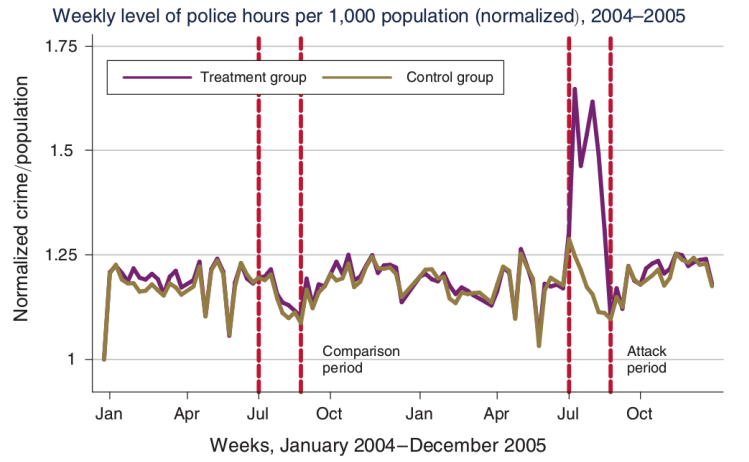
\includegraphics[width=7cm]{photos/2sls panel 1.png} }}%
    \qquad
    \subfloat[\centering Total Crimes (per 1,000 population)]{{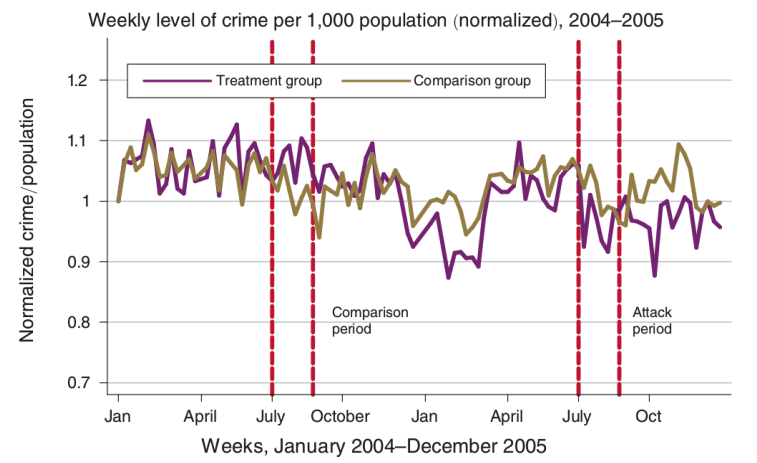
\includegraphics[width=7cm]{photos/2sls panel 2.png} }}%
    \caption{Figures from Draca et al.}%
    \label{fig:2sls panel example}%
\end{figure}

\begin{example}
    (cont.) Results from diff-in-diff:

    \begin{itemize}
        \item Police hours increased greatly in affected boroughs following the attacks
        \item no corresponding decline in control boroughs: increased hours from overtime
        \item relative to control periods there is less crime in the treatment boroughs
    \end{itemize}
    This does not really tell us how big the effect of police on crime is, i.e. elasticity. So, they created a 2SLS model.

    \begin{equation}
\text { crime }_{b t}=\delta \text { police }_{b t}+\boldsymbol{\lambda} \mathbf{X}_{b t}+\mu_b+\tau_t+\underbrace{\eta_{b t}+e_{b t}}_{\equiv \epsilon_{b t}}
\end{equation}
they have data from London boroughs, $b$, over time $t$.
\begin{itemize}
    \item $\boldsymbol{X}_{bt}$ is a vector of controls
    \item $\mu_b$ is a borough fixed effect
    \item $\tau_t$ is a common time effect
    \item $\eta_{bt}$ is a borough- and time-specific effect (e.g. exhibition drawing crowds)
\end{itemize}

First, they get rid of the borough fixed effects, $\mu_b$ by first differencing:
\begin{equation}
\Delta \text { crime }_{b t}=\delta \Delta \text { police }_{b t}+\boldsymbol{\lambda} \Delta \mathrm{X}_{b t}+\Delta \tau_t+\Delta \eta_{b t}+\Delta e_{b t}
\end{equation}
\begin{note}
    We could still have time-varying unobservables $\Delta \eta_{bt}$
\end{note}
They propose to use the terror attack as an instrument for the change in police hours $\Delta \text{police}_{bt}$. Technically it is $T_b \times POST_t$.

Our first stage is:
\begin{equation}
\Delta \text { police }_{b t}=\pi_1\left(T_b \times P O S T_t\right)+\boldsymbol{\pi}_2 \Delta X_{b t}+\Delta \psi_t+\Delta u_{b t}
\end{equation}

And our first-differenced model for crime is the \textbf{structural equation}
\begin{equation}
\Delta \text { crime }_{b t}=\delta \Delta \text { police }_{b t}+\boldsymbol{\lambda} \Delta \mathrm{X}_{b t}+\Delta \tau_t+\Delta \eta_{b t}+\Delta e_{b t}
\end{equation}
\begin{note}
    Notice the exclusion restriction
\end{note}

Results from 2SLS:

\begin{itemize}
    \item The substantial deployment of police had an immediate negative effect on crime
    \item As soon as police were withdrawn, crime went back up.
    \item This was all mostly driven by reductions in thefts and violence
\end{itemize}

The key in IVs is often whether the exclusion restriction holds. They argue at length why they think it does.
\end{example}

\subsection{Simultaneous Equation Models}

Another source of endogeneity is \textbf{simultaneity bias}. Explanatory variables might be jointly determined with the dependent variable. This could arise when e.g. an outcome is determined by a market equilibrium.

Let us consider trying to estimate the labour supply elasticity of workers. We have a simple labour supply function:
\begin{equation}
    \label{sem simple labour supply}
    h_s = \alpha_1 w + \beta_1 z_1 + u_1
\end{equation}

where $h_s$ is hours worked, $w$ is wage, $z_1$ is a variable affecting labour supply e.g. non-labour income, and $u_1$ is any other factors affecting labour supply (our error). \textbf{This is a structural equation}.

Suppose the demand for labour is given by:
\begin{equation}
    \label{sem simple labour demand}
    h_d = \alpha_2 w + \beta_2 z_2 + u_2
\end{equation}
$z_2$ can be thought of as a factor that shifts the demand for labour e.g. rainfall in the agricultural labour market. This is \textbf{also a structural equation}.

Consider a dataset at the country level, assume for country $i$:
\[h_{is} = h_{id}\]
\begin{note}
    we cannot distinguish $h_{is}$ and $h_{id}$. We just use $h_i$, observed hours.
\end{note}

Therefore we have the following equations:
\begin{equation}
\label{SEM 1}
    \begin{aligned}
        h_i &= \alpha_1 w + \beta_1 z_{i1} + u_{i1} \\
        h_i &= \alpha_2 w + \beta_2 z_{i2} + u_{i2}
    \end{aligned}
\end{equation}

This is a \textbf{simultaneous equations model (SEM)} jointly determining $h_i$ and $w_i$. Because $h_i$ and $w_i$ are determined within the model, they are \hl{endogenous variables}. $z_{i1},z_{i2}$ are determined outside of the model and therefore exogenous.
\begin{note}
    this is an assumption, it means that $z_{i1},z_{i2}$ re uncorrelated with $u_{i1}$ and $u_{12}$.
\end{note}

In SEMs the endogenous variables are correlated with the error term and therefore OLS estimates of $\alpha_1$ and $\alpha_2$ will be biased and inconsistent. 
\begin{note}
    This can be seen by rewriting wages as a function of exogenous variables only (assuming $\alpha_1 \neq \alpha_2$):
    \begin{equation}
w_i=\pi_{11} z_{i 1}+\pi_{12} z_{i 2}+\frac{1}{\alpha_2-\alpha_1}\left(u_{i 1}-u_{i 2}\right)
\end{equation}
where $\pi_{11} = \beta_1 / (\alpha_2 - \alpha_1)$, and $\pi_{12} = -\beta_2 / (\alpha_2 - \alpha_1)$.

Because $w_i$ is a function of $u_{i1}$ they will be correlated and therefore our OLS estimates of $\alpha_1$ suffer from simultaneity bias.
\end{note}

Now consider the SEM, but assume we only have data on hours, wage and rainfall:
\begin{equation}
\label{SEM 2 only rain}
\begin{aligned}
& h_i=\alpha_1 w_i+u_{i 1} \\
& h_i=\alpha_2 w_i+\beta_2 z_{i 2}+u_{i 2}
\end{aligned}
\end{equation}

If we are interested in estimating the labour supply elasticity we need exogenous variation in $w_i$ in the first equation. THis requires a demand shifter $z_{i2}$. 
\begin{example}
    $\uparrow z_{i2}$ could mean a lot of rainfall, which could mean more labour demanded by producers at the same wage (giving upward pressure on $h_i$, which would lead to a new market equilibrium at higher wages and higher labour supply.
\end{example}

This means that we would observe household labour supply react to increasing ages from an exogenous source, meaning $z_{i2}$ \textbf{traces out the labour supply curve}.

This logic suggests we can use $z_{i2}$ as an instrument for $w_i$ in the labour supply equation. This requires instrument relevance ($\beta_2 \neq0)$ and instrument exogeneity ($cov(z_{i2},u_{i1})=0$) (implies an exclusion restriction).

Under these assumptions, IV consistently estimates $\alpha_1$.

\clearpage
\section{Logit, Probit, Tobit}

There are many situations in which OLS is not suitable. These situations often arise from limited dependent variables.

\subsection{Limited Dependent Variables}

Limited dependent Variables consist of examples like:
\begin{itemize}
    \item Binary Variables
    \item Non-Negative Variables
    \item Non-Negative with Excess zeros
    \item Count Variables
    \item Censored Variables
\end{itemize}

It is easy to see situations in which these may arise e.g. wages (non-negative), employment (binary) etc.


\subsubsection{Binary Variables}

With our binary dependent variable $y=\{0,1\}$, we can create models. OLS is based on
\[E(y|x) = \beta_0 + \beta_1 x\]

With a binary dependent variable
\[E(y|x) = 0 \times P(y=0|x) + 1\times P(y=1|x) = P(y=1|x)\]

We call this the \textbf{linear probability model} (LPM):
\begin{equation}
    \label{linear probability model}
    P(y=1|x) = \beta_0 + \beta_1 x
\end{equation}
\begin{note}
    $\beta_1$ is now interpreted as the partial effect of $x$ on the probability of the observation $y=1$. Also, this model is problematic as it can result in probabilities greater (lower) than 1 (0).
\end{note}

\begin{shaded}
There are two potential problems with this:
\begin{enumerate}
    \item \textbf{Predictions}: It should hold that $0\leq \hat{P}(y=1|x) \leq1$. Then, the support of predictions is bounded between 0 and 1, but \hl{this does not hold since the LPM-based predictions have unbounded support.}

    \item \textbf{Heteroskedasticity}: By construction, there will be heteroskedasticity in our estimation.
    \begin{equation}
        \begin{aligned}
        u &= y-\beta_0 - \beta_1 x \\
        u =& \begin{cases}
            - \beta_0 - \beta_1 x & \text{ if } y = 0 \\
            1 - \beta_0 - \beta_1 x & \text{ if } y = 1
        \end{cases}
        \end{aligned}
    \end{equation}
    which implies
    \begin{equation}
        \label{heteroskedasticity in LPM}
        var(u|x) = (\beta_0 + \beta_1 x)(1 - \beta_0 - \beta_1 x)
    \end{equation}
    which is not constant.
\end{enumerate}
\end{shaded}

\begin{figure}[h]
    \centering
    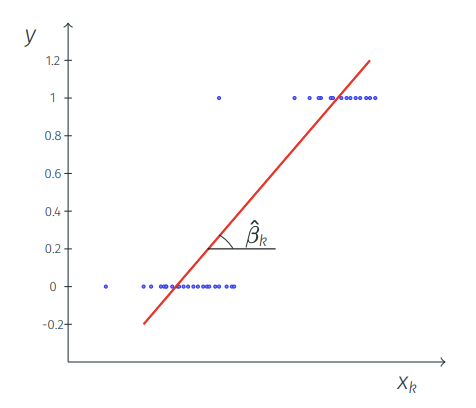
\includegraphics[width=10cm]{photos/LPM.png}
    \caption{Linear Probability Model}
    \label{fig:LPM}
\end{figure}

You can see clearly in Figure \ref{fig:LPM}, that if our $x$ value is below the lower intersection with the fitted values, we will get a probability, $\hat{y}$, that is lower than 0.


\subsection{The models}

To combat the limitations of the LPM, we can use non-linear models. Specifically in our case with the binary regressor, it is useful to have a non-linear model as our support is bounded.

Our non-linear models for binary response
\[P(y=1|x) = G(\underbrace{\beta_0 + \beta_1 x_1+ \ldots + \beta_k x_k}_{\text{Linear Index}}) = G(\boldsymbol{x\beta})\]

That linear index will return a single number, like normal, but then we use our $G(.)$ function to map this scalar onto the (0,1) interval. We look specifically at the Probit and Logit Models.

\begin{definition}
    \textbf{Probit}:
    \begin{equation}
        \label{Probit}
        G(z) = \Phi (z) = \int_{-\infty}^\infty \phi (v) dv
    \end{equation}
    where $\phi(v)$ is the probability distribution function (pdf).
\end{definition}

\begin{definition}
    \textbf{Logit Model}:
    \begin{equation}
        \label{logit}
        G(z) = \Lambda(z) = \dfrac{\exp(z)}{1+\exp{z}}
    \end{equation}
\end{definition}


\begin{figure}[h]
    \centering
    \subfloat[\centering Probit Cumulative Distribution Function]{{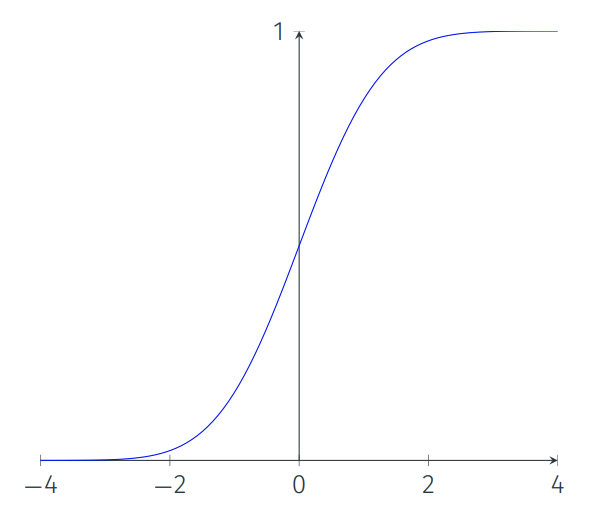
\includegraphics[width=7cm]{photos/probit dist.png} }}%
    \qquad
    \subfloat[\centering Logit Cumulative Distribution Function]{{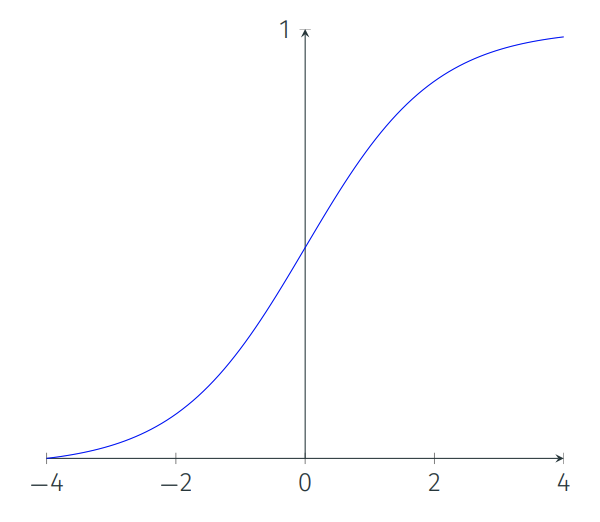
\includegraphics[width=7cm]{photos/logit dist.png} }}%
    \caption{The Probit and Logit CDFs}%
    \label{fig:probit logit cdf}%
\end{figure}


\begin{figure}[h]
    \centering
    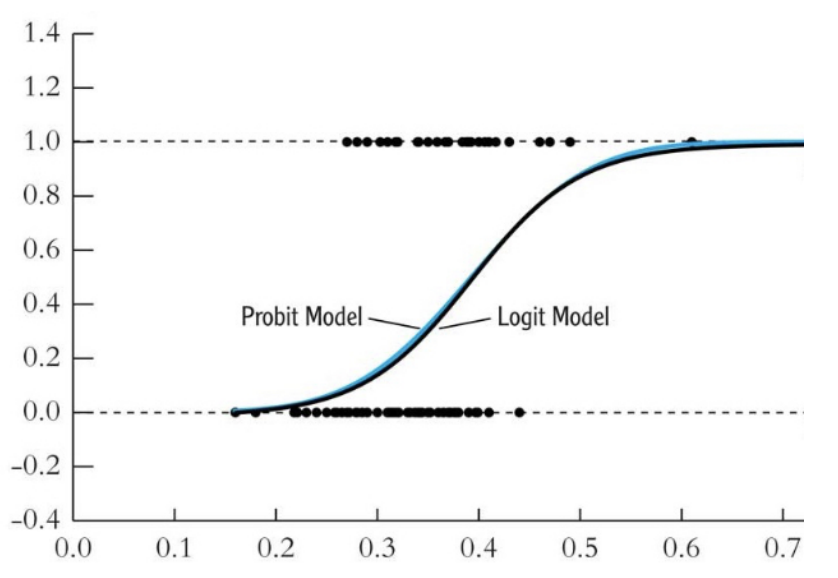
\includegraphics[width=9cm]{photos/logit vs probit.png}
    \caption{Comparing Probit and Logit}
    \label{fig: probit vs logit}
\end{figure}

\begin{note}
    In Figure \ref{fig: probit vs logit} in the middle section, both models are very similar to the linear model. Meaning, at the average, the linear probability model is very similar to the rest.
\end{note}


\begin{procedure}
    We use latent variable formulation to derive logit and probit. That is
    \[y^* = \boldsymbol{x\beta} + \epsilon, \quad x \indep \epsilon.\]

    $y^*$ is latent, i.e unobservable, so
    \[y \begin{cases}
        1 & \text{ if } y^*>0 \\
        0 & \text{ if } y^* \leq 0
    \end{cases}\]
    or equivalently
    \[y = 1[y^*>0]\]

    which gives us
    \begin{align*}
        P(y=1|\boldsymbol{x}) &= P(y^*>0|\boldsymbol{x}) \\
        &= P(\epsilon> - \boldsymbol{x\beta})
    \end{align*}

    
\end{procedure}

Logit and Probit then result from what we assume about the distribution of the error term
    \begin{itemize}
        \item If $\epsilon \sim N(0,1)$ 
        \[P(\epsilon > - \boldsymbol{x\beta}) = 1 - \Phi (-\boldsymbol{x\beta}) = \phi(\boldsymbol{x\beta})\]
        which explains why \textbf{probit} picks $G(\boldsymbol{x\beta}) = \Phi( \boldsymbol{x\beta})$
        \item If $\epsilon$ has the standard logistic distribution
        \[P(\epsilon > - \boldsymbol{x\beta}) = 1- \Lambda (- \boldsymbol{x\beta}) = \Lambda(\boldsymbol{x\beta})\]
        so \textbf{logit} picks $G(\boldsymbol{x\beta}) = \Lambda(\boldsymbol{x\beta}) = \frac{\exp{(\boldsymbol{x\beta})}}{1 + \exp{(\boldsymbol{x\beta})}}$
    \end{itemize}


\subsection{Estimation}

We use Maximum Likelihood Estimation (MLE) for Probit and Logit models. That is, we find estimators that maximise the probability of observing the sample we have.

\subsubsection{Probit Example}

If we are using Probit, we know
\[P(y=1|x) = \Phi(\beta_0 + \beta_1 x)\]

Given our sample:
\begin{table}[h]
    \centering
    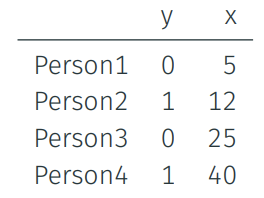
\includegraphics[width=7cm]{photos/probit example sample.png}
    \caption{Example Sample}
    \label{tab: probit example sample}
\end{table}

What is the probability of observing this sample? If we calculate person by person:
\begin{align*}
    \text{Person 1: } & P(y=0|x=5) = 1-P(y=1|x=5) = 1-\Phi(\beta_0 + \beta_1 \times5) \\
    \text{Person 2: } & P(y=1|x=12) = \Phi(\beta_0 + \beta_1 \times12) \\
    &\vdots
\end{align*}

The joint probability of observing this sample \textit{under random sampling}:
\[p(y=0|x=5) \times P(y=1|x=12) \times P(y=0|x=25) \times P(y=1|x=40)\]

Writing this more compactly in terms of the conditional density, the \textbf{likelihood contribution} of observation $i$ is:
\[f(y_i|\boldsymbol{x}_i;\boldsymbol{\beta}) = [G(\boldsymbol{x_i\beta})]^{y_i}[1-G(\boldsymbol{x_i\beta})]^{1-y_i}.\]

The \textbf{likelihood function} of the sample is:
\[L(\boldsymbol{\beta}) = f(y_1|\boldsymbol{x}_1;\boldsymbol{\beta}) \times f(y_2|\boldsymbol{x}_2;\boldsymbol{\beta}) \times \ldots \times f(y_n|\boldsymbol{x}_n;\boldsymbol{\beta})\]

By taking logs we get the log-likelihood function:

\begin{equation}
    \label{log likelihood function - probit example}
    \mathcal{L}(\boldsymbol{\beta}) = \sum_{i=1}^n y_i \log [G(\boldsymbol{x_i\beta})] + (1-y_i)\log [1-G(\boldsymbol{x_i\beta})]
\end{equation}
where $\hat{\boldsymbol{\beta}}$ is the value of $\boldsymbol{\beta}$ that maximises this function and is called the \hl{maximum likelihood estimator}.

\begin{shaded}
\subsubsection{MLE Properties}
\begin{itemize}
    \item Under standard assumptions the MLE is consistent and asymptotically normal/efficient.
\end{itemize}

The most important assumptions are:
\begin{enumerate}
    \item The model is \textbf{correctly specified}
    \item We have a \textbf{random sample}
    \item $\epsilon \indep x$
    \item There is \textbf{no perfect collinearity}
\end{enumerate}

Inference is based on \textbf{asymptotic errors}. We are unable to do t-tests because we do not have a finite sample.
\end{shaded}

\subsection{Inference}

Using the example from lectures, we are finding what the effect of class and gender had on the survival rate in the Titanic.

\begin{figure}
    \centering
    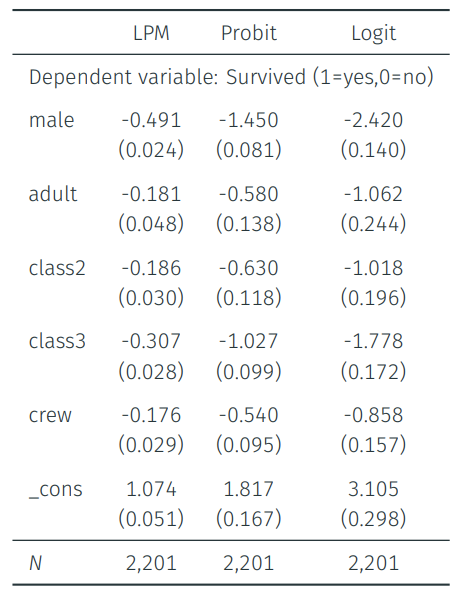
\includegraphics{photos/titanic results.png}
    \caption{Results from Titanic regression, using different estimation techniques}
    \label{fig: titanic inference}
\end{figure}

\begin{note}
    The Probit and Logit coefficients are meaningless without transformation, they are showing the effects on a latent variable $y^*$.
\end{note}

So, say we are interested in the probability that a young girl in first class survived the Titanic, then we can do this:

\begin{align}
    &\boldsymbol{\hat{P}(y=1| \text{girl in first class})} \\
    \text{LPM:} & \quad \beta_0 = 1.074 \\
    \text{Probit:} & \quad \Phi(\beta_0) = \Phi(1.817) = 0.965 \\
    \text{Logit:} & \quad \Lambda(\beta_0) = \Lambda(3.105) = 0.957
\end{align}

If we wanted to compare the probability of a young girl and a grown woman in first class we can see:

\begin{align}
    \text{LPM:} & \quad \Delta P = \beta_{2} = -0.181 \\
    \text{Probit:} & \quad \Delta P = \Phi(\beta_0 + \beta_{adult}) - \Phi(\beta_0) = \Phi(1.817-0.58) - \Phi(1.817)  = - 0.073\\
    \text{Logit:} & \quad \Lambda(\beta_0 + \beta_{2}) - \Lambda(\beta_0) = \Lambda(3.105 - 1.062) - \Lambda(3.105)  = - 0.07
\end{align}

\begin{note}
    The probit/logit estimation does not hold everything constant, that is, each person/group has its own effect. The difference between a young girl and a grown woman surviving will not be the same as the difference between a young boy and a grown man surviving, for example.
\end{note}

\subsection{Partial Effects}

Our model for the probability of survival is
\begin{equation}
P(y=1 \mid \boldsymbol{x})=G\left(\beta_0+\beta_1 \text { male }+\beta_2 \text { adult }+\beta_3 \text { class } 2+\beta_4 \text { class } 3+\beta_5 \text { crew }\right)
\end{equation}

The partial effect of an indicator variable (male), all other variables constant is
\begin{equation}
\begin{gathered}
\quad G\left(\beta_0+\beta_1 \text{ male }+\beta_2 \text { adult }+\beta_3 \text { class } 2+\beta_4 \text { class } 3+\beta_5 \text { crew }\right) \\
-G\left(\beta_0+\beta_2 \text { adult }+\beta_3 \text { class } 2+\beta_4 \text { class } 3+\beta_5 \text { crew }\right)
\end{gathered}
\end{equation}

\begin{procedure}
    Finding the partial effects in the LPM is simple.
    \begin{align*}
        P(y=1|x) =& \beta_0 \beta_1 x \\
        \dfrac{\partial P(y=1|x)}{\partial x} &= \beta_1
    \end{align*}

    This is much more confusing in the probit/logit cases.
    
    Probit:
    \begin{align*}
        P(y=1|x) &= \Phi(\beta_0 + \beta_1 x) \\
        \dfrac{\partial P(y=1|x)}{\partial x} &= \Phi^\prime (\beta_0 + \beta_1 x)\beta_1 = \phi(\beta_0 + \beta_1 x)\beta_1 
    \end{align*}

    The Logit is equivalent but with the logistic cumulative distribution function and probability distribution function.
\end{procedure}

\subsubsection{Interpretation of Coefficients}

\paragraph{Discrete Variables}\mbox{}

\[G(\beta_0 + \beta_1 x_1 + \ldots + \beta_k (c_k + 1) + \ldots + \beta_K x_K) - G(\beta_0 + \beta_1 x_1 + \ldots + \beta_k c_k + \ldots + \beta_K x_K)\]

\paragraph{Continuous Variables} \mbox{}

\[\dfrac{\partial P(y=1|x)}{\partial x_j} = g(\boldsymbol{x\beta})\beta_j\]

where $g(z) = \frac{\partial G(z)}{\partial z} >0$

\subsubsection{Additional Measure (APE, PEA)}

We have our partial effects of the explanatory variables
\[\dfrac{\partial P(y=1|x)}{\partial x_j} = g(\boldsymbol{x\beta})\beta_j.\]

The \textbf{partial effect at the average}:
\[\widehat{PEA}_j = g(\boldsymbol{\bar{x}\hat{\beta}})\hat{\beta}_j\]
In this, we are saying measuring the partial effect for the average person, is difficult to quantify and is problematic.

The \textbf{Average Partial Effect}:
\[\widehat{APE}_j = \dfrac{1}{n}\sum_{i=1}^N g(\boldsymbol{x_i\hat{\beta}})\hat{\beta_j}\]

\begin{table}[h]
    \centering
    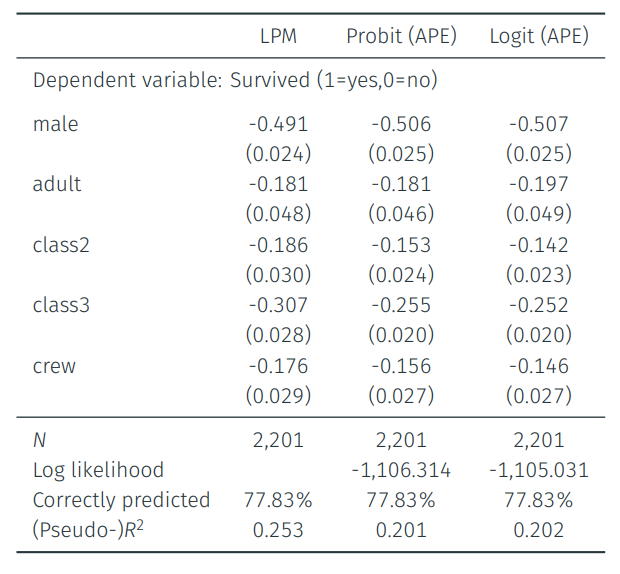
\includegraphics[width=10cm]{photos/APE example.png}
    \caption{LPM compared to the Average Partial Effect of Probit/Logit}
    \label{tab:APE results}
\end{table}

You can see from table \ref{tab:APE results}, that the APE of probit and Logit is extremely similar to the LPM. This is why in practice lots of people still use LPM, even though we know these flaws.

\begin{note}
    We cannot compare the logit and probit log-likelihoods. Additionally, because the OLS $R^2$ does not work for probit/logit, we use a pseudo-$R^2$.
\end{note}

\subsection{Testing}
\subsubsection{Goodness-of-fit}
The goodness-of-fit (GOF) measures for Probit/Logit:
\begin{mdframed}

\paragraph{Percent correctly predicted}\mbox{}

\[\text{ correct if} \begin{cases}
    y_i = 1 &\text{ and  } G(\boldsymbol{x_i \hat{\beta}) \geq \tau} \\
    y_i = 0 &\text{ and } G(\boldsymbol{x_i \hat{\beta}}) < \tau
\end{cases}\]

That $\tau$ is arbitrary, e.g. $\tau = 0.5, \tau = \bar{y}$. Our percent correctly predicted measure can be used on LPM too.
\end{mdframed}

\begin{mdframed}
\paragraph{Pseudo-R Squared} \mbox{}
Because we cannot use our normal $R^2$, we use a pseudo-$R^2$. The equation for this is:
\begin{equation}
    \label{pseudo r squared}
    \Bar{R}^2 = 1 - \dfrac{\mathcal{L}_{ur}}{\mathcal{L}_0}
\end{equation}
where $\mathcal{L}_{ur}$ is the log-likelihood of the \textbf{estimated (unrestricted) model}, and $\mathcal{L}_0$ is the log-likelihood of the model with \textbf{only the intercept}
\end{mdframed}

\begin{mdframed}
    \paragraph{Correlation based measures} \mbox{}
    \[corr(y_i, G(\boldsymbol{x\beta}))\]
\end{mdframed}

\subsubsection{Hypothesis Testing}

Our usual tests and confidence intervals can be used, but they are based on asymptotic approximations. That is
\[\boldsymbol{\hat{\beta}} \overset{app}{\sim} N(\boldsymbol{\beta}, var(\boldsymbol{\hat{\beta}}))\]

therefore, if we want to test $H_0: \beta_1 = 0, H_1: \beta_1 \neq 0$, we can
\[z = \dfrac{\hat{\beta}_1}{se(\hat{\beta}_1)}\]

Just as before $p = 2[1-\Phi(|z|)]$ and we reject $H_0$ if $|z|>z_{crit}$. 1.96 at 5\% level. This is a simple \hl{Wald test}.

\paragraph{Wald Test}\mbox{}

The Wald test can be extended to test $q$ restrictions (like an F test). The Wald statistic has an asymptotic $\chi_q^2$ distribution. \textbf{It is calculated with estimation under only the alternative hypothesis}, the unrestricted model.

\paragraph{Likelihood Ratio test} \mbox{}

We \textbf{must estimate two models}, one restricted, one unrestricted. Example:
\[\boldsymbol{\hat{\beta}_{ur}}= \left[\hat{\beta}_0 \quad \hat{\beta}_1 \quad \hat{\beta}_2\right]\]
and 
\[\boldsymbol{\hat{\beta}_r} = \left[\hat{\beta}_0\right]\]

Clearly $\mathcal{L}(\boldsymbol{\hat{\beta}_{ur}}) \geq \mathcal{L}(\boldsymbol{\hat{\beta}_{r}})$. A large drop in log-likelihood indicates that the excluded variables are important to explain the data.

The \textbf{Likelihood Ratio statistic}:
\[LR = 2\left[\mathcal{L}(\boldsymbol{\hat{\beta}_{ur}}) - \mathcal{L}(\boldsymbol{\hat{\beta}_{r}}) \right]\]

if we are testing $q$ restrictions
\[LR \overset{app}{\sim}\chi_q^2\]

\paragraph{Example: Titanic} \mbox{}

\begin{figure}[h]
    \centering
    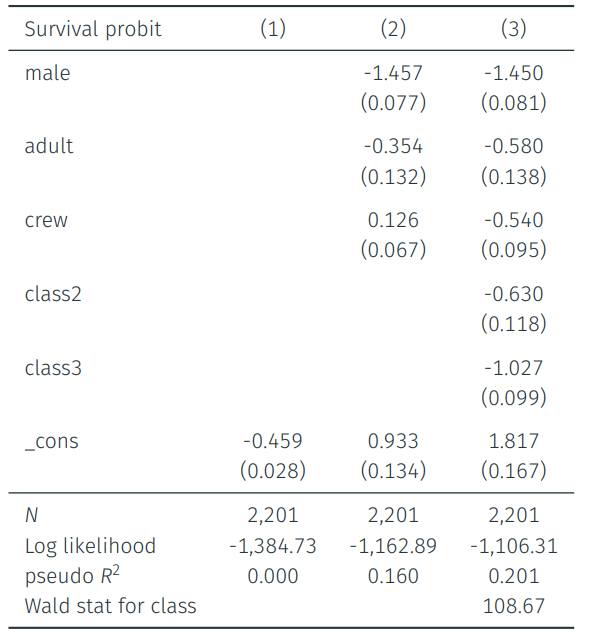
\includegraphics[width=12cm]{photos/LR example probot.png}
    \caption{Different Probit Models}
    \label{fig: LR example}
\end{figure}

Testing Model (1) compared to Model (2):
\begin{align*}
    LR &= 2[-1162 - (-1384.73)]\\
    & = 443.68
\end{align*}

This is obviously greater than our critical value of 7.81. In this test, we are testing \textbf{3 restrictions}.

\subsection{Tobit}

We have looked at the case where our dependent variable is binary, but we have other limitations to the dependent variable as we discussed earlier. Another case is non-negative dependent variables. In this case, we use \textbf{Tobit} estimation.












\end{document}